\documentclass{src/dutmsc}%
%\documentclass[draft]{src/dutmsc}%
%
% STARTING FROM VERSION 1.0.8, DIRECT PDF OUTPUT FROM THE LATEX SOURCE IS SUPPORTED.
% IF YOU WANT TO USE THIS FEATURE, MAKE SURE ALL YOUR OWN FIGURES ARE IN A FORMAT
% SUPPORTED BY PDFLATEX, SO no EPS FILES, BUT PDF OR JPEG OR SO.
% THIS HAS CONSEQUENCES FOR THE PACKAGES USED AS WELL, pstricks CANNOT BE USED WITH PDFLATEX
%
% fill the following with relevant information
\mscDepartment{Aerodynamics and Wind Energy}%
\mscFaculty{Aerospace Engineering}%
\mscName{L. Manickathan B.Sc.}%
\mscDate{Date TBD}%
\mscTitle{Hybrid Vortex Method for 2D Vertical-Axis Wind Turbine}%
\mscSubTitle{A fast and accurate Eulerian-Lagrangian numerical method in python}% can be left empty
\mscKeyWords{Hybrid Vortex Method, Python}%
%
% background picture for the first page, make sure it is in the correct format (eps or something else)
%%\ifpdfma
%  \mscBackPicture{./figs/merlin_landing_3_pdf}    % eps of 21 * 29.7 cm
%\else
%  \mscBackPicture{./figs/merlin_landing_3}    % pdf version of the cover background
%\fi
%
% readers page (un)comment as necessary
\mscReaderOne{prof.dr.ir. G.J.W. van Bussel}
\mscReaderTwo{dr.ir. C.J. Simao Ferreira}
\mscReaderThree{dr.ir. A. Palha da Silva Clerigo}
\mscReaderFour{prof.dr.ir. I. Bennett}
% \mscReaderFive{ir. Reader Five}
% \mscReaderSix{ir. Reader Six}
%
% if defined here with a non-zero (e.g. 1) argument, an entry will be added to 
% the table of contents for the list of figures and the list of tables,
% else they will not appear in the toc.
\loflotintoc{1}
%
% default install of latex on linux (tetex) does not include the apacite package, so using a local version
% if your latex distribution does provide it, you can uncomment the next two lines (and comment
% the two lines after that)
% \usepackage{apacite}%
% \bibliographystyle{apacite}%
% \usepackage{./local/apacite/apacite}%
%
% If you prefer references as numbers, comment the following line and uncomment the one thereafter
% \bibliographystyle{./local/apacite/apacite}%
\bibliographystyle{plain}
%
%
% use package breakurl to break url in sensible places (such as in www references)
% if it is not available in your latex distribution, use the local one
%\usepackage[preserveurlmacro]{./local/breakurl/breakurl}
\usepackage[preserveurlmacro]{breakurl}% %% Uncommented due to warning
%\usepackage{./local/breakurl/breakurl}%
%\usepackage{breakurl}% 
%
%=================%
% custom commands %
%=================%
%
% short-hand notations for cosine, sine and tangent with calligraphic C, S and T
\newcommand{\cc}[1]{\:\mathcal{C}_{#1}}%
\newcommand{\cs}[1]{\:\mathcal{S}_{#1}}%
\newcommand{\ct}[1]{\:\mathcal{T}_{#1}}%
%
% matlab in small caps
\newcommand{\matlab}{\textsc{Matlab} }
\newcommand{\python}{\textsc{Python} }
%
%\newcommand{\printAbbreviation}[3]{#1 (\textcolor{darkblue}{#2}) \nomenclature[#3]{#2}{#1}}

\makenomenclature
%
% setup of hyperlinks in the pdf output (modify as needed)
\hypersetup{colorlinks=true,
            citecolor=darkblue,
            urlcolor=darkred,
            linkcolor=darkblue,
            menucolor=darkblue,
            anchorcolor=red,
            pagecolor=cyan,
            pdfborder={0 0 0},
            bookmarksnumbered=true,
            breaklinks=true,
            pdfauthor={\mscname},           % value of \mscName
            pdftitle={\msctitle},           % value of \mscTitle
            pdfkeywords={\msckeywords}}     % value of \mscKeywords
%
\renewcommand{\bibname}{References}

\usepackage{amsmath}
\usepackage{amsfonts}
\usepackage{amssymb}
\usepackage{graphicx}
\usepackage{hyperref}
\usepackage{python}

\usepackage{graphicx}
\usepackage{caption}
\usepackage{color}


\newcommand{\printAcron}[2]{#1 ({\color{darkblue}{#2}}) \acron[f]{#2}{#1}}
\begin{document}%


%============================= Front matter ========================================
\frontmatter%
    %
    \maketitle%
    %
    % Abstract/summary
    \nonumchap{Summary}
    %
    This is the summary of the thesis.
%
    \cleardoublepage%
    %
    % thank people in this file
    \nonumchap{Acknowledgements}
    %
    
    The work I present here would not have been possible without the support of my supervisors dr.ir. C. (Carlos) J. Simao Ferreira and dr.ir. A. (Artur) Palha da Silva Clerigo. I want to thank Carlos for the constant encouragement and ensuring that I didn't loose myself in the detail and to have a global picture. Thank you for also giving me fresh perspective when it seems impossible and making me to think outside the box. I want to thank Artur for his daily supervision and guidance to teach me all the intricate details for developing this numerical method. I also want to thank him for putting aside time to work hand-in-hand to find solutions to the problems I faced and supporting me throughout the thesis.
    
    I want to thank my friends: Chid, Thor, Oliver, Mark, Rob, Alberto, Hector, Rody and Dieter for spending time together at the university, tackling the challenge of finishing the master thesis together. You guys gave me joy during the work and it was fun working beside you guys. I want to thank my friends: Nik, Vis, Adi, Srij, Ash, Vipul, Abi, Ram, Darsini, Yu, Ken, Gary, Hemmo and Dennis for making my last few years in Netherlands an enjoyable experience.
    
    Finally, I want to thank my family: Daddy, Mummy, Chechi, and Denis Chettan. Thank you for your patience and your unending love throughout my life.
    
    % signature containing place, name and date
    \signature
%
    \cleardoublepage%
    % 
    % table of contents, list of figures and list of tables
    \tocloflot%
    %
    % Nomenclature
    \printnomencl%      
    \cleardoublepage%
        
    %
    %
\mainmatter%
    %
    % parts are not necessary for a thesis
    %
    % Example Chapter
    %\chapter{Introduction}
    %
    \section{Before You Start}
        %
        RTFM\footnote{Read The Fabulous Manual ;-)}: \href{http://www.ctan.org/tex-archive/info/lshort/english/lshort.pdf}{The Not So Short Introduction to \LaTeXe}.
        %
        Chapters 1, 2 and 3 are a must.
        
        And you directly see why \LaTeX~is so much easier than Word, external references actually work.
        %
        %
    \section{Quick Compilation of Your Thesis}
        %
        To quickly compile your thesis without processing all figures, add \verb+draft+ to the list of optional arguments of the main file (\verb+my_thesis.tex+ in this case):
        %
        \begin{verbatim}
    \documentclass[draft]{dutmsc}%
        \end{verbatim}
        %
        The actual figures will not appear, only a border will be shown. This reduces the compilation time by a significant amount. The command \verb+\includeonly{filelist}+ can also be used to only process the chapter you are working on at the time.
        %
    \section{Custom Commands}
        %
        \subsection{Vertical Spacing in Tables}
            %
            Look at Table~\ref{tab:sample_table}. Iz nice, no?
            %
            \begin{table}[!htb]
                \centering
                \begin{tabular}{ c c c }
                    \hline
                    Param\T\B                   & Value   & Unit    \\
                    \hline
                    $v_i$\T                     & 11.47   & $[m/s]$ \\
                    $\Omega R$                  & 212.25  & $[m/s]$ \\
                    $\lambda_i$\B               & 0.054   & $[-]$   \\
                    \hline
                \end{tabular}
                \caption{Improved vertical spacing in tables}\label{tab:sample_table}
            \end{table}
            %
            It uses two custom commands to add some space just after (bottom) and before (top) a horizontal line, \verb+\B+ and \verb+\T+. Without them, the table would look really bad (see Table~\ref{tab:sample_table2}).
            
            %
            \begin{table}[!htb]
                \centering
                \begin{tabular}{ c c c }
                    \hline
                    Param                       & Value   & Unit    \\
                    \hline
                    $v_i$                       & 11.47   & $[m/s]$ \\
                    $\Omega R$                  & 212.25  & $[m/s]$ \\
                    $\lambda_i$                 & 0.054   & $[-]$   \\
                    \hline
                \end{tabular}
                \caption{Default vertical spacing in tables}\label{tab:sample_table2}
            \end{table}
            %
        \subsection{Shorthand Notations for Sine, Cosine and Tangent}
            %
            Three commands are available to display sine, cosine and tangent of angles in math mode: $\cc{\alpha}$, $\cs{\beta}$, $\ct{\gamma}$.
            %
        %
    \section{Bibliography/References}%
        %
        These are some references just for the sake of it. If you want to know more about ground effect models, consult~\cite{xin_phd}.
        For an introduction into helicopter aerodynamics, read~\cite{leishman_book}. And a reference to LAPACK~\cite{lug}.
        If you need to know more about the display options for citations, read the documentation that is provided in its manual \url{./local/apacite/apacite.pdf}.
        
        This thesis uses a bib-file (named \verb+biblio.bib+), which contains a database of references. \LaTeX~collects those references that were referred to in the thesis, and store them in the \verb+*.aux+ files (for this chapter in \verb+chap_introduction.aux+). And as long a the program \verb+bibtex+ is not executed, \LaTeX~will complain about undefined citations and a missing \verb+.bbl+ file (in this case \verb+my_thesis.bbl+). To solve this, execute \verb+bibtex+. If everything goes as it should, a \verb+my_thesis.bbl+ is created, and the next time you run \LaTeX, a section with references will appear.
        
        Using \verb+Kile+ (on Linux), BibTex can be executed from the \verb+Build -> Compile -> Bibtex+ menu, or using the shortcut \verb/ALT+-/ (as in ALT+minus).
        
        Using \verb+TeXnicCenter+, BibTex can be executed from the \verb+Build -> BibTex+ or \\
        \verb+Build -> Current File -> BibTex+ menu.
        
        Using \verb+WinEdt+, BibTex can be executed with the shortcut \verb/CTL+SHIFT+B/ or from the menu \verb/Accessories -> BibTex/.
        %
    \section{Symbols and Units}%
        %
        For symbols, we use the \verb+nomencl+ package, of which you need the latest version (version 4.2, dated 2005/09/22).
        %
        \subsection{Summary of Commands}
            %
            For nomenclature (symbols and abbreviations) to appear in the nomenclature chapter, the following 6 categories are available:
            
            \begin{description}
                \item[Latin Symbols]    \verb+\lsymb[t]{symbol}{description}{unit}{sortsymbol}+
                \item[Greek Symbols]    \verb+\gsymb[t]{symbol}{description}{unit}{sortsymbol}+
                \item[Other Symbols]    \verb+\osymb[f]{symbol}{description}{sortsymbol}+
                \item[Superscripts]     \verb+\subscr[f]{symbol}{description}+
                \item[Subscripts]       \verb+\superscr[f]{symbol}{description}+
                \item[Abbreviations]    \verb+\acron[f]{abbreviation}{description}+
            \end{description}
            %
            The first option (with the square brackets) is an optional argument that lets you control the appearance of the symbol in the text at the place where the command appears. If it is equal to \emph{t}, the symbol will appear in the text and in the nomenclature list and otherwise, it will only appear in the nomenclature list. By default, Greek and Latin symbols will appear in the text, even if the optional symbol is not set. In case they should not appear, you have to add \verb|[f]| as first argument. In the above list, the default values are given, so by default, only the Greek and Latin symbols will appear in the text at the place where the commands appear.
            
            Now, if you want these symbols to appear in the \emph{Nomenclature list}, execute \verb+makeindex+\footnote{Note that makeindex is a program on your computer. It is not a \LaTeX~command!}:
            %
            \begin{small}
            \begin{verbatim}
   makeindex $THESIS_NAME.nlo -s nomencl.ist -o $THESIS_NAME.nls
            \end{verbatim}
            \end{small}
            %
            where \verb+$THESIS_NAME+ is the name of the main file (without extension), in this case \verb+my_thesis+. Depending on the editor you use, it may not be necessary to resort to command line magic, you might just have to press a button that defines a macro. Another solutions is to use the \emph{bat} file included in the same directory: \verb+sort_symb.bat+. Executing this should do the above automagically.
            
            %
            \subsubsection{Sorting Symbols}
                %
                To sort symbols properly, an additional fourth mandatory argument is added to the Greek, Latin and Other symbols. These add the ability to sort similar symbols (such as \lsymb[t]{$\dot{m}$}{mass flow}{$[kg/s]$}{mz} and \lsymb[t]{$m$}{mass}{$[kg]$}{mm}) in the proper order ($m$ before $\dot{m}$). The way to make sure that the symbol for mass flow appears after the symbol for mass is shown below:%
                %
                \begin{small}%
                \begin{verbatim}
    \lsymb[t]{$m$}{mass}{$[kg]$}{mm}
    \lsymb[t]{$\dot{m}$}{mass flow}{$[kg/s]$}{mz}
                \end{verbatim}%
                \end{small}%
                %
                \verb+mz+ comes after \verb+mm+ when sorted by \verb+makeindex+, which means that the symbol of mass flow will be put after the symbol for mass.
                
                Something similar can be done for the Greek symbols. If \gsymb[t]{$\gamma$}{flight path angle}{$[rad]$}{3} (third letter in the Greek alphabet) should appear before \gsymb[t]{$\delta$}{some coefficient to show proper sorting of symbols}{$[-]$}{4} (fourth letter), add a letter to force proper sorting:
                %
                \begin{small}%
                \begin{verbatim}
    \gsymb[t]{$\gamma$}{flight path angle}{$[rad]$}{cc}
    \gsymb[t]{$\delta$}{some coefficient to show proper sorting of symbols}{$[-]$}{4}
                \end{verbatim}%
                \end{small}%
                %
                In table~\ref{tab:greek_symbols}, you can find the sort symbols (index) that I used to make sure that the Greek symbols appear in the correct order in the nomenclature.
                %
                \begin{table}[!ht]
                    \centering
                    \begin{tabular}{c c c | c c c}
                        \hline
                        Greek Symbol\T\B  & Command     & Index & Greek Symbol\T\B  & Command     & Index \\
                        \hline
                        $\alpha$\T  & \verb+\alpha+     & aa    & $o$         & \verb+o+          & oo    \\
                        $\beta$     & \verb+\beta+      & bb    & $\Pi$       & \verb+\Pi+        & p     \\
                        $\Gamma$    & \verb+\Gamma+     & c     & $\pi$       & \verb+\pi+        & pp    \\
                        $\gamma$    & \verb+\gamma+     & cc    & $\rho$      & \verb+\rho+       & qq    \\
                        $\Delta$    & \verb+\Delta+     & d     & $\Sigma$    & \verb+\Sigma+     & r     \\
                        $\delta$    & \verb+\delta+     & dd    & $\sigma$    & \verb+\sigma+     & rr    \\
                        $\epsilon$  & \verb+\epsilon+   & ee    & $\tau$      & \verb+\tau+       & ss    \\
                        $\zeta$     & \verb+\zeta+      & ff    & $\Upsilon$  & \verb+\Upsilon+   & t     \\
                        $\eta$      & \verb+\eta+       & gg    & $\upsilon$  & \verb+\upsilon+   & tt    \\
                        $\Theta$    & \verb+\Theta+     & h     & $\Phi$      & \verb+\Phi+       & u     \\
                        $\theta$    & \verb+\theta+     & hh    & $\phi$      & \verb+\phi+       & uu    \\
                        $\iota$     & \verb+\iota+      & ii    & $\chi$      & \verb+\chi+       & vv    \\
                        $\kappa$    & \verb+\kappa+     & jj    & $\Psi$      & \verb+\Psi+       & w     \\
                        $\Lambda$   & \verb+\Lambda+    & k     & $\psi$      & \verb+\psi+       & ww    \\
                        $\lambda$   & \verb+\lambda+    & kk    & $\omega$    & \verb+\omega+     & xx    \\
                        $\mu$       & \verb+\mu+        & ll    & $\Omega$\B  & \verb+\Omega+     & x     \\
                        $\nu$       & \verb+\nu+        & mm    &  &  & \\
                        $\Xi$       & \verb+\Xi+        & n     &  &  & \\
                        $\xi$       & \verb+\xi+        & nn    &  &  & \\
                        \hline
                    \end{tabular}
                    \caption{Sort symbols used to sort all Greek letters}\label{tab:greek_symbols}
                \end{table}
                %
        \subsection{More Examples}
            %
            The angle of attack \gsymb[f]{$\alpha$}{This is a very long explanation, and without this, it is still too short to show you what I want to show\ldots}{$[rad]$}{aa} (\verb+\gsymb[f]{\alpha}{Angle of attack}{$[rad]$}{aa}+) can be calculated from the pitch angle \gsymb{$\theta$}{Angle of pitch}{$[rad]$}{hh} (\verb+\gsymb{\theta}{Angle of pitch}{$[rad]$}{hh}+) and the flight path angle \gsymb{$\phi$}{Flight path angle}{$[rad]$}{uu} (\verb+\gsymb{\phi}{Flight path angle}{$[rad]$}{uu}+) as follows:
            %
            \begin{equation}
                \alpha = \theta + \phi\footnote{Note that the sign depends on the definition of the angles.}
            \end{equation}
            %
            Same thing for Latin symbols:
            
            \lsymb[t]{$\bar{x}$}{State vector of a dynamical system}{$[-]$}{xb}, for which the code looks like this:
            %
    \begin{verbatim}
    \lsymb[t]{$\bar{x}$}{State vector of a dynamical system}{$[-]$}{xb}
    \end{verbatim}
            %
            
            \begin{equation}\label{eq:state_vector_squared}
                \bar{x}^2 = \theta_i
            \end{equation}
            %
            \superscr[f]{2}{Square me}\subscr{i}{An index, or something\ldots}
            For subscripts and superscripts (as depicted in Eq~\ref{eq:state_vector_squared}), something special is needed. The sub- and superscripts must be added separately, as in:
            %
            \begin{verbatim}
    \superscr[f]{2}{Square me}\subscr{i}{An index, or something\ldots}
            \end{verbatim}
            %
            The commands for sub- and superscripts also have only two obligatory arguments, instead of three as is the case with the Latin and Greek symbols.
            
            Acronyms are also part of the nomenclature list. They are defined as follows:
            %
            \begin{verbatim}
    \acron[t]{PID}{Proportional -- Integral -- Derivative}
            \end{verbatim}
            %
            \acron[t]{P}{Proportional (Controller)}, 
            \acron[t]{PD}{Proportional -- Derivative (Controller)} and
            \acron[t]{PID}{Proportional -- Integral -- Derivative (Controller)} controllers.
            
            At last, there is a possibility for other symbols that do not fit in any of the above categories, such as symbols to denote matrices or vector quantities, such as \osymb[t]{$[\;]$}{matrix}, \osymb[t]{$\{\;\}$}{column vector} and \osymb[t]{$\bar{\;}$}{vector quantity}.
            %
    \section{Figures}
        %
        Up to version 1.0.7 of the style file, the only option to generate pdf output was throught the three-step process LATEX $\rightarrow$ DVI, DVI $\rightarrow$ PS, PS $\rightarrow$ PDF.
        
        Starting from version 1.0.8, direct pdf output is supported as well. This has some consequences for the file formats of figuress that are supported. When creating the pdf directly, figures in (encapsulated) postscript format will give errors. Convert them to pdf format.
        
        In all previous versions of this document, the advice in this section was to save all plots and figures as PostScript, and not as PDF. Processing your \LaTeX~input using LATEX $\rightarrow$ DVI, DVI $\rightarrow$ PS, PS $\rightarrow$ PDF works without problems. An added benefit is that you can use the \emph{psfrag} package to replace ordinary text characters in the postscript figures by e.g. mathematical formulas typeset in \LaTeX. Also, one can use the \emph{pstricks} packages to create figures (see~\href{http://www.tug.org/PSTricks/main.cgi/}{PSTricks packages}) directly in \LaTeX.
        
        The same can be achieved with plot output from e.g. {\sc matlab} using \emph{LaPrint}.
        
        LaPrint is a {\sc matlab} function to print {\sc matlab} graphics for inclusion in \LaTeX~documents. LaPrint creates an eps-file and a tex-file. The tex-file contains the annotation of the figure such as titles, labels and texts. The eps-file contains the non-text part of the figure and is called by the tex-file. 
        
        The main advantage of using LaPrint is that the annotation can be neatly (e.g., including math mode and fancy font constructs) set within \LaTeX. LaPrint can be used from the command line or via a graphical user interface (GUI).
        
        A Users Guide for LaPrint is available at \href{http://www.uni-kassel.de/fb16/rat/matlab/laprint/laprintdoc.ps}{\burl{http://www.uni-kassel.de/fb16/rat/matlab/laprint/laprintdoc.ps}}.
        The m-file can be downloaded from \href{http://www.mathworks.de/matlabcentral/fileexchange/4638}{Matlab File Exchange}.
        

        
%         {\LARGE For the best results and the least amount of headaches, save all your plots and figures as {\Huge PostScript}, not as PDF.}
%         
%         And process your \LaTeX~input using: LATEX $\rightarrow$ DVI, DVI $\rightarrow$ PS, PS $\rightarrow$ PDF. That way, you can use the \emph{psfrag} package to replace characters in a postscript file with formulas in the correct font, as will be shown below. Figure~\ref{fig:sideview_reference_frames} is the original, produced with XFig and saved as an Encapsulated PostScript file.
        \subsection{Some Examples}%
%         In Figure~\ref{fig:sideview_reference_frames_2}, the same figure is used, only here, all strings are replaced with properly typeset \emph{formulas}.
        %
        \begin{figure}[!hbt]
            \centering
            \ifpdf
              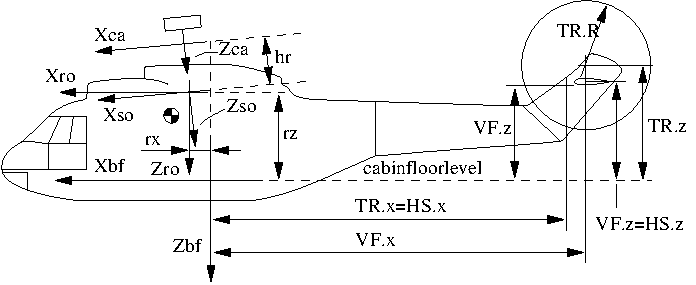
\includegraphics[width=0.7\textwidth]{./figs/chap_introduction/heli_sideview_pdf}
            \else
              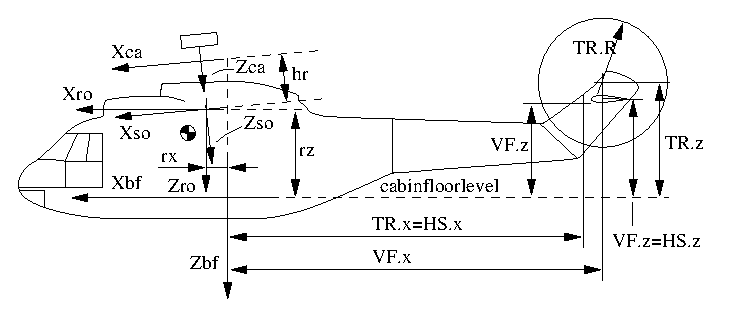
\includegraphics[width=0.7\textwidth]{./figs/chap_introduction/heli_sideview}
            \fi
            \caption[Short caption in the lof: schematic sideview of a helicopter]{Schematic sideview of a helicopter that is by now most likely too long to fit on one line.}
            \label{fig:sideview_reference_frames}
        \end{figure}
        %
%        \begin{figure}[!hbt]
%%             \tiny
%%             \scriptsize
%            \footnotesize
%            \psfrag{Xca}{$\mathsf{X_{hp}}$}
%            \psfrag{Zca}{$\mathsf{Z_{hp}}$}
%            \psfrag{Xro}{$\mathsf{X_{ro}}$}
%            \psfrag{Zro}{$\mathsf{Z_{ro}}$}
%            \psfrag{Xso}{$\mathsf{X_{so}}$}
%            \psfrag{Zso}{$\mathsf{Z_{so}}$}
%            \psfrag{Xbf}{$\mathsf{X_{bf}}$}
%            \psfrag{Zbf}{$\mathsf{Z_{bf}}$}
%            \psfrag{cabinfloorlevel}{$\mathsf{cabin floorlevel}$}
%            \psfrag{TR.R}{$\mathsf{R_{tr}}$}
%            \psfrag{TR.z}{$\mathsf{z_{tr}}$}
%            \psfrag{TR.x=HS.x}{$\mathsf{x_{vf}}$}
%            \psfrag{HS.z}{$\mathsf{z_{hs}}$}
%            \psfrag{VF.z=HS.z}{$\mathsf{z_{hs}}$}
%            \psfrag{VF.z}{$z_{vf}$}
%            \psfrag{VF.x}{$x_{tr} = x_{hs}$}
%            \psfrag{hr}{$h_{r}$}
%            \psfrag{rx}{$r_{x}$}
%            \psfrag{rz}{$r_{z}$}
%            \centering
%            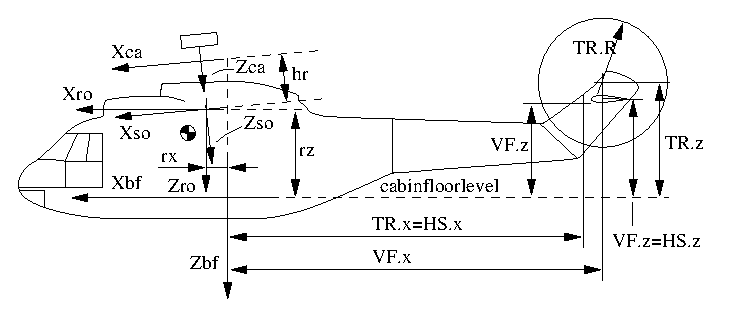
\includegraphics[width=0.7\textwidth]{./figs/chap_introduction/heli_sideview}
%            \caption{Schematic sideview of a helicopter (2)}
%            \label{fig:sideview_reference_frames_2}
%        \end{figure}
        %
        And a fancy figure to show you what is possible with graphics in \LaTeX, see Figure~\ref{fig:blade_geometry}.
        %
%        \begin{figure}[!htb]
%            \centering
%            \subfloat[Equal annuli segment distribution]{%
%                \begin{pspicture}(-0.25,-0.25)(13.125,1.2)
%                    % \psgrid[subgriddiv=1,griddots=10,gridlabels=7pt]
%                    \psdot*[dotsize=4pt](0,0)
%                    % quarter chord line
%                    \psline{-}(-0.25,0)(13.125,0)
%                    % vertical line through centre of rotation
%                    \psline{-}(0,-0.25)(0,0.25)
%                    % blade contours
%                    \pspolygon(3.0625,-0.2363)(13.125,-0.2363)(13.125,0.7088)(3.0625,0.7088)
%                    % blade segment sides
%                    \psline(5.0663,  -0.2363)( 5.0663,  0.7088)
%                    \psline(6.4775,  -0.2363)( 6.4775,  0.7088)
%                    \psline(7.6318,  -0.2363)( 7.6318,  0.7088)
%                    \psline(8.6333,  -0.2363)( 8.6333,  0.7088)
%                    \psline(9.5302,  -0.2363)( 9.5302,  0.7088)
%                    \psline(10.3495, -0.2363)( 10.3495, 0.7088)
%                    \psline(11.1085, -0.2363)( 11.1085, 0.7088)
%                    \psline(11.8190, -0.2363)( 11.8190, 0.7088)
%                    \psline(12.4891, -0.2363)( 12.4891, 0.7088)
%                    % control points
%                    \psdots*[dotsize=4pt](4.0644,  0.0)(5.7719,  0.0)(7.0546,  0.0)(8.1325,  0.0)(9.0817,  0.0)(9.9398,  0.0)(10.7290, 0.0)(11.4637, 0.0)(12.1540, 0.0)(12.8070, 0.0)
%                \end{pspicture}\label{subfig:equal_anulli_distribution}}\\
%            \subfloat[Constant width segment distribution]{%
%                \begin{pspicture}(-0.25,-0.25)(13.125,1.2)
%                    % \psgrid[subgriddiv=1,griddots=10,gridlabels=7pt]
%                    \psdot*[dotsize=4pt](0,0)
%                    % quarter chord line
%                    \psline{-}(-0.25,0)(13.125,0)
%                    % vertical line through centre of rotation
%                    \psline{-}(0,-0.25)(0,0.25)
%                    % blade contours
%                    \pspolygon(3.0625,-0.2363)(13.125,-0.2363)(13.125,0.7088)(3.0625,0.7088)
%                    % blade segment sides
%                    \psline(3.0625,  -0.2363)( 3.0625,  0.7088)
%                    \psline(4.0688,  -0.2363)( 4.0688,  0.7088)
%                    \psline(5.0750,  -0.2363)( 5.0750,  0.7088)
%                    \psline(6.0813,  -0.2363)( 6.0813,  0.7088)
%                    \psline(7.0875,  -0.2363)( 7.0875,  0.7088)
%                    \psline(8.0938,  -0.2363)( 8.0938, 0.7088)
%                    \psline(9.1000,  -0.2363)( 9.1000,  0.7088)
%                    \psline(10.1063, -0.2363)( 10.1063, 0.7088)
%                    \psline(11.1125, -0.2363)( 11.1125, 0.7088)
%                    \psline(12.1188, -0.2363)( 12.1188, 0.7088)
%                    \psline(13.1250, -0.2363)( 13.1250, 0.7088)
%                    % control points
%                    \psdots*[dotsize=4pt](3.5656,  0.00)(4.5719,  0.00)(5.5781,  0.00)(6.5844,  0.00)(7.5906,  0.00)(8.5969,  0.00)(9.6031,  0.00)(10.6094, 0.00)(11.6156, 0.00)(12.6219, 0.00)
%                \end{pspicture}\label{subfig:constant_width_distribution}}
%            \caption[Geometry for a helicopter main rotor blade]{Geometry and segment distributions for a helicopter main rotor blade with 10 segments} \label{fig:blade_geometry}
%        \end{figure}
        %
    \subsection{Alternatives}%
        %
        An alternative to saving figures as PostScript is saving them as PDF. Then, you have to use \emph{pdflatex} which skips the intermediate files. Please note that I will not provide support if you run into problems when you decide to do it this way.
        
        
    % Chapter 1: Introduction
    \chapter{Introduction}
\label{ch:Introduction}

Conventional energy resources such as fossil fuels and nuclear energy are not only limited supply but also pose adhere effects on the environment. Therefore, we are striving to find a cheap and renewable source of energy. Wind energy is such source of energy and is getting more popular, and have also become more affordable. Novel renewable technologies such as Vertical-Axis Wind turbines is now an interested research field.
%\index{VAWT}

\indexAcron{Vertical-Axis Wind Turbine}{VAWT} are unlike the normal wind turbine. Typical wind turbines are mounted on a mast away from the ground and generates energy by spinning normal to the ground. However, a VAWT spins parallel to the ground with its hub located at the ground \cite{website:wikiVAWT}. The advantages of the vertical axis wind turbine are what makes them ideal for a source of renewable energy.  As the turbine is located at the ground, it is easily accessible and can be easily maintained. The second main advantage of the VAWT is the way it dissipates its wake. Near-wake experiments of Ferreira (2009) \cite{Ferreira}, and simulations of Vermeer (2003) \cite{Vermeer2003} have shown that the fluid past the turbine is more turbulent. Due to this higher mixing, the flow is able to smooth out much earlier. This means that it possible to places VAWTs much closer to each other and so a VAWT farm can potentially give more power per area. Furthermore, VAWTs operate independent of the flow direction, and can operate at low wind speeds (low tip-speed ratios).
%\index{HAWT}

However, with these advantages also comes some drawbacks. As the blades passes through its own wake, complex wake-body interactions take places. These have adhere effect on the blade structure and therefore is more susceptible to fatigue. This happens because the blades are constantly pitching, and complex flow behaviour such as dynamic stall and constant vortex shedding occurs \cite{SimaoFerreira2008}. This complex fluid behaviours makes it hard to predict the performance of a VAWT and this is one of the reasons why VAWTs are not mainstream. In addition, as the VAWT operates at large Reynolds number, accurate numerical methods are computationally very expensive. Therefore, it is vital to have a good understanding of the flow structure evolution and the wake generation of the VAWT using not only an efficient method, but also an accurate one.

\section{Motivation and Goal}
The goal of the research is to develop an efficient, reliable, and accurate numerical method for modelling the flow around a 2D VAWT such that one is able to deduce the correct performance characteristics of the VAWT. The two main approaches of investigate the flow is either using a numerical method to simulate the flow or by performing real-life experimental tests.

To understand the unsteady aerodynamic behaviour, \indexAcron{Particle Image Velocimetry}{PIV} has been as useful tool to visualize the flow around the turbine. Ferreira et al. (2007) \cite{Ferreira2007}, have shown that it was possible to acquire flow characteristics around the blade, and these method had the accuracy to be used as validation tools. However, the downside to experimental investigation is that is it very expensive to investigate all types of configuration. Furthermore, the model sizes are limited by the dimensions of the wind tunnel and investigations with arrays of VAWT is difficult.

Numerical methods are a popular alternative as the cost of simulation and the accuracy of the models are increasing day by day. In the research field, there exists many models with various orders of accuracy. \indexAcron{Actuator Disk}{AD} and \indexAcron{Blade Element Momentum}{BEM} models are one of simplest models that are build upon satisfying the momentum balance of the turbine and the fluid. The advantage of theses models are that they are very quick, however they lack the accuracy that can be achieved by experimental simulation. Complex blade-wake interactions such as dynamic stalls and flow separations cannot be modeled by these methods.

	\begin{figure}[!b]
		\centering
		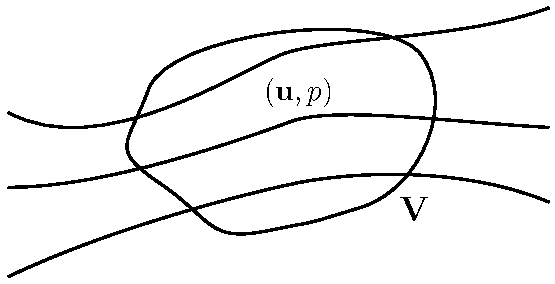
\includegraphics[width=0.4\linewidth]{figures/introduction/eulerianRF.pdf}
		\caption{Eulerian formulation of the fluid. We observe a given volume $\mathbf{V}$ and evaluate the change in properties of the fluid (from incompressible flow: velocity $\mathbf{u}$ and pressure $p$) at time passes.}
		\label{fig:eulerianRF}
	\end{figure}

To ensure more accuracy, one has to solve the Navier-Stokes equation of the flow around the turbine. \indexAcron{Compuational Fluid Dynamic}{CFD} methods discretizes the fluid into smaller regions and solves the set of Navier-Stokes equation in each region (or grids). This type of formulation is known as an Eulerian method as we are evaluating the change in flow property of a given region, figure \ref{fig:eulerianRF}. In order to fully resolve the flow around the turbine, we would have to discretize the fluid at the order of the size of the vortex cores. As the vortex cores are very small (a fraction of size of the airfoil) near the blade, and very large far away from the blade (in order of size of the turbine), we must have grid size that adapts. This requires a large number of grids, as the blades are constantly  moving, and makes it computation very expensive to solve especially for arrays of turbines.

An alternative method is to use the vortex formulation of the Navier-Stokes equations, referred to as vorticity equation. This method is ideal because when describing it in Lagrangian formulation, the vorticity evolution is evaluated as interaction between vortices, and this removes the requirement of gridding, figure \ref{fig:lagrangianRF}. In addition, using simulation acceleration methods such as \indexAcron{Fast Multipole Method}{FMM} and parallel computation in \indexAcron{Graphical Processing Units}{GPU}, they are much more efficient that typical CFD methods and can easily be scaled to distributed computation. However, vortex method cannot inherently take in account the solid body. They require additional methods that can describe the effect of the body in the fluid and the vorticity generated from the body.

	\begin{figure}[!t]
		\centering
		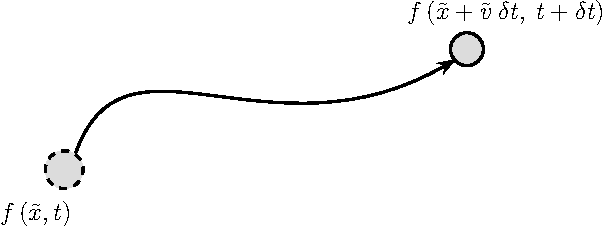
\includegraphics[width=0.4\linewidth]{figures/introduction/lagrangianRF2-crop.pdf}
		\caption{Lagrangian formulation of the fluid. We track the path of the individual fluid elements as time passes.}
		\label{fig:lagrangianRF}
	\end{figure}

So, we see that Eulerian method is accurate when describing the blade-wake interaction but are not efficient when describing multi-scale domains. Whereas, the Lagrangian method is very efficient in evolution the vorticity of the fluid, and is an ideal choice when describing the multi-scale flow characteristics. 

Therefore, in order to use the advantage of both methods, we have decided to use a domain-decomposition method, referred to as \indexAcron{Hybrid Eulerian-Lagrangian Vortex Particle Method}{HVM}. In this method, the Eulerian grid method will be used at the region around the blade (near-wall region). The Lagrangian vortex method will be used in the wake region of the body. With proper coupling of these methods, we can ensure that the this numerical method can capturing not only the near-wake phenomenons such as vortex shedding, dynamic stall, and the wake-body interaction, but also the capture the large-scale flow structures such as the evolution of the VAWT wake, with efficiency and accuracy.

\section{Research Aim and Plan}

\paragraph*{Research Questions:} \textit{Is it possible to develop an efficient and accurate numerical method by an
hybrid approach where the vortex particle method is used in the wake, and the Navier-Stokes grid solver is
used at the near-body region? Will it be able to simulate real life performance characteristics of a vertical
axis wind turbine? Will it be able to predict similar performance characteristics and flow phenomena as observed from the wind tunnel experimental setup? Will it be capable of simulating the blade-wake interaction
and the dynamic stall? Where are the errors and what are their sources?}

\paragraph*{Research aim and plan:}

	\begin{itemize}
	\item Develop the Hybrid method for capturing small-scale phenomenons and large scale phenomenons.
	\item Ensure this tool is efficient, reliable, and accurate.
	\item Verify, Validate the tools with model problems.
	\item Apply the model to the 2D flow of VAWT.
	\end{itemize}

In order to answer this research questions, the goal of the project is the develop an efficient and accurate
numerical method that is not only capable of capture the small scale flow phenomena such as the dynamic stall and the vortex shedding, but is also efficient at modelling the wake evolution of VAWT. The investigation will be performed for 2D geometries and the accuracy of the model needs to established first at simpler problems before continuing to more complex problem cases.

In other words, the initial goal is to develop the hybrid vortex particle method and verify the approach. During this process, the solver will be verified and validated against test cases starting from simpler problems and gradually developing more complex features.

The final goal is to perform a simulation of a VAWT in 2D, compute its performance and validating it against experimental data. By the gradual development of the complex elements of the simulation, one can investigate the feasibility of such approach. Also, the investigation is only done for 2D currently as a full 3D simulation might be difficult and might not be feasible for the master thesis yet.

The innovativeness of this project is that such hybrid modeling has not been yet applied for the wind energy problem case. Through the parallelization of the vortex particle method in a GPU and employing solver acceleration techniques such as the FMM, this simulation could give an edge in the understanding the flow behaviour of a VAWT.

\section{Introduction to Hybrid Eulerian-Lagrangian Vortex Particle Method}

The \indexAcron{Hybrid Eulerian-Lagrangian Vortex Particle Method}{HVM} is a domain-decomposition method, where the Eulerian method and the Lagrangian method solves different domains of the fluid. The domain decomposition method is simply splitting the domain of interest and using the appropriate methods in each domain. For the problem of VAWT, as the boundary is non-trivial and is the source of vorticity, the full Navier-Stokes model will be used here, and away from the body where only the convection of the vorticity field is interested, the fast and efficient vortex particle method will be used, figure \ref{fig:domainDecomposition}.

Several researches have already been done: Cottet and Koumoutsakos (2000a)\cite{Cottet2000a}, Guermond and Lu (2000) \cite{Guermond2000} simulating the advection dominated flows, Ould-Salhi et al. (2001) \cite{Ould-Salihi2001} blending finite difference and vortex method together, Winckelmans et al. (2005a) \cite{Winckelmans2005a} investigating the trailing vorticies, Daeninck (2006) \cite{Daeninck2006} implementing RANS and LES to the simulation, Stock (2010) \cite{Stock} using GPU clusters for efficiency and Speck (2011) \cite{Speck2011a} implementing researching on multipole expansion and modified interpolation kernels.

When evaluating the previous works, we see that not all domain decomposition methods are the same. The main difference differencing between the methods is their coupling strategies. Most works employ the Schwartz alternating method to couple the vortex particle method and the grid solver. The Schwartz alternating method solve the grid solver initially and couples it with the vortex method by iteratively trying to satisfy the boundary conditions. However, for this project the coupling techniques that will be used is similar to Daeninck (2006) \cite{Daeninck2006} and Stock (2010) \cite{Stock}.

	\begin{figure}[!t]
		\centering
		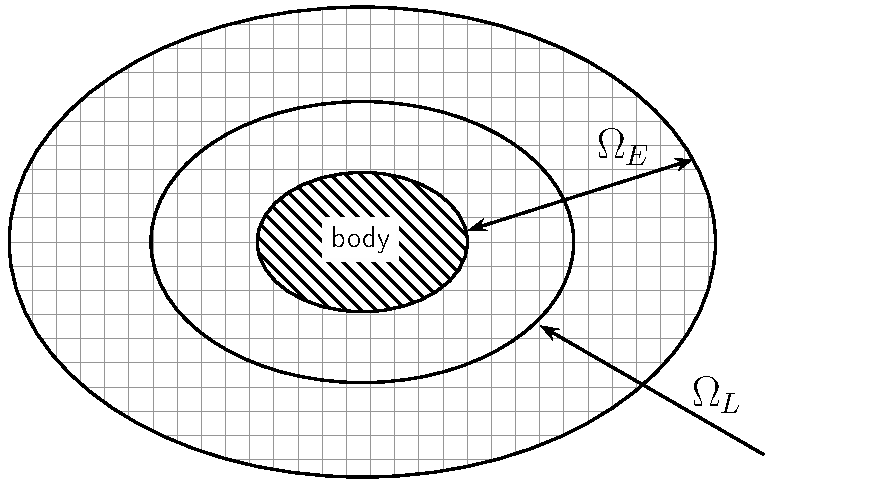
\includegraphics[width=0.5\linewidth]{figures/introduction/domainDecomposition_typical.pdf}
		\caption{Standard domain decomposition using Schwartz iteration for coupling the two methods. Eulerian domain $\Omega_E$ (near the body), and Lagrangian domain $\Omega_L$ (away from the body). Figure is based on Guermond (2000) \cite{Guermond2000}}.
		\label{fig:domainDecomposition}
	\end{figure}

\subsection{Simple coupling strategy}

	\begin{figure}[!b]
		\centering
		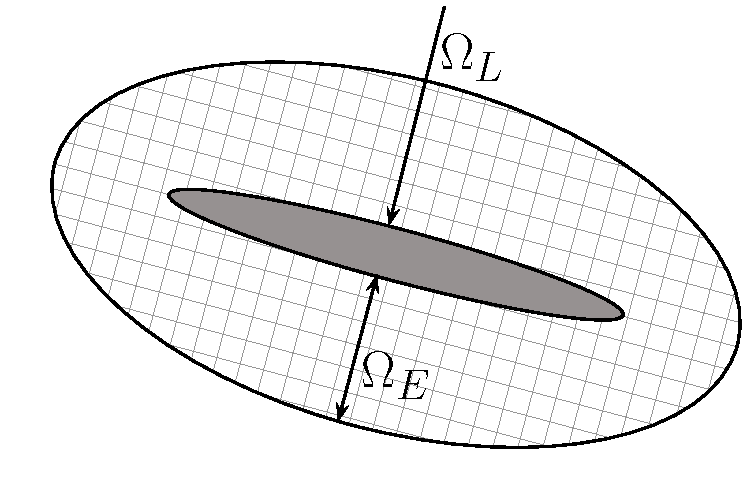
\includegraphics[width=0.5\linewidth]{figures/introduction/domainDecomposition_daenick.pdf}
		\caption{Modified domain decomposition without Schwartz alternating method. Lagrangian domain extends up to the surface of the body. Figure is based on Daeninck (2006) \cite{Daeninck2006}.}
		\label{fig:domainDecomposition_daenick}
	\end{figure}

This new approach is much simpler and only a single iteration is needed for the coupling. The basic procedure is to solve the vortex method in the whole domain using relatively coarse evaluation, then use the grid solver in the near wall region to capture the detailed features of the boundary layer and transfer the vorticity field at this region to the vortex particles, figure \ref{fig:domainDecomposition_daenick}. The functionality of this strategy has been demonstrated by Daeninck and was found to be significantly faster than the Schwartz coupling strategy.

The \underline{features of the simple coupling strategy} can summarized as follows:

	\begin{itemize}
	\item Eulerian method is used to resolve the near-wall region, referred to as Eulerian domain $\Omega_E$. With this implementation, subtle features of the boundary layer (such as flow separation) can be resolved with great accuracy.
	\item Lagrangian method is used to capture the wake, referred to as Lagrangian domain $\Omega_L$. Lagrangian method is used to efficiently evolve the wake.
	\item The accurate solution of the Eulerian domain is transfered to the Lagrangian domain according to the coupling strategies of Daeninck \cite{Daeninck2006} and Stock \cite{Stock}.
	\item The boundary conditions for the Eulerian domain is retrieved from the Lagrangian domain.
	\end{itemize}


	\begin{figure}[!b]
		\centering
		\begin{tikzpicture}
			[node distance=.8cm, start chain=going below,]
			\node[punktchain, join] (correct) {Correct the Lagrangian domain};
		    \node[punktchain, join] (evolveL) {Evolve the Lagrangian solution};
		    \node[punktchain, join] (bcE)     {Determine the Eulerian boundary conditions};
		    \node[punktchain, join] (evolveE) {Evolve the Eulerian solution};
		\end{tikzpicture}
		\caption{Flowchart of the simple coupling strategy. The flowchart shows the procedure to evolve both methods from $t_n$ to $t_{n+1}$.}
		\label{fig:flowchart_simpleCoupling}
	\end{figure}

Figure \ref{fig:flowchart_simpleCoupling} shows the overview to the simple coupling strategy. The detailed algorithm to the simple coupling strategy follows from Daeninck \cite{Daeninck2006}.

The \underline{simple coupling algorithm} can be summarized as follows:

	\begin{enumerate}
	\item \textbf{Correct Lagrangian:} Use the solution of the Eulerian domain $\Omega_E$ (in the near-wall region) to correct the solution of the Lagrangian domain $\Omega_L$ overlapping in the Eulerian domain.  
	\item \textbf{Evolve Lagrangian:} With the modified solution, evolve the Lagrangian solution from $t_n$ to $t_{n+1}$.
	\item \textbf{Determine Eulerian boundary conditions:} Use the Lagrangian solution of $t_n$ and $t_{n+1}$ to determine the boundary conditions of the Eulerian domain.
	\item \textbf{Evolve Eulerian:} With the boundary condition, evolve the Eulerian solution from $t_n$ to $t_{n+1}$.
	\end{enumerate}
	
This is the basic approach for coupling the Eulerian method in the Eulerian domain $\Omega_E$ with the Lagrangian method in the Lagrangian domain $\Omega_L$ without the iterative Schwartz algorithm. In addition, the second difference between the classical hybrid method is that the Lagrangian method handles the boundary conditions differently. Typically during the evolution process of the Lagrangian domain, vorticity is shed from body. However, in this coupling strategy, the Lagrangian method under-resolves the boundary and cannot be used to resolve the vorticity flux. Instead, we use the Eulerian method to resolve the boundary and interpolate the newly generated vorticity into the Lagrangian domain.

However, there as some \underline{assumptions} that we must satisfy, for this coupling strategy to be valid:

	\begin{enumerate}
	\item At $t_n$, before the evolution of both method to $t_{n+1}$, the Lagrangian solution matches Eulerian solution at the near-wall region.
	\item After the evolution to $t_{n+1}$, the deviation of the Lagrangian solution (due to lack of vorticity flux at Lagrangian boundary), is minimal.
	\item Even though the Lagrangian domain is under-resolved in the near-wall region, it should be able to provide accurate boundary conditions for the Eulerian external boundary.
	\end{enumerate}


\section{Verification and Validation Test Cases}

The test-cases that are used for this thesis are summarized as given:

	\begin{description}
	\item[Lamb-Oseen vortex] \cite{Lamb1993} \cite{Tryggeson2007} \hfill\\
	Lamb-Oseen vortex test case is an analytical solution derived from the diffusion equation, and is a test case for unbounded flow (without any wall). This is the first model that will be used to validate the Lagrangian method and Eulerian method separately. This test case focuses on the diffusion of the vortcity is an ideal to verify and validate the convection and diffusion of the vorticity.
	\item[Clercx-Bruneau dipole] \cite{Clercx2006}\hfill\\
	The Clercx-Bruneau dipole test case is the simple case of dipole colliding with a wall and is used to verify the coupling of the methods. This test cases focuses on the generation of vorticity from the wall and is ideal to verify and validate the coupling.
	\item[Impulsively started cylinder] \cite{LEONARD1995} \cite{Chang2006} \cite{Chassaing1986} \cite{Lecointe1985}\hfill\\
	The impulsively started cylinder test case focuses on the forces acting on the cylinder. This test case is used to verify and validate the lift and drag evolution of the cylinder exposed to free-stream flow.
	\item[Elliptic Airfoil] \cite{Nair1997}\hfill\\
	The elliptic airfoil test cases focuses on the flow separation past a lifting body. The elliptic airfoil is pitched at high angle of attack and the flow past the airfoil is comparatively unsteady and undergoes phenomenons such as laminar separation bubble, flow separation and karman vortex shedding from the trailing edge of the airfoil. This helps us ensure coupling process is sound for complex flow phenomenons.
	\end{description}

%\todo{add picture here}
\section{Methodology}
The initial steps of the development of the hybrid vortex methods is as follows:

	\begin{itemize}
	\item Develop the vortex particle method
	\item Validate the vortex particle method against a Lamb-Oseen convection test case.
	\item Develop the vortex panel method to deal with the boundaries for the vortex particle calculation. 
	\item Validate the vortex panel method by solving a potential flow around a cylinder.
	\item Develop the grid solver that is based on the Finite Element method. 
	\item Validate the grid solver against test cases: impulsively starting cylinder, dipole-Wall interaction.
	\end{itemize}

Once all the components have been validated, the methods will be coupled and validated against similar test cases.

	\begin{itemize}
	\item Couple vortex particle, vortex panel and grid solver together.
	\item Validate it with the previous generated test case solution.
	\item Introduce more complicated phenomenons: multiple geometry (i.e multiple grid meshes) and moving boundaries, if it feasible in the constraints of a master thesis.
	\end{itemize}

If the coupled solver has been validated with the test cases, the final step will be to simulated the flow around a VAWT and investigating the performance vs. numerical and experimental data.

%\subsection{Project Plan}

\section{Thesis Outline}

\todo{Update this section}

%\section{Research question}
%\label{sec:ResearchQuestion}
%
%\section{Research objective}
%\label{sec:ResearchObjective}
%
%\section{Importance of study}
%
%\section{Scope of thesis}
%\label{sec:scope}
%
%\section{Structure of the report}
%\label{sec:Structure of the report}

%
	
	%%\documentclass{article}
%
%%\usepackage[pdf]{pstricks}
%\usepackage{hyperref}
%\usepackage{pdfpages}
%
%\title{Project Proposal and Plan}
%\author{Lento Manickathan, 1544101.\\
%Aerodynamics and Wind Energy}
%
%\begin{document}
%\maketitle
%
%\begin{abstract}


%Say very briefly 1) what the project is about, 2) what the main content will be, 3) what the main aim or objectives were, and 4) what the main findings could be. It is nice to end with a strong sentence that highlights the significance of the work to be undertaken and any long-standing contribution to the body of knowledge. Remember that this is a proposal of work to be done and so you might also say something about the motivation and feasibility.


%
%\end{abstract}

\chapter{Project Plan}
%\label{sec:intro}

%Introduce the general area of interest of the project, setting out any advancements and challenges of interest. What is the relevance of the work at an academic and applied/industry level? Then introduce more fully the specific investigation addressed in the project proposal and perhaps even set out the main goal of the work (Note: different to the research question!). Say very briefly what is then to come in the layout of the proposal. Note: the intro should include general references to back up the points made.

%We, the humankind, are now facing several challenges in finding a cheap and reliable energy source. Conventional energy resources such as fossil fuels and nuclear energy are not only limited supply but also pose adhere effects on the environment. Therefore, we are striving to find a cheap and renewable source of energy. Wind energy is such source of energy and is therefore getting more popular and also become more affordable and novel renewable technologies such as Vertical-Axis Wind Turbine (VAWT) is now an interested research field.\\
%
%Vertical-Axis Wind turbine or VAWTs are unlike the normal wind turbine. Typical wind turbines are mounted on a mast away from the ground and generates energy by spinning normal to the ground. However, a VAWT spins parallel to the ground with its hub located at the ground \cite{website:wikiVAWT}. The advantages of the vertical axis wind turbine are what makes them ideal for a source of renewable energy.  As the turbine is located at the ground (unlike the Horizontal-Axis Wind Turbine), it is easily accessible and can be easily maintained. The second main advantage of the VAWT is the way it dissipates its wake \cite{Ferreira} \cite{Vermeer2003}. As the fluid past the turbine is more turbulent, the flow is able to smooth out much earlier. This means that it possible to places VAWTs much closer to each other is so in future this means that a VAWT farm can potentially give more power per area. Furthermore, operate independent of the flow direction and can operate at low wind speeds (low tip-speed ratios).\\
%
%However, with these advantages also comes drawbacks. As the blades passes through its own dirty air (the wake), complex wake-body interactions take places. These have adhere effect on the blade structure and therefore is more susceptible to fatigue. This happens because the blades are constantly pitching in front the free-stream flow and complex flow behaviour such as dynamic stall and constant vortex shedding occurs \cite{SimaoFerreira2008}. This complex fluid behaviours makes it hard to predict the performance of a VAWT and this is one of the reasons why VAWTs are not mainstream. In addition, as the VAWT operates at large Reynolds number, accurate numerical methods are computationally very expensive. Therefore, it is vital to have a good understanding of the flow structure evolution and the wake generation of the VAWT using not only an efficient method, but also an accurate one.\\
%
%They key interest of this project is the develop a efficient, reliable and an accurate fluid dynamics solver for the modelling the flow around a 2D VAWT. This numerical tool should not only be accurate at capturing the small scale phenomenons such as vortex shedding, dynamic stall and wake-body interaction, but should be efficient at capturing the large scale phenomenons such as the wake evolution of the VAWT. This is one of the main challenges of this project because if one is interested in the phenomena of one scale, it will compromise the other. Therefore, one of the main goals of the project will be accurate development of method and for modelling fluid around multiple moving geometries of non-trivial shapes. To verify the accurate implementation, various benchmark cases will be investigated and finally will be validated against numerical and experimental data of VAWT.
%
%To overcome this dilemma, we are going to employ a hybrid numerical method which couples the accurate Navier-Stokes grid solver near the body and the efficient vortex particle method at the domain away from any boundaries. This hybrid vortex particle method, will be not only be able to capture the small scale phenomenons of the boundary but can also be enabled to be parallelized making ideal in understand the multiple wake-body interactions and computation of large-scale phenomenons of wind farms. Such methodology has been already been investigated \cite{Daeninck2006} \cite{Cheng1997} \cite{Ould-Salihi2001} \cite{Zhao2007} \cite{Stock}, however has yet not been used for VAWT problem.\\

The main goal of the project is to develop an efficient and accurate numerical method to simulate the complex flow phenomenons of a Vertical-Axis Wind Turbine. To achieve this goal, the project will be focused on developing a hybrid vortex method by coupling a Finite Element grid solver in the near-wake domain and the vortex particle method in the far-wake domain. The challenge arise from the domain decomposition of the Eulerian grid solver and the Lagrangian particle method. Several test cases such as dipole-Wall interactive and flow around a cylinder, aerofoil with be used to verify and validate the accuracy of the model. By accurately capturing the boundary layer phenomenons such as flow separation and dynamic stall with the grid solver, and efficiently modelling the wake using vortex particles, the numerical model is ideal for evaluation complex flow phenomenons of multi-body wing energy problems wake-body interaction and is also ideal to model very-large scale complex problems such as Vertical-Axis Wind Turbine farms.


\section{State of the art}
%\label{sec:litreview}

%This is a detailed part of the proposal that rigorously reviews what work has been already carried out by other academics in this area while also benchmarking industry best practice. The researcher is trying to establish: 1) what research areas are relevant, and 2) what the current understanding is along with any opposing views. It is very nice to end with some sort of synthesis of the presented State-of-the-art to link explicitly to the work in the proposal, especially with regard to the following Section. This might even include a statement of what the author sees their work adding to the body of knowledge.

To understand the flow behaviour of a VAWT, several numerical research \cite{Almohammadi2013} \cite{Ferreira2007} \cite{Islam2008} \cite{Merz2012} and experimental researches \cite{SimaoFerreira2008} \cite{Ferreira} \cite{Howell2010} \cite{Mertens2003} have been undertaken.\\

To understand the unsteady aerodynamic behaviour, the dynamic stall, experimental tools such as Particle Image Velocimetry (PIV) have been a popular choice, see Ferreira et al. (2007) \cite{Ferreira2007}. In order to evaluate the flow numerically in an accurate fashion, they have used various grid-solvers with turbulence models such as such as URANS, LES and DES. Similar numerical investigation has also been applied by Almohammadi et al. (2013) \cite{Almohammadi2013} for a straight blade VAWT in 2D. However, these models are computationally very expensive.\\

Researches have also been done in less expensive, simpler tools such as blade momentum models by Islam et al. (2008) \cite{Islam2008}, a more accurate tools such as multiple streamtube model and it is also possible to model the flow using vortex methods. These methods are the simplification of the Navier-Stokes models using assumptions such as inviscid flow (valid for large Reynolds number). However, the downside to such models is that they cannot accurately capture the near-body phenomenons such as the vortex shedding, which has considerable impact on the performance characteristics of the VAWTs.\\

However, all the numerical method that was grid-based struggled with dealing with large number of mesh cells for high Reynolds numbers and the numerical method that employed simplified Navier-Stokes methods had to sacrifices some accuracies. The experimental investigation also come with drawbacks as they are require more financial resources and are only feasible to model the small scaled VAWTs.\\

This is the main advantage and the relevance of the hybrid vortex particle method for the research in VAWT. As computers are getting more powerful and less expensive, the computational research is becoming more popular. By utilizing the two methods together, the vortex particle method away from body, and the Navier-Stokes solver with the turbulence model in the near-body region, one will be able to tackle the challenges in an efficient manner.\\ 

In the field of hybrid methods that couples the Navier-Stokes solver and the vortex particle methods, various approaches can be taken. There are two main types of coupling: the Vortex-in-Cell method (VIC) and the domain decomposition method. The VIC methods employs both the methods in the same domain. The vortex method is used to solve for the velocity field using a fast poisson evaluations, and the grid-solver is used to solve the diffusion terms. Such methods have been previously used by Ould-Salihi et al. (2001) \cite{Ould-Salihi2001}. However, VIC is only ideal in the confined domains because a mesh formulation is needed for the full domain. This is why domain decomposition is useful for simulation the flow of the VAWT. The grid solver is only used to solve the flow near the body and is then coupled with the vortex particles methods, which efficiently solves the vorticity field in the off-body region. Such methods have be applied by Winckelman et al. (2005a) \cite{Winckelmans2005a} and Daeninck (2006) \cite{Daeninck2006}.\\ 

For solving the near-body domain, Ould-Salihi et al. (2001) \cite{Ould-Salihi2001} have used Finite Difference Method, Stock 2010 \cite{Stock} has used the OVERFLOW package and Guermond and Lu (2000) \cite{Guermond2000} a Finite Element formulation. Extensive investigation of the vortex methods have been lay down by Cottet and Koumoutakos \cite{Cottet2000a} and various further researches have been done on this topic by Ghoniem et al. \cite{Sethian1988} \cite{Lakkis2009} using adaptive vortex method, Beale and Majda \cite{Beale1985}, researcing on the vortex kernels and Leonard \cite{Couet1981} implementing the strategy to 3D flows.\\

\section{Research question, aims and objectives}
%\label{sec:objective}

%What is the main research question to be solved in reaching the project goal? There can be more than one but be focused. These research questions should be very precise and almost like a requirement, be unambiguous, unique, measurable, and answerable in a meaningful way. 

%The objective then is basically the project goal, again clearly stated in terms of what the researcher wants to achieve, and by which means you will achieve this. This is then followed by tangible sub-goals that will be necessary to make this happen. These sub goals can then be developed into task blocks in the project plan/Gantt chart.

% Make the novelty and innovation clear!

%Again, remember that this is a proposal of work to be done and so you might also say something about the motivation and feasibility.

The main research question is: Is it possible to develop an efficient and accurate numerical method by an hybrid approach where the vortex particle method is used in the wake, and the Navier-Stokes grid solver is used at the near-body region? Will it be able to simulate real life performance characteristics of a vertical axis wind turbine? Will it be able to predict similar performance characteristics and flow phenomena as observed from the wind tunnel experimental setup? Will it be capable of simulating the blade-wake interaction and the dynamic stall? Where are the errors and what are their sources?\\

In order to answer this research questions, the goal of the project is the develop an efficient and accurate numerical method that is not only capable of capture the small scale flow phenomena such as the dynamic stall and the vortex shedding, but is also efficient at modelling the wake evolution of VAWT. The investigation will be performed for 2D geometries and the accuracy of the model needs to established first at simpler problems before continuing to more complex problem cases.\\

In other words, the initial goal is to develop the hybrid vortex particle method and verify  the approach. During this process, the solver will be verified and validated against test cases starting from simpler problems and gradually developing more complex features.\\

The final goal is to perform a simulation of a VAWT in 2D, compute its performance and validating it against experimental data. By the gradual development of the complex elements of the simulation, one can investigate the feasibility of such approach. Also, the investigation is only done for 2D currently as a full 3D simulation might be difficult and might not be feasible for the master thesis yet.\\

The innovativeness of this project is that such hybrid modelling has not been yet applied for the wind energy problem case. Through the parallelization of the vortex particle method in a GPU and employing solver acceleration techniques such as the Fast Multi-pole Method (FMM), this simulation could give an edge in the understanding the flow behaviour of a VAWT.


\section{Theoretical Content/Methodology}
\label{sec:theory}


%What is the theoretical basis of the work to be undertaken? Is there a hypothesis to be tested? Are a couple of theoretical approaches going to be used together in a hybrid approach. What are the steps to be undertaken in the project - linking to the objectives established in Section~\ref{sec:objective}.

If this research has a hypothesis, then it is that is the hybrid vortex particle method for simulation a flow around a VAWT is efficient, accurate and feasible. Therefore, in order to verify this hypothesis, the main work in this project will the development of the numerical tool and then investigating its performance against appropriate test cases.\\

The ground work for the hybrid vortex method have been previously been investigated by Cottet and Koumoutakos \cite{Cottet2000a}. Daeninck has shown in his work that this approach can easily be scaled to 3D geometries \cite{Daeninck2006} and is therefore possible to simulate a full VAWT. Stock has shown that parallelization of the hybrid vortex method is possible \cite{Stock}.\\

Furthermore, a standard vortex method have already been implemented for simulating the flow by Ferreira \cite{Ferreira} and have also shown that grid solver is able to capture the near-wake phenomenons \cite{SimaoFerreira2008}. Thus, it is feasible to use a hybrid vortex method for simulation a VAWT.

\subsubsection*{Methodology}

The initial steps of the development of the hybrid vortex methods is as follows:

\begin{itemize}
\item Develop the vortex particle method
\item Validate the vortex particle method against a Lamb-Oseen convection test case.
\item Develop the vortex panel method to deal with the boundaries for the vortex particle calculation. 
\item Validate the vortex panel method by solving a potential flow around a cylinder.
\item Develop the grid solver that is based on the Finite Element method. 
\item Validate the grid solver against test cases: impulsively starting cylinder, dipole-Wall interaction.
\end{itemize}

Once all the components have been validated, the methods will be coupled and validated against similar test cases.\\

\begin{itemize}
\item Couple vortex particle, vortex panel and grid solver together.
\item Validate it with the previous generated test case solution.
\item Introduce more complicated phenomenons: multiple geometry (i.e multiple grid meshes) and moving boundaries, if it feasible in the constraints of a master thesis.
\end{itemize}

If the coupled solver has been validated with the test cases, the final step will be to simulated the flow around a VAWT and investigating the performance vs. numerical and experimental data.\\

\section{Experimental Set-up}
\label{sec:experiment}

%What is your laboratory set-up or in the field set-up, presented so readers can better informed and critical of any limitations etc of your research environment and set-up, etc. For example, how will the collaboration with industry work or otherwise what are any practical implications of your Methodology from Section~\ref{sec:objective}?Experiments are more then just questionnaires, interviews or physical tests in a laboratory. Programming and computer modeling are also considered experiments sop their set up and limitations can also be discussed here.

The setup of the numerical simulation can be summarized to the test cases and the final VAWT problem. All of the numerical investigations is done for a 2D case and it is vital to establish the feasibility of the model before continuing to more complex ones.\\

To validate the vortex particle method, the Lamb-Oseen test case will be used. The vortex particle used blobs that carry the approximate the vorticity field. These blobs are then convected and diffused using the Biot-Savart Law  \cite{Cottet2000a}, and are diffused using appropriate diffusion models \cite{Wee2006}. The Lamb-Oseen test case is a standard benchmark case for validating the vortex method and it deals with the diffusion of the viscous vorticity field \cite{Shankar1996} \cite{Speck2011a} \cite{Barba2004a}. To efficiently calculate the convection, the model will be written in Python scripting language due to its high modularity and its large collection of open source libraries. This will enable the use of parallelization of Biot-Savart evaluation in NVIDIA CUDA platform using FMM.\\ 

The grid solver will be written using the FEniCS open source libraries for Finite Element computation. Their libraries is accessible to python scripting and can therefore be easily be used to couple to the vortex method. To validate the FEM solution, a collision of dipole to a no-slip boundary will be investigated. This is not only helpful in validating the FEM but also can later be used to validate the coupled model as problem case uses simple geometries. Such investigations have been recommended for vortex method by Renac et al. (2013) \cite{Renac2013} and Clercx and Bruneau (2006) \cite{Clercx2006}. These literature will be used to validate the results of the FEM simulations.\\

The experimental set-up for coupled case is impulsively started cylinder. The cylinder is submerged into unperturbed flow and the vorticity evolution is investigated to validate the numerical method. Similar investigations have been done by Issam and Ghoniem (2009) \cite{Lakkis2009}, Cheng et al. (1997) \cite{Cheng1997}, Guermond and Lu (2000) \cite{Guermond2000} and Rossinelli et al. (2010a) \cite{Rossinelli2010a}. Again, these results will be used to validate the results of the coupled model.\\

In the end, the flow of a VAWT will be simulated and the experimental data from Ferreira \cite{Ferreira} \cite{Ferreira2007} \cite{SimaoFerreira2008}, together with the numerical results will be used to evaluate the variation is the results generated by the hybrid method.\\

\section{Results, Outcome and Relevance}
\label{sec:result}

%What data etc will you be working with, which variables and parameters, and what type of results do you want to investigate. Then go on to try and project the sort of outcome you are interested in and of course ultimately what the relevance of that is. 

The output data of all the simulation will the primitive variables of the Navier-Stokes equations: velocity and pressure. These results will be used then to post-process and calculate the vorticity field of the flow of VAWT. This, is useful as a direct comparison with the vorticity evolution of the VAWT can be done. Moreover, further results such as the time averaged flow field, the variation in the angle of attack, the variation in the induction field, the evolution of the shed vorticity, the time-averaged vorticity density distribution and the time-averaged velocity induction field due to the wake can be investigated. From here, the performance of the VAWT can be investigated and in future, the power generation of the VAWT can be analyzed.\\

This is why the hybrid vortex method is relevant. As the simulation is more accurate and comparatively much faster than other models, it will be capable of generating performance data and insightful investigation of the impact of a given design parameter can be done.\\

The deliverable of the thesis will be the coupled hybrid-vortex particle method that is capable of simulating a flow around a VAWT. Together with this, a detailed report will be handed containing the verification and the validation done for the numerical tool. In conclusion, the hypothesis whether it is feasible to use a hybrid vortex method for simulating a VAWT will be answered.\\


\section{Project Planning and Gantt Chart}
\label{sec:planning}

%Look at the logistics of carrying out the work, develop the intended work into work packages (from the tasks say mentioned in Section~\ref{sec:objective}) and then incorporate all that into a schedule of work through a Gantt chart (or Integrated Master Plan/Integrated Master Schedule). You must at a reasonably high level try to estimate time required and any resource constraints etc and then fit that into a schedule. A Work Breakdown Structure and Work Flow Diagram can be very helpful (ref: DSE). You will put in three key review points: 1) the Kick-off Review; 2) the Mid-term Review; and 3) the Green Light Review. Remember holidays etc, preparing deliverables etc and that some tasks will be concurrent, running in parallel. Finally, the Gantt should visibly show any key review points, milestones (points of specific achievement relative to the end goal) and deliverables (tangible outputs such as reports, presentations, papers, manuals, tools, workshops, etc).

The work that has been proposed here should be feasible for a master thesis project extending for a period of 9 months.
The intended work can be divided into 3 main packages. In the initial work schedule involves the thorough research of all the topics related to be done. In this phase, the problem will be thoroughly explored identifying and establishing all the proper choices that needs to be made. For example, the diffusion of the vortex particle can be done in several schemes and during this phase an appropriate choice will be made using careful scrutinizing. Other overhead work such as arranging the work breakdown and thorough planning of the thesis will be discussed with the supervisors. Finally, this phase will be finalized with a kick-off meeting, presenting the findings and discussing the through plan of the next phase.\\

The second phase is the key phase of the thesis, as this is where the main work will be done, see figure \ref{fig:FlowChart}. The work that will be undertaken is as discussed before, where the conclusion of the literature study is be used to develop, verify and validate the numerical method. Throughout this phase, several mid-term reports will be handed in concluding the finding each of the sub researches. This phase will be done reach the conclusion when the full 2D simulation of the VAWT is reached and finally validation versus numerical and experimental data provided from Ferreira \cite{SimaoFerreira2008}. \\
 
\begin{figure}[htp]
\centering
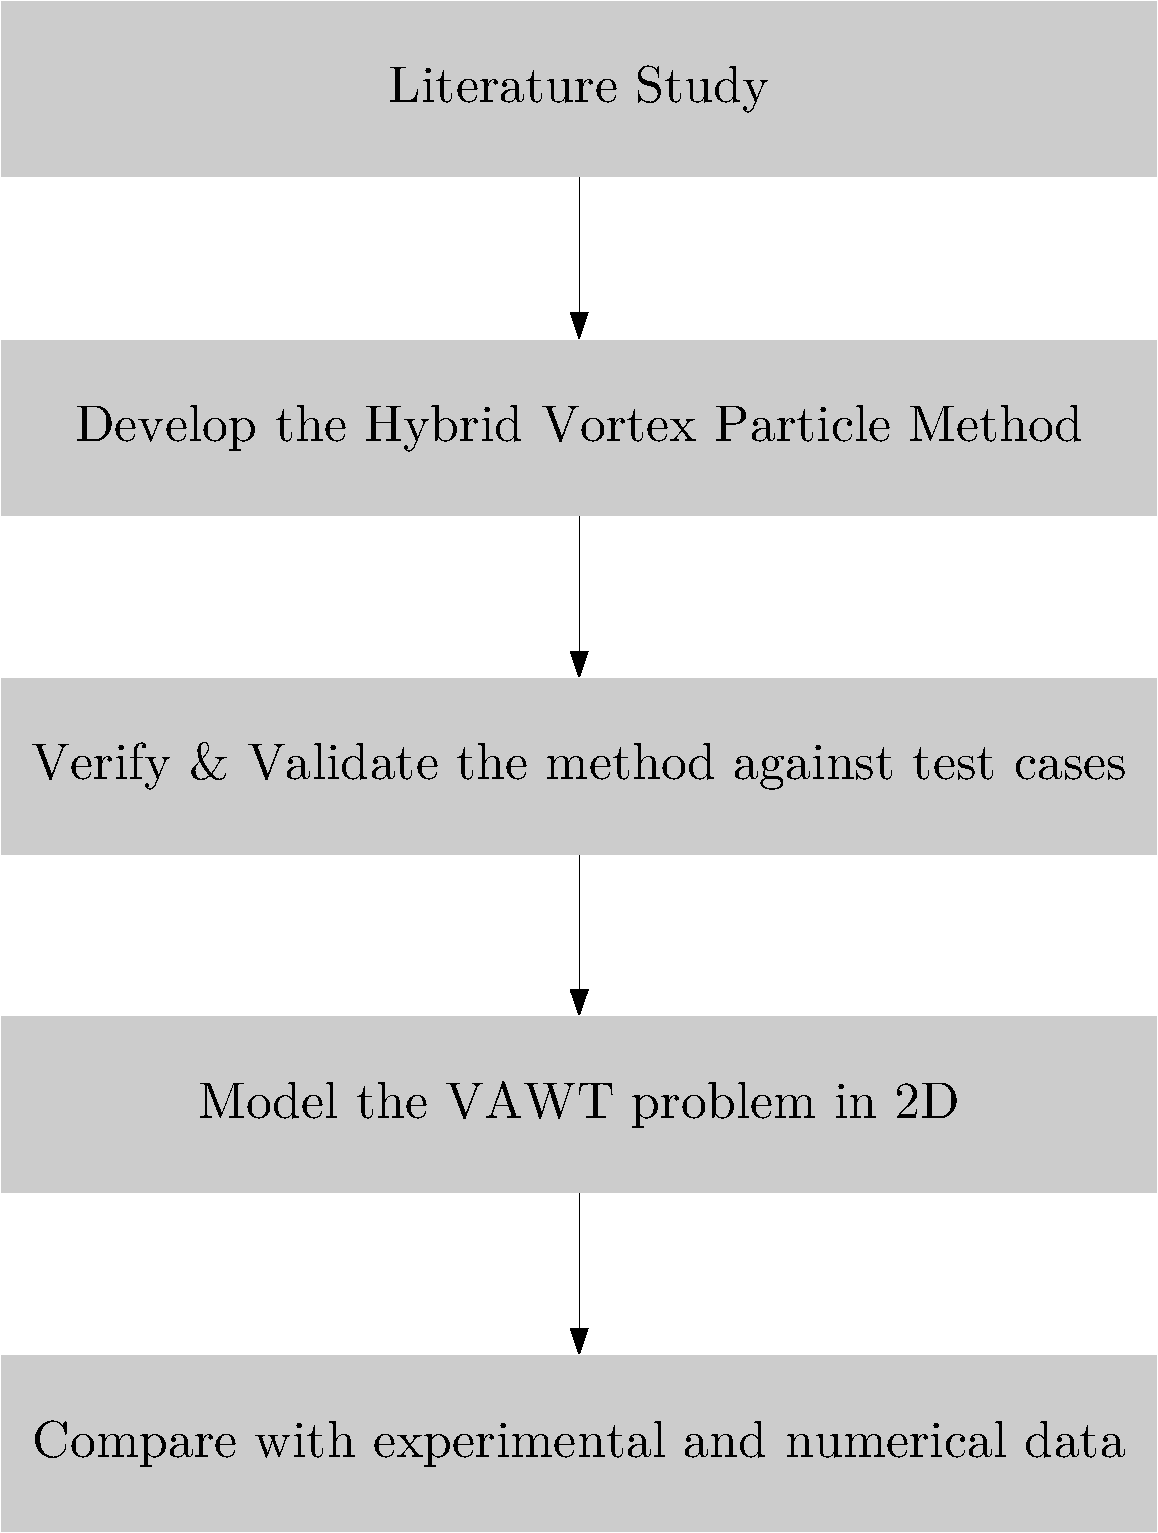
\includegraphics[scale=0.3]{figures/FlowChart.pdf}
\caption{The simplified work breakdown structure of the thesis}
\label{fig:FlowChart}
\end{figure}

The final phase is initiated by the preparation of the draft report. This report will include the verification and the validation of the work and will be carefully discussed with the supervisors. Once the green light if given, the project will be concluded with the request for examination data, submitting the documents and preparation for the graduate presentation. A detailed schematic of the thesis work can be investigated in the gantt chart \ref{fig:GanttChart}.\\

\begin{figure}[p]
\centering
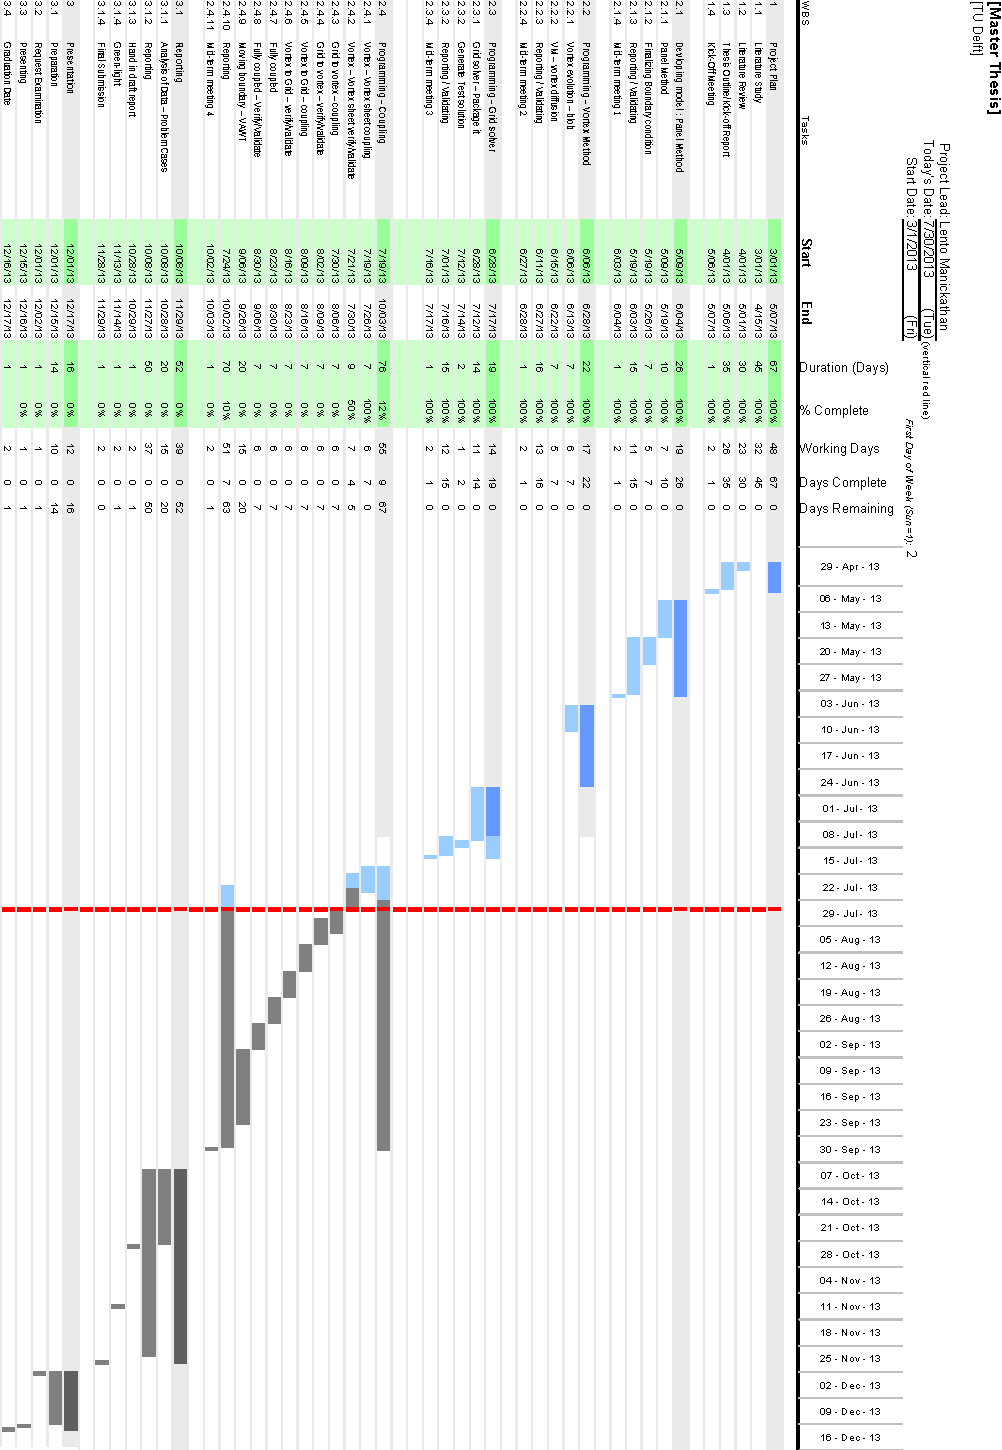
\includegraphics[scale=0.75]{figures/GanttChart.pdf}
\caption{Detailed Gantt chart of the thesis}
\label{fig:GanttChart}
\end{figure}

\newpage

\section{Summary of Project}
%\label{sec:conclusions}

%The conclusions regarding what you are proposing should be written in a precise, unique, clear and accurate manner. Always check if they are well supported by the work you presented in the paper and check them against the main literature so that you can make a statement about the longer-term impact of your work on the body of knowledge? Lift the most important conclusions into the Executive Summary and check that both are consistent, also with the Introduction as the Executive Summary, Introduction and Conclusion form the key points of entry and exit into the work and make a big impact on accessibility and getting across the relevance!

In conclusion, this thesis will be focused on developing an efficient and accurate numerical method to simulate the complex flow phenomenons of a Vertical-Axis Wind Turbine.\\

During the initial stages, a strong theoretical basis will be established before reaching the main development process. During this stage, the innovativeness of the method will be established. The main work will the development of the tool, its verification and the validation against the test cases: dipole-wall interaction, impulsively starting cylinder, multiple geometries, and finally simulating the moving geometry. Concise mid-term reports will be handed once the validation of each of the components is done so that a detailed conversation can me maintained with the supervisor and if possible publishing the results. Before reaching the final stages, the draft report will be made to have ensure smooth transition to the graduation.\\

%\newpage
%
%\bibliographystyle{plain}
%\bibliography{../library}

%List all references consistently, using one of the preferred approaches. The key thing is that the referred to author is given credit through their earlier work, that this is dated to show the chronological order of developments, and that the reader has enough information to go and find that specific reference. Relative to the latter point: where was the conference and did the proceedings have an ISBN number; or if a book what is the ISBN number and publisher, or if a journal paper what was the volume or edition number and certainly page number. The strongest references are ones that have been reviewed prior to publication (journals for example) and the weakest are web sites and popular publications. Only reputable websites (from a society or major industry player) should be included and the date of access should be noted. If at all possible stay away from web references as they are so uncontrolled as sources of information.

%\LaTeX {} template based on \cite{template}.

%\end{document}
	
    % Chapter 2 : Literature Review
    %\chapter{Literature Review}
\label{ch:LiteratureReview}

%This is a detailed part of the proposal that rigorously reviews what work has been already carried out by other academics in this area while also benchmarking industry best practice. The researcher is trying to establish: 1) what research areas are relevant, and 2) what the current understanding is along with any opposing views. It is very nice to end with some sort of synthesis of the presented State-of-the-art to link explicitly to the work in the proposal, especially with regard to the following Section. This might even include a statement of what the author sees their work adding to the body of knowledge.

%%%%%%%%%%%%%%%%%%%%%%%%%%%%%%%%%%%%%%%%%%%%%%%%%%%%%%%%%%
\section{Current approaches}

\subsection{Momentum Theory}

\subsection{Single/Multiple Streamtube Model}

\subsection{Vortex Theory}

\subsubsection{Vortex Filament/Lifting Line Theory}

\subsubsection{Vortex particle Method}

\subsection{Full Navier-Stokes Model}

%%%%%%%%%%%%%%%%%%%%%%%%%%%%%%%%%%%%%%%%%%%%%%%%%%%%%%%%%%
\section{Purpose of further research}


%%%%%%%%%%%%%%%%%%%%%%%%%%%%%%%%%%%%%%%%%%%%%%%%%%%%%%%%%%
\section{Relevant research areas}

%\subsection{Domain decomposition methods}
%
%\subsubsection{Coupling techniques}
%
%\subsection{Simulation acceleration techniques}
%\section{Former Work}
%\label{sec:FormerWork}
%
%\subsection{Overview of the Work}
%\label{subsec:OverviewoftheWork}

%\section{Purpose of further research}

%%%%%%%%%%%%%%%%%%%%%%%%%%%%%%%%%%%%%%%%%%%%%%%%%%%%%%%%%%%%%%%%%%%%
%\nomenclature[ak]{$K$}{Kelvin (temperature)}
%\nomenclature[ar]{rpm}{Revolutions per minute (frequency)}
%\nomenclature[ac]{CO}{Carbon Monoxide}
%\nomenclature[ac]{CRM}{Chemical Reaction Modelling}
%\nomenclature[ah]{H2}{Molecular hydrogen}
%\nomenclature[ag]{GSP}{Gas Turbine Simulation Program (Software)}
%\nomenclature[rr]{$\rho$}{Density \nomunit{[$kg/{m^3}$]}}
%\nomenclature[sm]{$\dot{m}$}{Mass flow rate \nomunit{[$kg/s$]}}
%\nomenclature[ab]{bar}{Pressure}

%\nomenclature[rr]{$Re$}{Reynolds number \nomunit{[-]}}
%\nomenclature[rw]{$M$}{Mach number \nomunit{[-]}}
%\nomenclature[rw]{$\mu$}{Dynamic viscosity of air \nomunit{[$kg/{s \cdot m}$]}}
    \chapter{Theory on Vortex Particle Method}
\label{ch:theory}

To model the flow around a VAWT, several approaches can be taken, Vermeer at al. (2003) \cite{Vermeer2003} have also summarized in their paper. The two main approaches of investigating the flow is either employing a numerical method to simulate the flow or through experimental simulations.

Leishman (2006) \cite{leishman2006principles} has shown that there are several simplified, efficient numerical tools that can be used to model the performance of a VAWT. Methods such as actuator disk theory and blade element momentum theory and deals with simplified Navier-Stokes equations and is very useful to evaluate the trend of certain design parameter. However, as they are highly simplified, complex flow phenomenons that has severe impact of the performance characteristics of the VAWT such as flow separation during dynamic stall, vortex shedding during the rotation and blade-wake interaction cannot be simulated. In order to understand them, either experimental investigation such as in wind tunnel or full Navier-Stokes simulations have to undertaken. So to understand the flow behaviour of a VAWT, several numerical research have been performed \cite{Almohammadi2013} \cite{Ferreira2007} \cite{Islam2008} \cite{Merz2012} and experimental researches by Ferreira \cite{SimaoFerreira2008} \cite{Ferreira} and others \cite{Howell2010} \cite{Mertens2003}.

All the numerical method that was grid-based struggled with dealing with large number of mesh cells for high Reynolds numbers and the numerical method that employed simplified Navier-Stokes methods had to sacrifices some accuracies.The experimental investigation also come with drawbacks as they are require more financial resources and usually only feasible to model the scaled VAWTs.

This is the main relevance of the hybrid vortex particle method for the VAWT investigations. By utilizing the two methods together, the vortex particle method away from body, and Navier-Stokes solver with turbulence model in the near-body region, one will be able to tackle the challenges in an efficient manner.

Therefore, this chapter is dedicated to given an overview on the theory of the Vortex Particle Method which we will employ with coupled Navier-Stokes solver. 

\textcolor{red}{!! Add chapter outline here !!}

\section{Governing Equation of Vortex Method}

Vortex methods deals with the evolution of the vorticity field in the fluid domain \cite{Cottet2000a}. So to derive the governing equations of 2-D \printAcron{Vortex Particle Method}{VPM}, we must examine the 2-D incompressible Navier-Stokes equations of a viscous fluid flow. The momentum equation is given as

%(\textcolor{darkblue}{VPM})
%\newcommand{\printAbbreviation}[3]{#1 (#2) \nomenclature[#3]{#2}{#1}}
%\nomenclature[av]{VPM}{Vortex Particle Method}
%\printAbbreviation{Vortex Particle Method}{VPM}{av}
%\acron[t]{VPM}{Vortex Particle Method}

\begin{equation}
\frac{\partial \mathbf{u}}{\partial t} + \mathbf{u}\cdot\nabla\mathbf{u} = - \frac{1}{\rho} \nabla p + \nu \nabla^2\mathbf{u},
\label{eq:mom}
\end{equation}

with $\zeta$ characterizing the distribution of the vorticity, where $\mathbf{u}\left(\mathbf{x},t\right)$ \lsymb[f]{$\mathbf{u}$}{Velocity vector}{$[m/s]$}{u} describes the velocity field of the fluid domain, $p\left(\mathbf{x},t\right)$ \lsymb[f]{$p$}{Pressure}{$[\mathrm{Pa}]$}{p} describes the pressure field, and \gsymb[t]{$\nu$}{Kinematic viscosity}{$[m^2/s]$}{mm} and \gsymb[t]{$\rho$}{Density}{$[kg/m^3]$}{qq} are the kinematic viscosity and the density of the fluid respectively. We also have to satisfy the incompressiblity constraint given as

\begin{equation}
\nabla\cdot\mathbf{u} = 0.
\end{equation}

The governing equation of the VPM is vorticity-velocity formulation of the fluid domain. Vorticity  \gsymb[t]{$\omega$}{Vorticity}{$[1/s]$}{xx} is defined as

\begin{equation}
\mathbf{\omega} = \Delta \times \mathbf{u},
\end{equation}

and so by taking the curl of the momentum equation, we derive the vorticity transport equation, 

\begin{equation}
\frac{\partial \omega}{\partial t} + \mathbf{u}\cdot\nabla\omega = \nu \nabla^2 \omega.
\end{equation}

The VPM deals with the evolution of the vorticity feild using the viscous splitting (or Fractional step) method \cite{Cottet2000a}. The time stepping of the vorticity is done by dealing the viscous and the inviscid part of the transport equation separately,

\begin{itemize}
\item convection:
\begin{equation}
\frac{\partial\omega}{\partial t} + \mathbf{u}\cdot\nabla\omega=0;
\label{eq:convectionEulerian}
\end{equation}
\item diffusion:
\begin{equation}
\frac{\partial\omega}{\partial t} = \nu\nabla^2\omega.
\end{equation}

\end{itemize}

The first substep of the evolution deals which the convection of the vorticity. The diffusion of the vorticity field is evaluated by modifying the vorticity field after the convection. 
%This equation is known as the vorticity transport equation \cite{LEONARD1995}. To solve this equation, we employ a viscous splitting algorithm, where the evolution of the vorticity field is convection and the diffusion of the vorticity field is handled in separate sub-steps.

%There are several advantage to this type of evolution. As the convection and diffusion are handled separately, there is minimum dispertion during the convection and furthermore, the is no restriction of the advection CFL number \cite{Wee2006}.


\section{Spatial discretization: Generation of vortex blobs}

The spatial discretization of the fluid domain is done by representing the vorticity field in $N$ Lagrangian vortex particles. This is done by dividing the fluid domains into cells where the circulation of the region is assigned to the particle. This gives 

\begin{equation}
\omega\left(\mathbf{x},t\right) \simeq \omega^h\left(\mathbf{x},t\right) = \sum_{p}\Gamma_p\left(t\right)\zeta_{\sigma}\left[\mathbf{x}-\mathbf{x}_p\left(t\right)\right],
\end{equation}

where $\Gamma_p$ \gsymb[f]{$\Gamma$}{Circulation}{$[m^2/s]$}{c} is the estimate of the circulation around the particle $\mathbf{x}_p$ \lsymb[f]{$\mathbf{x}_p$}{Position vector}{[-]}{x} with core size \gsymb[t]{$\sigma$}{Core size}{[$m$]}{rr}. We must not that $\omega^h$ is an approximation to $\omega$ of the fluid.

Due to the non-zero size of the vortex elemnts, it is refered to as vortex blobs. The advantage of the vortex blobs is that the with a smooth distribution of the vorticity, the singularity disappears and so numerical instability does not happen when blobs get too close to each other. 

An ideal choice for a cutoff function is a Gaussian distribution. Gaussian kernels satisfy the requirement for smooth distributon ad decays quickly. The Gaussian kernel is defined as

\begin{equation}
\zeta_{\sigma} = \frac{1}{k\pi\sigma^2}\exp\left(\frac{-\left|\mathbf{x}\right|}{k\sigma^2}\right),
\end{equation}

where $k$ is 1, 2 or 4 and determines the width of the kernel.

\begin{figure}
	\centering
	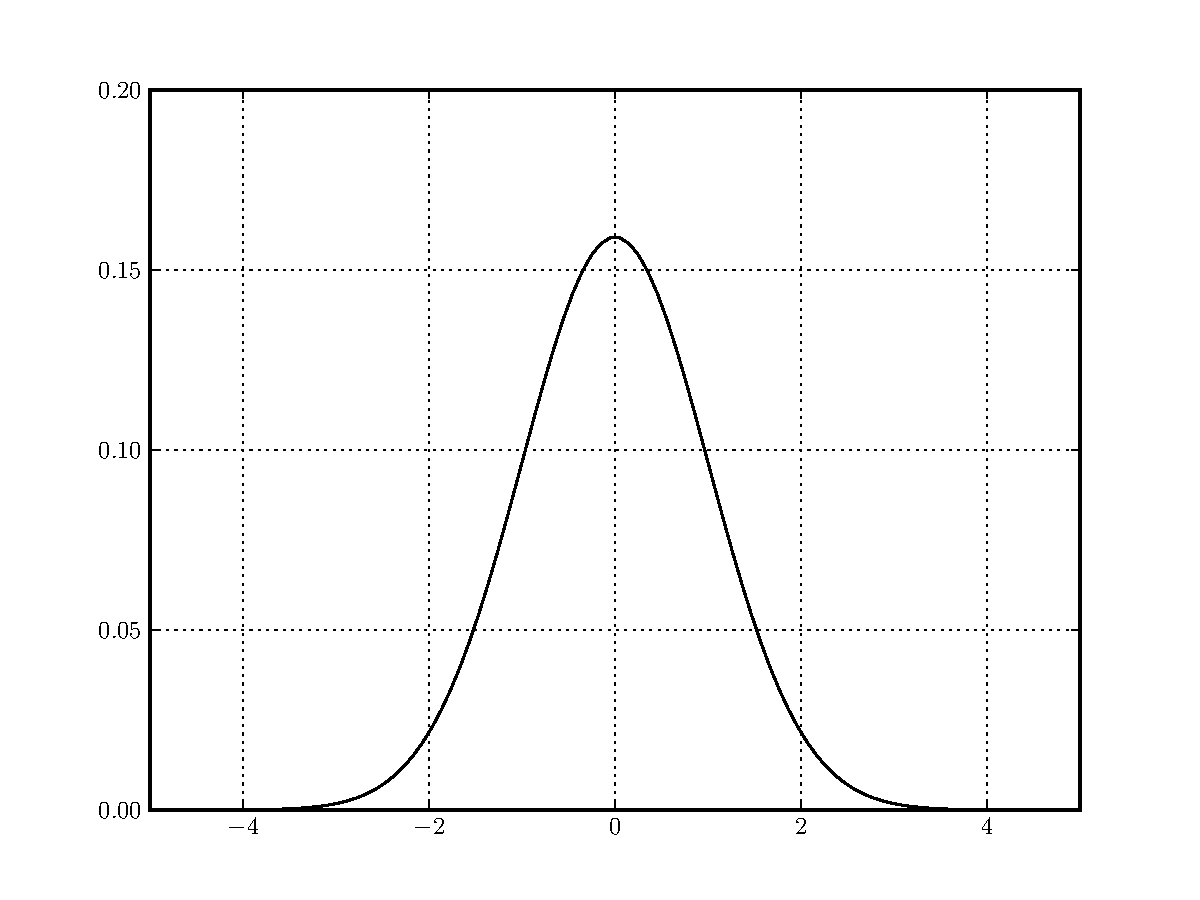
\includegraphics[width=0.7\textwidth]{figures/theory/gaussianKernel.pdf}
	\caption{Vortex blob with Gaussian distribution: [$k=2$,$\sigma=1.0$]}
\end{figure}


\section{Convection of vortex blobs}

The vortex transport equation evaluated using the viscous splitting algorithm. For vortex methods, it is ideal to express the equation \ref{eq:convectionEulerian} in Lagrangian form,

\begin{equation}
\frac{\mathrm{d}\mathbf{x}_p}{\mathrm{d}t} = \mathbf{u}\left(\mathbf{x}_p\right),
\end{equation}
with
\begin{equation}
\frac{\mathrm{d}\omega_p}{\mathrm{d}t} = 0.
\end{equation}

The velocity field can be decomposed using the Helmoltz decomposition,
\begin{equation}
\mathbf{u} = \mathbf{u}_{\infty} + \mathbf{u}_{\omega}
\end{equation}
with \lsymb[t]{$\mathbf{u}_{\infty}$}{Free-stream velocity}{$[m/s]$}{ul} as the free-stream velocity, \lsymb[t]{$\mathbf{u}_{\omega}$}{Vortical velocity}{$[m/s]$}{uxx} as the velocity of the vortical part of the flow.


The velocity can be related to the vorticity using the Biot-Savart law
\begin{equation}
\mathbf{u} = \mathbf{u}_{\infty} + \mathbf{K}\star\omega,
\end{equation}
\begin{equation}
\mathbf{u} = \mathbf{u}_{\infty} + \mathbf{K}\star\omega,
\end{equation}

where the $\star$ represents convolution of the kernel $\mathbf{K}_p$ given by

\begin{equation}
\mathbf{K}_p = \frac{1}{2\pi\left|\mathbf{x}\right|^2}\left(-x_2,x_1\right).
\label{eq:GreensKernel}
\end{equation}

The advantage of discretizing and evaluting the vorticity field in this form is that vortex elements are only needed where the vorticity is nonzero. This means that the vortex elements inherently adapts to domain of interest and does not require simulation of region where nothing happens. From equation \ref{eq:GreensKernel}, we see that it has a singularity when the particles approach each other and so to overcome this we can mollify the kernel using a smooth cutoff function \gsymb[t]{$\zeta$}{Smooth cutoff function}{[-]}{ff}. So the mollified kernel $\mathbf{K}_{\epsilon}$ is given as 

\begin{equation}
\mathbf{K}_{\epsilon} = \mathbf{K} \star \zeta_{\epsilon}.
\end{equation}

	\subsection{Remeshing to treat lagrangian grid distortion}

\section{Diffusion of Vortex Methods}

	\subsection{Modified interpolation kernel}


\section{Boundary conditions at solid boundary}


\section{Simulation acceleration techniques}

\subsection{Fast multi-pole Method}

\subsection{Parallel computation in GPU}




%\section{Convection step}
%
%The convection step of the vorticity transport equation is define by following equation
%
%\begin{equation}
%\frac{d\mathbf{x}_i}{dt} = \mathbf{u}_i\left(\mathbf{x}_1,\mathbf{x}_2,...,\mathbf{x}_N,t\right),
%\end{equation}
%
%and we have to ensure that the circulation is conserved,
%
%\begin{equation}
%\frac{d\Gamma}{dt} = 0.
%\end{equation}

    %
    % Chapter 3: Literature review/Theory of Hybrid vortex methods
   	\chapter{Hybrid Eulerian-Lagrangian Vortex Particle Method}
%\label{ch:LiteratureReview}

% Comparison of hybrid vortex methods.
% choice of hybrid method. Example domain decomposion, coupling technique

%\section{Theory}
%% What is hybrid vortex method?
%% What is the general idea behind the hybrid vortex method?
%% What does it mean to couple particle solver and grid solver?
%% What is the advantage?
%% What is the drawback?
%
%\section{Particle-Grid Coupling techniques}
%% Multiple ways of coupling , VIC, domain decomposition technique
%\subsection{Vortex in Cell method}
%
%\subsection{Particle-Grid domain decomposition methods}
%
%\section{Vortex diffusion methods}
%
%\subsection{Random walk method}
%\subsection{Core expansion method}
%\subsection{Particle-Strength Exchange}
%\subsection{Modified interpolation kernel for diffusion}
%
%\section{Simulation acceleration techniques}
%
%\subsection{Fast multi-pole Method}
%
%\subsection{Parallel computation in GPU}

%\section{Former Work}
%\label{sec:FormerWork}
%
%\subsection{Overview of the Work}
%\label{subsec:OverviewoftheWork}

%\section{Purpose of further research}

%%%%%%%%%%%%%%%%%%%%%%%%%%%%%%%%%%%%%%%%%%%%%%%%%%%%%%%%%%%%%%%%%%%%
%\nomenclature[ak]{$K$}{Kelvin (temperature)}
%\nomenclature[ar]{rpm}{Revolutions per minute (frequency)}
%\nomenclature[ac]{CO}{Carbon Monoxide}
%\nomenclature[ac]{CRM}{Chemical Reaction Modelling}
%\nomenclature[ah]{H2}{Molecular hydrogen}
%\nomenclature[ag]{GSP}{Gas Turbine Simulation Program (Software)}
%\nomenclature[rr]{$\rho$}{Density \nomunit{[$kg/{m^3}$]}}
%\nomenclature[sm]{$\dot{m}$}{Mass flow rate \nomunit{[$kg/s$]}}
%\nomenclature[ab]{bar}{Pressure}

%\nomenclature[rr]{$Re$}{Reynolds number \nomunit{[-]}}
%\nomenclature[rw]{$M$}{Mach number \nomunit{[-]}}
%\nomenclature[rw]{$\mu$}{Dynamic viscosity of air \nomunit{[$kg/{s \cdot m}$]}}
   	%
   	% Chapter 4: Methodology of developing the hybrid vortex method
    %\chapter{Development of the Hybrid Vortex Method for 2D VAWT}
%\label{ch:LiteratureReview}

% Comparison of hybrid vortex methods.
% choice of hybrid method. Example domain decomposion, coupling technique

\section{Methodology}
% What is hybrid vortex method?
% What is the general idea behind the hybrid vortex method?
% What does it mean to couple particle solver and grid solver?
% What is the advantage?
% What is the drawback?

\section{Vortex Method}
% All the info on the development of vortex method
% What approach are you using?
% G. Daenick, G. Winckelmans method

%\documentclass[10pt,a4paper,twocolumn]{article}
%\documentclass[10pt,a4paper]{article}

% Extra packages
%\usepackage{fullpage}
%\usepackage[utf8]{inputenc}
%\usepackage{amsmath}
%\usepackage{amsfonts}
%\usepackage{amssymb}
%\usepackage{graphicx}
%\usepackage{hyperref}

%\usepackage{graphicx}
%\usepackage{caption}
%\usepackage{subcaption}

% Document description
\title{Convergence of modified interpolation kernel for treating diffusion}
\author{Lento Manickathan, 1544101.\\Aerodynamics and Wind energy}

% Begin of main body
%\begin{document}

% Show title
%\maketitle

% Main content

\section{Introduction to modified interpolation kernel for treating diffusion}
The diffusion method that is applied here has been proposed by Shankar and Van Dommelen \cite{Shankar1996} and the modified ${{{\rm{M'}}}_4}$ interpolation kernel has been derived by Ghoniem and Wee \cite{Wee2006} and was also applied by Speck \cite{Speck2011}. The diffusion is simulated by the modified interpolation kernel during the remeshing process. During remeshing, the heat equation is satisfied by transferring the correct fraction of circulation to produce the proper amount of diffusion. The ${{{\rm{M'}}}_4}$ kernel was modified to treat the diffusion and is given by: 

\begin{equation}
{{{\rm{M'}}}_4}\left( {\xi ,c} \right) =
  \begin{cases}
   {1 - \frac{{5{\xi ^2}}}{2} + \frac{{3{{\left| \xi  \right|}^3}}}{2} - {c^2}\left( {2 - 9{\xi ^2} + 6{{\left| \xi  \right|}^3}} \right)} & {\left| \xi \right|} < 1, \\
   \frac{1}{2}{\left( {2 - \left| \xi  \right|} \right)^2}\left( {1 - \left| \xi  \right|} \right) - {c^2}{\left( {2 - \left| \xi  \right|} \right)^2}\left( {1 - 2\left| \xi  \right|} \right) & 1 \le {\left| \xi \right|} < 2,\\
   0 & 2 \le \left| \xi \right|,
  \end{cases}
\label{eq:modInterpKernel}
\end{equation}

where 

\begin{equation}
c = \frac{\sqrt{\nu \Delta t_d}}{\Delta x},
\label{eq:c2}
\end{equation}

and corresponds to the transfer quantity for diffusion. The $\nu$ denotes the viscosity of the fluid, $t_d$ is the diffusion time step and $\Delta x$ is the blob spacing. When $c \rightarrow 0$, the interpolation kernel turns to the classical non-diffusion kernel.  This modified interpolation kernel conserves the circulation of each vortex and also satisfies the conservation of linear and angular momentum of the vorticies.\\

The vortex method employs the viscous splitting procedure, where the vortex blobs are convected first and is then diffused through the remeshing process using the modified interpolation kernel. The advantage of this methodology is that the convection process is not constrained by the CFL condition. So, the convection time step size can be different than from the diffusion time step size and the diffusion time step size is a multiple of the convection time step size depending on the redistribution frequency $f_{redist}$. Therefore, the constrained that is imposed on the redistribution frequency is the stability bounds of the modified interpolation kernel. Analyzing the amplification factor and the phase error of the modified interpolation kernel in the Fourier space requires that the $c^2$ should be as follows:


\begin{equation}
\frac{1}{6} \le c^2 \le \frac{1}{2}.
\label{eq:c2stability}
\end{equation}

This will ensure the stability of the problem and will suppress any spurious oscillations and ensure that it is a non-negative interpolation kernel with non-negative redistribution fractions.

\section{Errors in Blob Initialization}
To verify the accuracy of the diffusion process, the error of the discrete solution was compared against the analytical solution of the Lamb-Oseen vortex where the vorticity field

\begin{equation}
\omega\left(x,t\right) = \frac{\Gamma_o}{4\pi \nu t} \exp \left(-\frac{r^2}{4 \nu t} \right),
\label{eq:LambOseen}
\end{equation}

was used as the analytical solution for a given viscosity $\nu$ at a given time $t$ with a unit circulation $\Gamma_o$. In order to quantify the error generated during discretization, the discrete $L^2$-norm error was calculated as 

\begin{equation}
{\left\| {{\omega ^{{\rm{exact}}}} - {\omega ^{{\rm{discrete}}}}} \right\|_2} = {\left( {\sum\limits_i {{{\left| {{\omega ^{{\rm{exact}}}}({{\bf{x}}_i}) - {\omega ^{{\rm{discrete}}}}({{\bf{x}}_i})} \right|}^2}\Delta x\Delta y} } \right)^{\frac{1}{2}}},
\label{eq:L2normEq}
\end{equation} 	

and the discrete maximum relative error in vorticity was evaluated as follows:

\begin{equation}
{\left\| {{\omega ^{{\rm{exact}}}} - {\omega ^{{\rm{discrete}}}}} \right\|_\infty } = \frac{{\max \left\{ {\left| {{\omega ^{{\rm{exact}}}}({{\bf{x}}_i}) - {\omega ^{{\rm{discrete}}}}({{\bf{x}}_i})} \right|:i \in {\mathcal{S}}} \right\}}}{{\max \left\{ {\left| {{\omega ^{{\rm{exact}}}}({{\bf{x}}_i})} \right|:i \in {\mathcal{S}}} \right\}}}.
\label{eq:maxRelEq}
\end{equation}

During the initial discretization, it was seen that in order to obtain the correct vorticity field, you need to take in account of the numerical diffusion. As Barba had shown in \cite{Barba2004a}, in order to properly account for the diffusion effect when discretization with gaussian blobs (with $k=2$), a time-shift correction equivalent to shifting the initial time by $\sigma^2/2\nu$ needs to be applied. This follows directly from the discretization of the general solution of the heat equation with these gaussian cores. With this proper time-shifting, you can ensure the accurate initialization of the Lamb-Oseen vortex for the error evaluations. \\

An alternate method of taking account for the gaussian approximation is the Beale's iterative method for circulation processing. The concept is based on iteratively improving the circulation values of the gaussian blobs so that it gives a better approximation of the local vorticity that the blobs are trying to represent. The downside to this processing is that the influence matrix for the calculation is $\mathcal{O}(N^2)$ and requires large computational resources.

\section{Importance of initial conditions}



\begin{itemize}
\item Comparing $\nu=0.01$ and $\nu=0.0005$ with various starting times. Show the growth in error. 
\item Compare various correction methods for initial discretization. Beale vs. time-shifting
\end{itemize}

\section{Convergence of the vortex method with diffusion}
The discretization errors of the vortex method was evaluated to check for the convergence of its error to the exact solution. If the modified interpolation kernel was accurately implemented into the vortex method, the spatial and the temporal discretization error of the vortex method should converge as you refine the parameters. When checking for discretization error a given parameter, all the other parameters was kept constant and at a very high resolution. This ensured that the significant error emerges from the discretization of the chosen parameter. For the initial investigations, this meant that the $c^2$ parameter of the kernel diffusion term was also varying dependent on the discretization parameter. This could indirect influence on the convergence rate, as diffusion term was varying for each discrete value. So, a second investigation was done, where the $c^2$ parameters was kept constant by varying the appropriate values.

To ensure that other numerical error does not dominate and the consistency of the simulations, all the variables were carefully chosen and are tabulated in table \ref{tab:refinementParameters}.\\

\begin{table}[hbt]
\centering
	\begin{tabular}{|l|r|}
	\hline \textbf{Parameters} 					& \textbf{Value} \\
	\hline Domain $\Omega$ 						& $[-2, 2]^2$ \\
	Overlap ratio $\Delta h/\sigma$  	& 0.5  \\ 
	Viscous time scale $\tau$ 			& 0.0200 to 0.0250 \\
	Time step scheme 					& RK4 \\
	Vortex viscosity $\nu$ 				& [0.01, 0.0005] \\
	Vortex Circulation Strength $\Gamma$ & $2 \pi$ \\
	Vortex Reynolds Number Re 			& [50, 2000] \\
	Vortex Reynolds Number Re 			& [50, 2000] \\
	Kernel diffusion parameter $c^2$		& $1/6$, $1/4$, $1/2$ \\
	Redistribution frequency $f_{redist}$& 1 \\
	Population control $\Gamma_{min}$ 	& \texttt{eps} $ = 2.2e$\textrm{-}$16$\\
	Population control frequency $f_{pc}$& 1 \\
	\hline 
	\end{tabular} 
\caption{Refinement study parameters}
\label{tab:refinementParameters}
\end{table}


\subsection{Blob density refinement study}
In order to investigate the convergence of the error and as the spatial discretization is refined, a blob density refinement study was undertaken. By increasing the number of blob cores to represent the given vortex, the discrete approximation of the vortex should converge to the exact solution. In order words, as the spatial discretization $\Delta y$ and $\Delta y$ is reduced, the error should converge.

During the investigation of the blob density (number of particles) refinement, the time step was maintained at a minimum to reduce its error, $\delta T = 0.05$. Investigation was done for two viscous cases, as shown in table \ref{tab:refinementParameters}. This results in time step parameters as shown in table \ref{tab:spatialRefinementParameters}.

\begin{table}[hbt]
\centering
	\begin{tabular}{|l|r|r|}
	\hline \textbf{Parameters} 	& \textbf{$\nu = 0.01$} & \textbf{$\nu = 0.0005$}\\
	\hline Start time $\tau/\nu$    & 2 & 40 \\				
	Stop time  $\tau/\nu$ 	& 2.5 & 50 \\
	Number of steps 			& 10 & 200 \\
	Number of blobs 			& [73, 86, 98, 108, 118, 126] & [327, 386, 438, 484, 527, 566]\\
	\hline
	\end{tabular}
\caption{Blob density refinement study parameters}
\label{tab:spatialRefinementParameters}	
\end{table}

The results of the spatial refinement is shown in figure \ref{fig:wErrorVSdx_varyingC2}. 

\begin{figure}[!tbhp]
\centering
	\begin{subfigure}{0.48\textwidth}
		\centering
		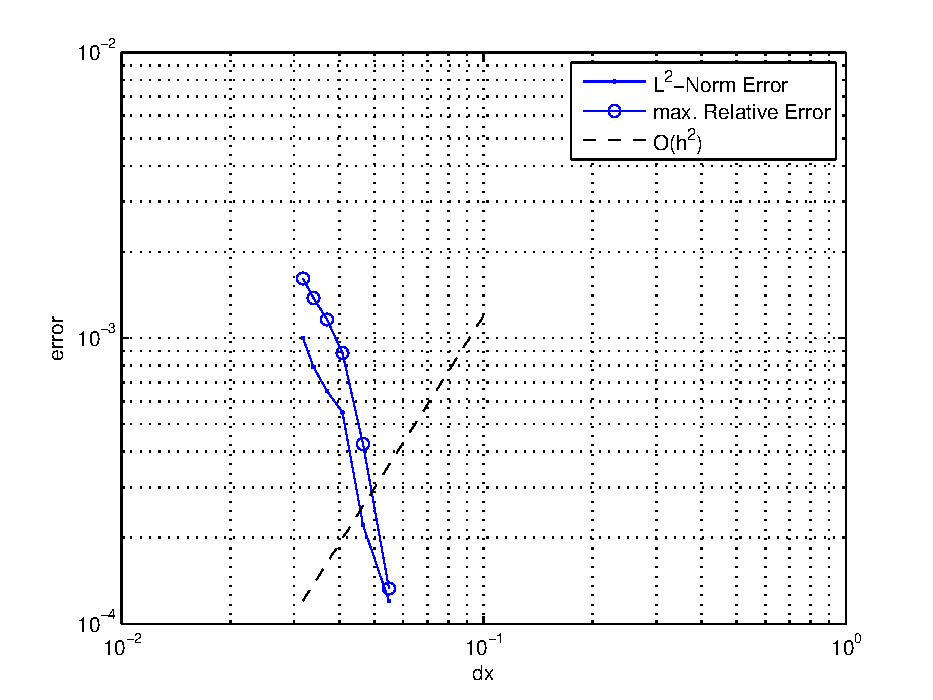
\includegraphics[width=\textwidth]{./figures/wErrorVSdx_nu001_c2vary.pdf}	
		\caption{$\nu=0.01$}
	\end{subfigure}
	\begin{subfigure}{0.48\textwidth}
		\centering
		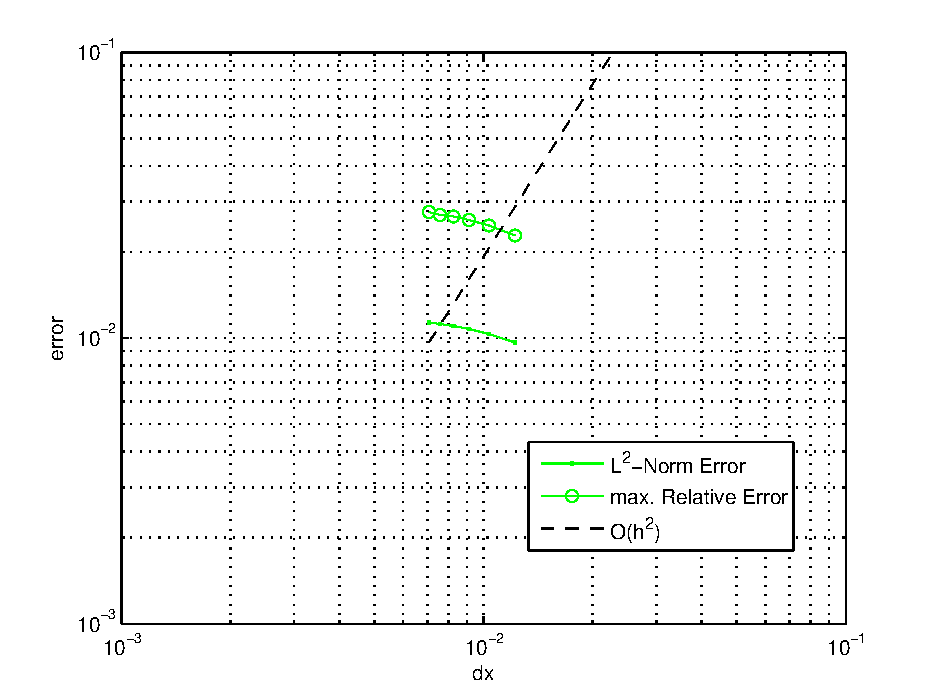
\includegraphics[width=\textwidth]{./figures/wErrorVSdx_nu00005_c2vary.pdf}	
		\caption{$\nu=0.0005$}
	\end{subfigure}
\caption{Spatial refinement with a varying $c^2$}
\label{fig:wErrorVSdx_varyingC2}
\end{figure}

It is evident that the order of convergence does not match the predicted one. This is because of the one key parameter, the kernel diffusion parameter $c^2$. We assume that as the number of particles (i.e blob density) increases, the spatial discretization $\Delta h$ reduces thereby resolving the Lamb-Oseen vortex to greater detail. However, from equation \ref{eq:c2} we see that if viscosity $nu$ and time step $\Delta T$ is constant then $\Delta $ is inverse proportional to kernel diffusion parameter $c^2$. This means that the $c^2$ parameter is increasing and has a direct influence of the damping of the numerical oscillations. Therefore, as the $c^2$ increase, the growth in error might be more dominant and could have an effect on the spatial refinement study.\\

So, to have a proper comparison, the spatial refinement study was done with keeping the $c^2$ parameter constant, figure \ref{fig:wErrorVSdx_constantC2}.

\begin{figure}[!tbhp]
\centering
	\begin{subfigure}{0.48\textwidth}
		\centering
		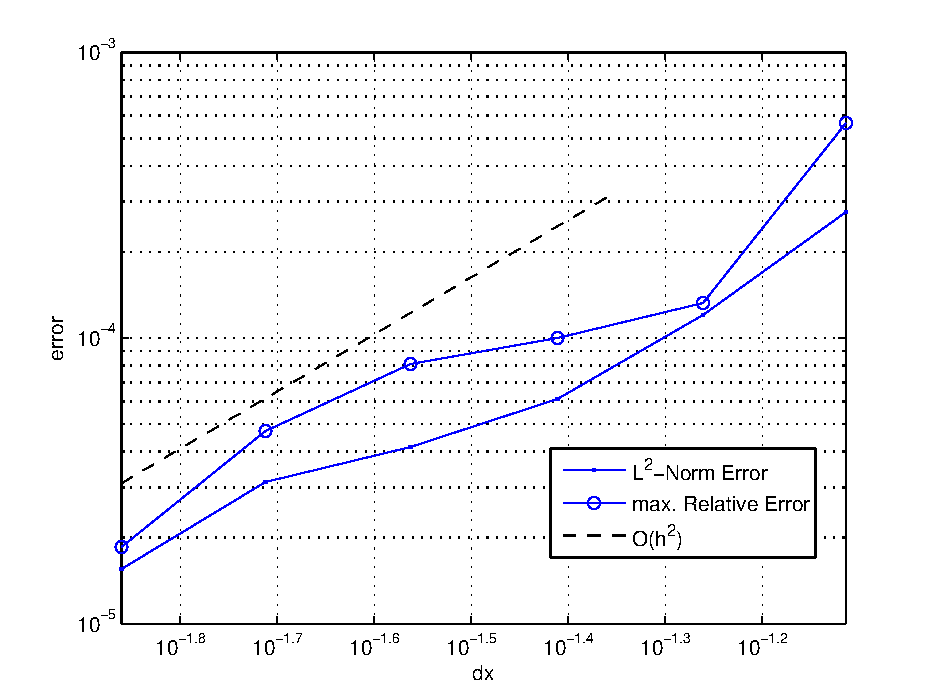
\includegraphics[width=\textwidth]{./figures/wErrorVSdx_nu0p01_constantc2.pdf}	
		\caption{$\nu=0.01$}
	\end{subfigure}
	\begin{subfigure}{0.48\textwidth}
		\centering
		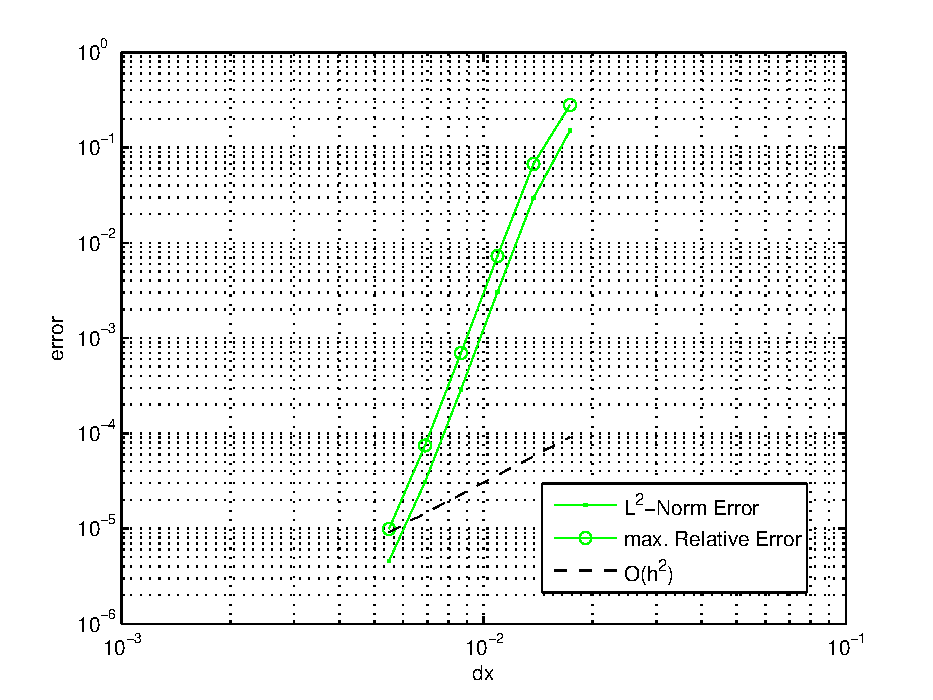
\includegraphics[width=\textwidth]{./figures/wErrorVSdx_nu0p0005_constantc2.pdf}	
		\caption{$\nu=0.0005$}
	\end{subfigure}
\caption{Spatial refinement with a constant $c^2=1/6$}
\label{fig:wErrorVSdx_constantC2}
\end{figure}

Now we can see that the error converges as you reduced the blob mesh size. This is the correct trend that we are looking for.

\subsection{Spatial refinement for various kernel diffusion parameter}

\begin{figure}[!tbhp]
\centering
	\begin{subfigure}{0.48\textwidth}
		\centering
		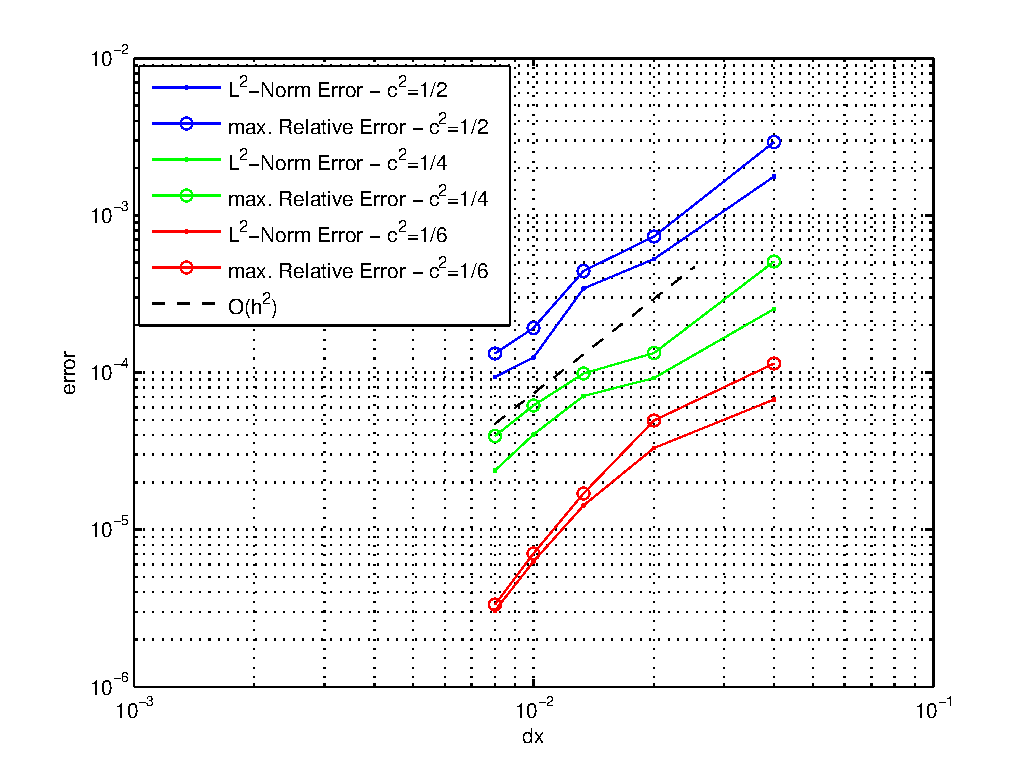
\includegraphics[width=\textwidth]{./figures/wErrorVSdx_nu0p01_variousC2.pdf}	
		\caption{$\nu=0.01$}
	\end{subfigure}
	\begin{subfigure}{0.48\textwidth}
		\centering
		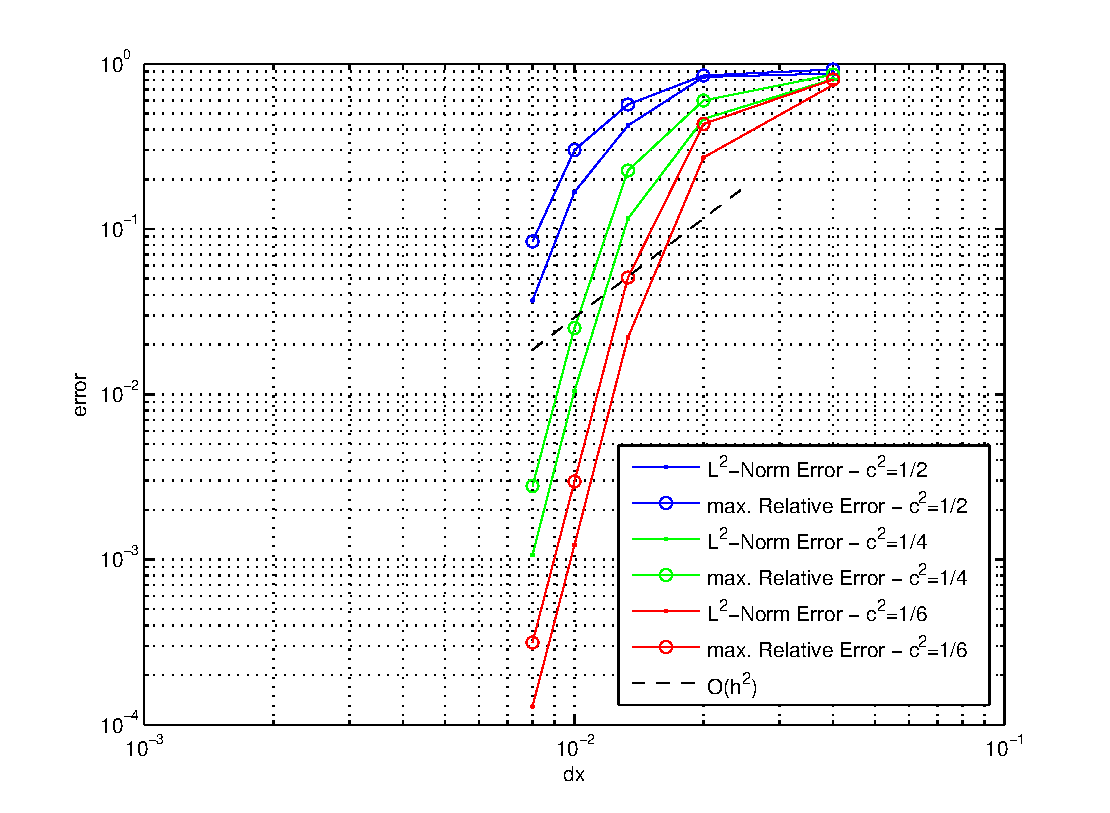
\includegraphics[width=\textwidth]{./figures/wErrorVSdx_nu0p0005_variousC2.pdf}	
		\caption{$\nu=0.0005$}
	\end{subfigure}
\caption{Spatial refinment for various $c^2$ parameters, $c^2 = [\frac{1}{6}, \frac{1}{4}, \frac{1}{2}]$}
\label{fig:wErrorVSdx_variousC2}
\end{figure}



\subsection{Time Step refinement study}

\begin{figure}[!tbhp]
\centering
	\begin{subfigure}{0.48\textwidth}
		\centering
		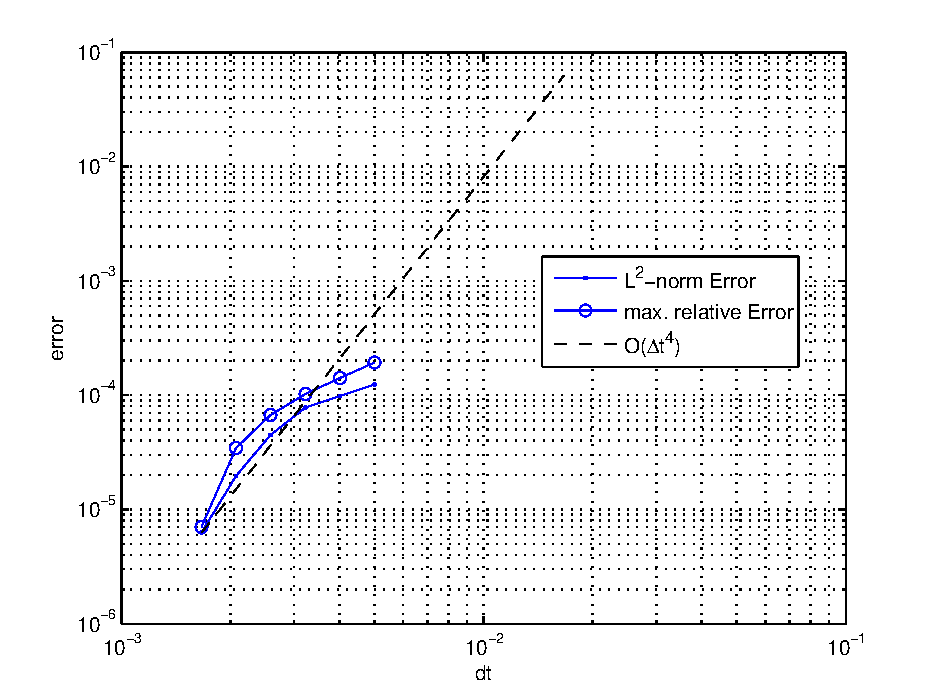
\includegraphics[width=\textwidth]{./figures/wErrorVSdt_nu0p01_varyingC2.pdf}	
		\caption{$\nu=0.01$}
	\end{subfigure}
	\begin{subfigure}{0.48\textwidth}
		\centering
		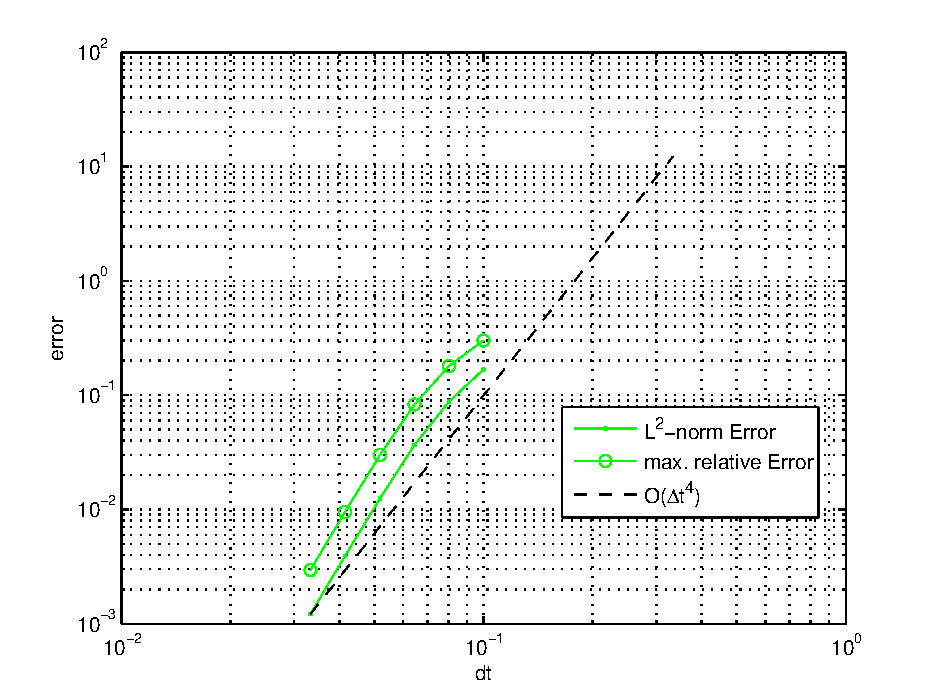
\includegraphics[width=\textwidth]{./figures/wErrorVSdt_nu0p0005_varyingC2.pdf}	
		\caption{$\nu=0.0005$}
	\end{subfigure}
\caption{Time Step refinement with a varying $c^2$}
\label{fig:wErrorVSdt_varyingC2}
\end{figure}





% End of main body
\newpage

% Bibliography
%\bibliographystyle{plain}
%\bibliography{../../Literature/library}

% End of document
%\end{document}

\subsection{Blob Discretization}
% Particle initialization
% info on cut-off function
% what are the governing variables? Overlap ratio, grid size, 

\subsubsection{Error analysis of discretization}
% importance of time-shift correction when comparing with Lamb-oseen
% overlap ratio vs. L2-norm and max.relative error
% number of particles/ deltaH vs. L2-norm and max.relative error

\subsection{Vortex blob convection}
% Info on time-stepping scheme
% source of error during convection = lagrangian distortion from fluid strain
% importance of population control

\subsubsection{Remeshing for lagrangian grid distortion}
% show with and without remeshing figure.
% investigate on remeshing frequence -> treatment of vortex diffusion

\subsubsection{Error of time-Stepping}
% Time-step vs. L2-norm and max.relative error
% Show the convergence of time-step scheme

\subsection{Treatment of vortex diffusion with remeshing}
% refer to Daehyun Wee, Ahmed F. Ghoniem 2006
% Brief overview of other methods
% motivation of the choice of modified interpolation kernel, diffusion through remeshing


\subsubsection{Modified interpolation kernel}
% Equation for modified interpolation kernel, 
% M4 kernel
% Stability condition, And also conclusion to c2 parameter. the range for the value 1/6<= c2 <=1/2

\subsubsection{Convergence of modified interpolation kernel}
% Comparison with L.Barba, Phd.Thesis
% evolution of error in vorticity of Lamb-oseen.
% 

%%%%%%%%
\subsection{Treatment of geometry in fluid}

\subsubsection{Vortex sheet for inviscid boundary condition}
% using vortex sheet to solve boundary integral equation
% refer to using RBF kernels as a mesh-less solution, recommendations.

\subsubsection{Convergence of panel method}


%%%%%%%
\section{Coupling grid to particle solver}

\subsection{Coupling algorithm and modified overlap region}


\section{Moving boundaries}
\subsection{Modification to grid solver}
\subsection{Modification to vortex method}


%\section{Former Work}
%\label{sec:FormerWork}
%
%\subsection{Overview of the Work}
%\label{subsec:OverviewoftheWork}

%\section{Purpose of further research}

%%%%%%%%%%%%%%%%%%%%%%%%%%%%%%%%%%%%%%%%%%%%%%%%%%%%%%%%%%%%%%%%%%%%
%\nomenclature[ak]{$K$}{Kelvin (temperature)}
%\nomenclature[ar]{rpm}{Revolutions per minute (frequency)}
%\nomenclature[ac]{CO}{Carbon Monoxide}
%\nomenclature[ac]{CRM}{Chemical Reaction Modelling}
%\nomenclature[ah]{H2}{Molecular hydrogen}
%\nomenclature[ag]{GSP}{Gas Turbine Simulation Program (Software)}
%\nomenclature[rr]{$\rho$}{Density \nomunit{[$kg/{m^3}$]}}
%\nomenclature[sm]{$\dot{m}$}{Mass flow rate \nomunit{[$kg/s$]}}
%\nomenclature[ab]{bar}{Pressure}

%\nomenclature[rr]{$Re$}{Reynolds number \nomunit{[-]}}
%\nomenclature[rw]{$M$}{Mach number \nomunit{[-]}}
%\nomenclature[rw]{$\mu$}{Dynamic viscosity of air \nomunit{[$kg/{s \cdot m}$]}}
    %%\documentclass[10pt,a4paper,twocolumn]{article}
%\documentclass[10pt,a4paper]{article}

% Extra packages
%\usepackage{fullpage}
%\usepackage[utf8]{inputenc}
%\usepackage{amsmath}
%\usepackage{amsfonts}
%\usepackage{amssymb}
%\usepackage{graphicx}
%\usepackage{hyperref}

%\usepackage{graphicx}
%\usepackage{caption}
%\usepackage{subcaption}

% Document description
\title{Convergence of modified interpolation kernel for treating diffusion}
\author{Lento Manickathan, 1544101.\\Aerodynamics and Wind energy}

% Begin of main body
%\begin{document}

% Show title
%\maketitle

% Main content

\section{Introduction to modified interpolation kernel for treating diffusion}
The diffusion method that is applied here has been proposed by Shankar and Van Dommelen \cite{Shankar1996} and the modified ${{{\rm{M'}}}_4}$ interpolation kernel has been derived by Ghoniem and Wee \cite{Wee2006} and was also applied by Speck \cite{Speck2011}. The diffusion is simulated by the modified interpolation kernel during the remeshing process. During remeshing, the heat equation is satisfied by transferring the correct fraction of circulation to produce the proper amount of diffusion. The ${{{\rm{M'}}}_4}$ kernel was modified to treat the diffusion and is given by: 

\begin{equation}
{{{\rm{M'}}}_4}\left( {\xi ,c} \right) =
  \begin{cases}
   {1 - \frac{{5{\xi ^2}}}{2} + \frac{{3{{\left| \xi  \right|}^3}}}{2} - {c^2}\left( {2 - 9{\xi ^2} + 6{{\left| \xi  \right|}^3}} \right)} & {\left| \xi \right|} < 1, \\
   \frac{1}{2}{\left( {2 - \left| \xi  \right|} \right)^2}\left( {1 - \left| \xi  \right|} \right) - {c^2}{\left( {2 - \left| \xi  \right|} \right)^2}\left( {1 - 2\left| \xi  \right|} \right) & 1 \le {\left| \xi \right|} < 2,\\
   0 & 2 \le \left| \xi \right|,
  \end{cases}
\label{eq:modInterpKernel}
\end{equation}

where 

\begin{equation}
c = \frac{\sqrt{\nu \Delta t_d}}{\Delta x},
\label{eq:c2}
\end{equation}

and corresponds to the transfer quantity for diffusion. The $\nu$ denotes the viscosity of the fluid, $t_d$ is the diffusion time step and $\Delta x$ is the blob spacing. When $c \rightarrow 0$, the interpolation kernel turns to the classical non-diffusion kernel.  This modified interpolation kernel conserves the circulation of each vortex and also satisfies the conservation of linear and angular momentum of the vorticies.\\

The vortex method employs the viscous splitting procedure, where the vortex blobs are convected first and is then diffused through the remeshing process using the modified interpolation kernel. The advantage of this methodology is that the convection process is not constrained by the CFL condition. So, the convection time step size can be different than from the diffusion time step size and the diffusion time step size is a multiple of the convection time step size depending on the redistribution frequency $f_{redist}$. Therefore, the constrained that is imposed on the redistribution frequency is the stability bounds of the modified interpolation kernel. Analyzing the amplification factor and the phase error of the modified interpolation kernel in the Fourier space requires that the $c^2$ should be as follows:


\begin{equation}
\frac{1}{6} \le c^2 \le \frac{1}{2}.
\label{eq:c2stability}
\end{equation}

This will ensure the stability of the problem and will suppress any spurious oscillations and ensure that it is a non-negative interpolation kernel with non-negative redistribution fractions.

\section{Errors in Blob Initialization}
To verify the accuracy of the diffusion process, the error of the discrete solution was compared against the analytical solution of the Lamb-Oseen vortex where the vorticity field

\begin{equation}
\omega\left(x,t\right) = \frac{\Gamma_o}{4\pi \nu t} \exp \left(-\frac{r^2}{4 \nu t} \right),
\label{eq:LambOseen}
\end{equation}

was used as the analytical solution for a given viscosity $\nu$ at a given time $t$ with a unit circulation $\Gamma_o$. In order to quantify the error generated during discretization, the discrete $L^2$-norm error was calculated as 

\begin{equation}
{\left\| {{\omega ^{{\rm{exact}}}} - {\omega ^{{\rm{discrete}}}}} \right\|_2} = {\left( {\sum\limits_i {{{\left| {{\omega ^{{\rm{exact}}}}({{\bf{x}}_i}) - {\omega ^{{\rm{discrete}}}}({{\bf{x}}_i})} \right|}^2}\Delta x\Delta y} } \right)^{\frac{1}{2}}},
\label{eq:L2normEq}
\end{equation} 	

and the discrete maximum relative error in vorticity was evaluated as follows:

\begin{equation}
{\left\| {{\omega ^{{\rm{exact}}}} - {\omega ^{{\rm{discrete}}}}} \right\|_\infty } = \frac{{\max \left\{ {\left| {{\omega ^{{\rm{exact}}}}({{\bf{x}}_i}) - {\omega ^{{\rm{discrete}}}}({{\bf{x}}_i})} \right|:i \in {\mathcal{S}}} \right\}}}{{\max \left\{ {\left| {{\omega ^{{\rm{exact}}}}({{\bf{x}}_i})} \right|:i \in {\mathcal{S}}} \right\}}}.
\label{eq:maxRelEq}
\end{equation}

During the initial discretization, it was seen that in order to obtain the correct vorticity field, you need to take in account of the numerical diffusion. As Barba had shown in \cite{Barba2004a}, in order to properly account for the diffusion effect when discretization with gaussian blobs (with $k=2$), a time-shift correction equivalent to shifting the initial time by $\sigma^2/2\nu$ needs to be applied. This follows directly from the discretization of the general solution of the heat equation with these gaussian cores. With this proper time-shifting, you can ensure the accurate initialization of the Lamb-Oseen vortex for the error evaluations. \\

An alternate method of taking account for the gaussian approximation is the Beale's iterative method for circulation processing. The concept is based on iteratively improving the circulation values of the gaussian blobs so that it gives a better approximation of the local vorticity that the blobs are trying to represent. The downside to this processing is that the influence matrix for the calculation is $\mathcal{O}(N^2)$ and requires large computational resources.

\section{Importance of initial conditions}



\begin{itemize}
\item Comparing $\nu=0.01$ and $\nu=0.0005$ with various starting times. Show the growth in error. 
\item Compare various correction methods for initial discretization. Beale vs. time-shifting
\end{itemize}

\section{Convergence of the vortex method with diffusion}
The discretization errors of the vortex method was evaluated to check for the convergence of its error to the exact solution. If the modified interpolation kernel was accurately implemented into the vortex method, the spatial and the temporal discretization error of the vortex method should converge as you refine the parameters. When checking for discretization error a given parameter, all the other parameters was kept constant and at a very high resolution. This ensured that the significant error emerges from the discretization of the chosen parameter. For the initial investigations, this meant that the $c^2$ parameter of the kernel diffusion term was also varying dependent on the discretization parameter. This could indirect influence on the convergence rate, as diffusion term was varying for each discrete value. So, a second investigation was done, where the $c^2$ parameters was kept constant by varying the appropriate values.

To ensure that other numerical error does not dominate and the consistency of the simulations, all the variables were carefully chosen and are tabulated in table \ref{tab:refinementParameters}.\\

\begin{table}[hbt]
\centering
	\begin{tabular}{|l|r|}
	\hline \textbf{Parameters} 					& \textbf{Value} \\
	\hline Domain $\Omega$ 						& $[-2, 2]^2$ \\
	Overlap ratio $\Delta h/\sigma$  	& 0.5  \\ 
	Viscous time scale $\tau$ 			& 0.0200 to 0.0250 \\
	Time step scheme 					& RK4 \\
	Vortex viscosity $\nu$ 				& [0.01, 0.0005] \\
	Vortex Circulation Strength $\Gamma$ & $2 \pi$ \\
	Vortex Reynolds Number Re 			& [50, 2000] \\
	Vortex Reynolds Number Re 			& [50, 2000] \\
	Kernel diffusion parameter $c^2$		& $1/6$, $1/4$, $1/2$ \\
	Redistribution frequency $f_{redist}$& 1 \\
	Population control $\Gamma_{min}$ 	& \texttt{eps} $ = 2.2e$\textrm{-}$16$\\
	Population control frequency $f_{pc}$& 1 \\
	\hline 
	\end{tabular} 
\caption{Refinement study parameters}
\label{tab:refinementParameters}
\end{table}


\subsection{Blob density refinement study}
In order to investigate the convergence of the error and as the spatial discretization is refined, a blob density refinement study was undertaken. By increasing the number of blob cores to represent the given vortex, the discrete approximation of the vortex should converge to the exact solution. In order words, as the spatial discretization $\Delta y$ and $\Delta y$ is reduced, the error should converge.

During the investigation of the blob density (number of particles) refinement, the time step was maintained at a minimum to reduce its error, $\delta T = 0.05$. Investigation was done for two viscous cases, as shown in table \ref{tab:refinementParameters}. This results in time step parameters as shown in table \ref{tab:spatialRefinementParameters}.

\begin{table}[hbt]
\centering
	\begin{tabular}{|l|r|r|}
	\hline \textbf{Parameters} 	& \textbf{$\nu = 0.01$} & \textbf{$\nu = 0.0005$}\\
	\hline Start time $\tau/\nu$    & 2 & 40 \\				
	Stop time  $\tau/\nu$ 	& 2.5 & 50 \\
	Number of steps 			& 10 & 200 \\
	Number of blobs 			& [73, 86, 98, 108, 118, 126] & [327, 386, 438, 484, 527, 566]\\
	\hline
	\end{tabular}
\caption{Blob density refinement study parameters}
\label{tab:spatialRefinementParameters}	
\end{table}

The results of the spatial refinement is shown in figure \ref{fig:wErrorVSdx_varyingC2}. 

\begin{figure}[!tbhp]
\centering
	\begin{subfigure}{0.48\textwidth}
		\centering
		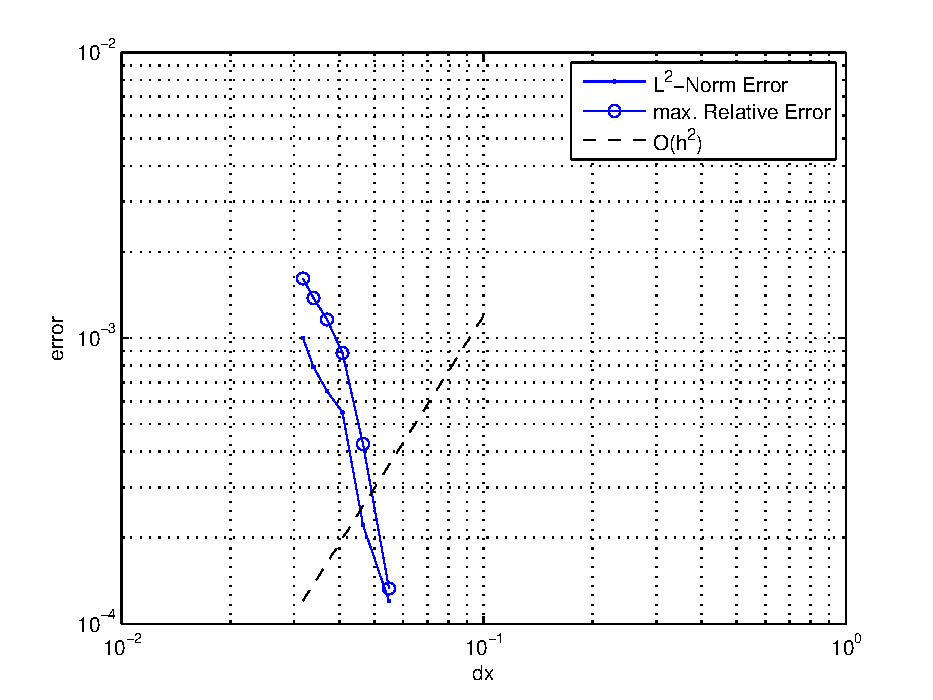
\includegraphics[width=\textwidth]{./figures/wErrorVSdx_nu001_c2vary.pdf}	
		\caption{$\nu=0.01$}
	\end{subfigure}
	\begin{subfigure}{0.48\textwidth}
		\centering
		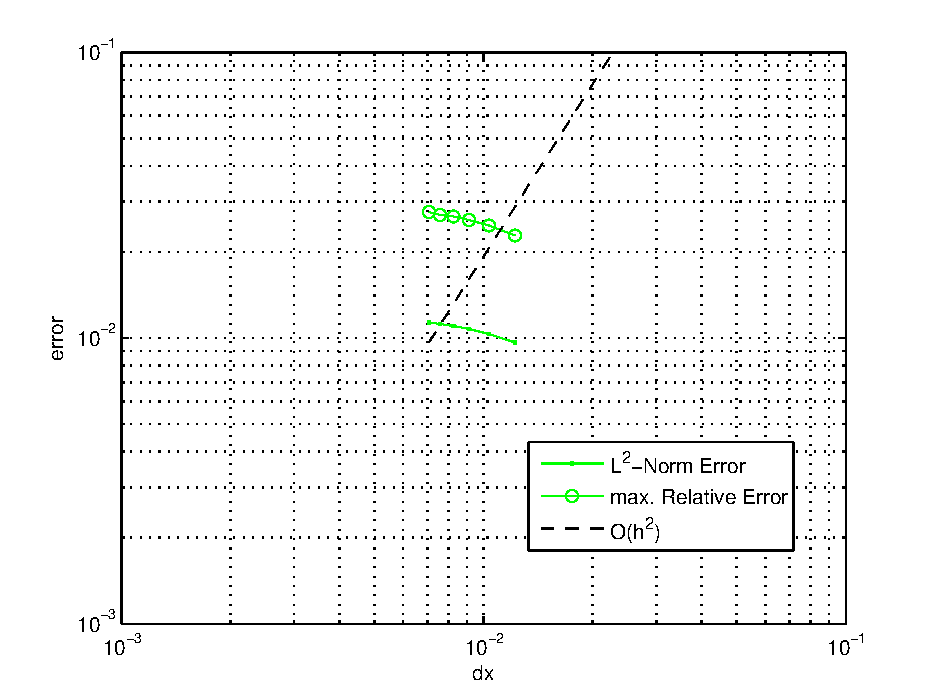
\includegraphics[width=\textwidth]{./figures/wErrorVSdx_nu00005_c2vary.pdf}	
		\caption{$\nu=0.0005$}
	\end{subfigure}
\caption{Spatial refinement with a varying $c^2$}
\label{fig:wErrorVSdx_varyingC2}
\end{figure}

It is evident that the order of convergence does not match the predicted one. This is because of the one key parameter, the kernel diffusion parameter $c^2$. We assume that as the number of particles (i.e blob density) increases, the spatial discretization $\Delta h$ reduces thereby resolving the Lamb-Oseen vortex to greater detail. However, from equation \ref{eq:c2} we see that if viscosity $nu$ and time step $\Delta T$ is constant then $\Delta $ is inverse proportional to kernel diffusion parameter $c^2$. This means that the $c^2$ parameter is increasing and has a direct influence of the damping of the numerical oscillations. Therefore, as the $c^2$ increase, the growth in error might be more dominant and could have an effect on the spatial refinement study.\\

So, to have a proper comparison, the spatial refinement study was done with keeping the $c^2$ parameter constant, figure \ref{fig:wErrorVSdx_constantC2}.

\begin{figure}[!tbhp]
\centering
	\begin{subfigure}{0.48\textwidth}
		\centering
		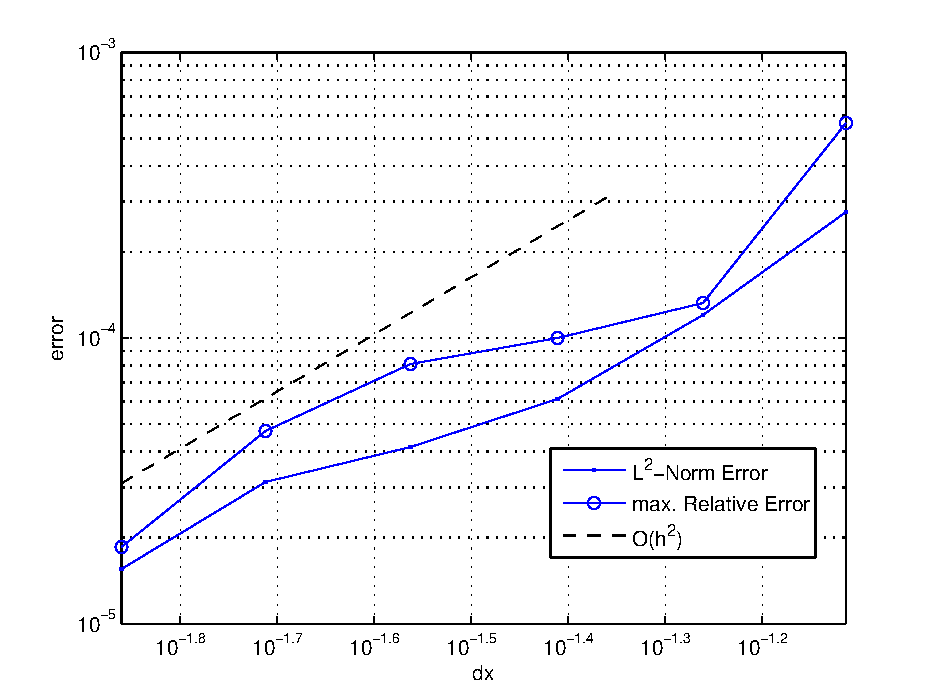
\includegraphics[width=\textwidth]{./figures/wErrorVSdx_nu0p01_constantc2.pdf}	
		\caption{$\nu=0.01$}
	\end{subfigure}
	\begin{subfigure}{0.48\textwidth}
		\centering
		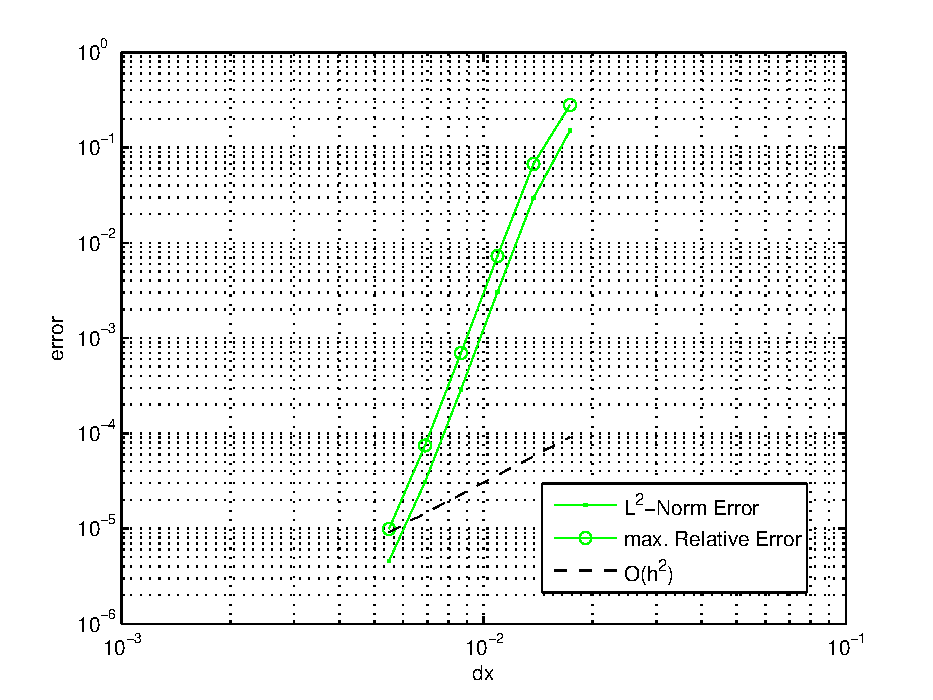
\includegraphics[width=\textwidth]{./figures/wErrorVSdx_nu0p0005_constantc2.pdf}	
		\caption{$\nu=0.0005$}
	\end{subfigure}
\caption{Spatial refinement with a constant $c^2=1/6$}
\label{fig:wErrorVSdx_constantC2}
\end{figure}

Now we can see that the error converges as you reduced the blob mesh size. This is the correct trend that we are looking for.

\subsection{Spatial refinement for various kernel diffusion parameter}

\begin{figure}[!tbhp]
\centering
	\begin{subfigure}{0.48\textwidth}
		\centering
		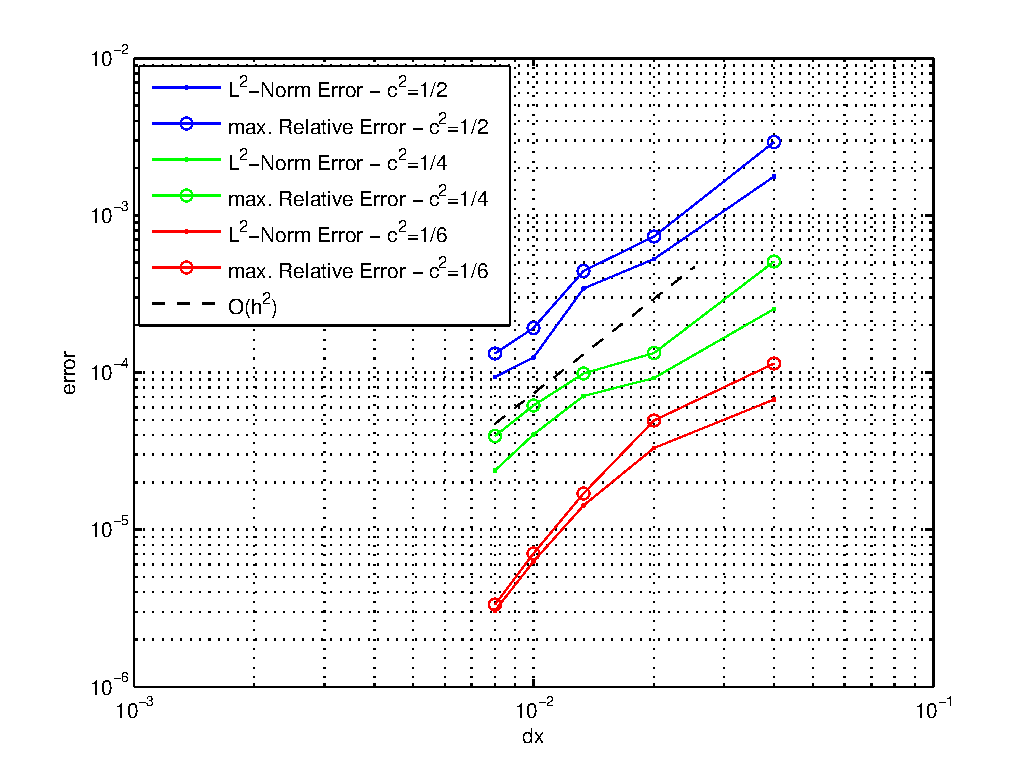
\includegraphics[width=\textwidth]{./figures/wErrorVSdx_nu0p01_variousC2.pdf}	
		\caption{$\nu=0.01$}
	\end{subfigure}
	\begin{subfigure}{0.48\textwidth}
		\centering
		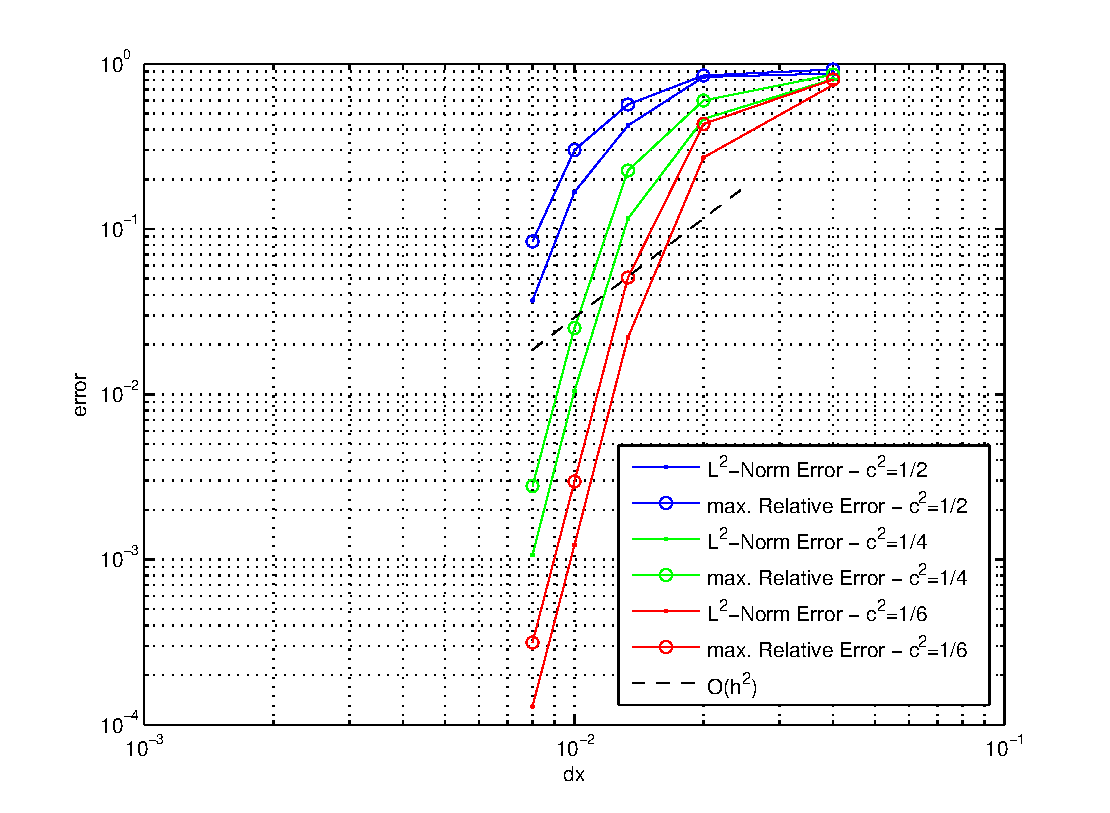
\includegraphics[width=\textwidth]{./figures/wErrorVSdx_nu0p0005_variousC2.pdf}	
		\caption{$\nu=0.0005$}
	\end{subfigure}
\caption{Spatial refinment for various $c^2$ parameters, $c^2 = [\frac{1}{6}, \frac{1}{4}, \frac{1}{2}]$}
\label{fig:wErrorVSdx_variousC2}
\end{figure}



\subsection{Time Step refinement study}

\begin{figure}[!tbhp]
\centering
	\begin{subfigure}{0.48\textwidth}
		\centering
		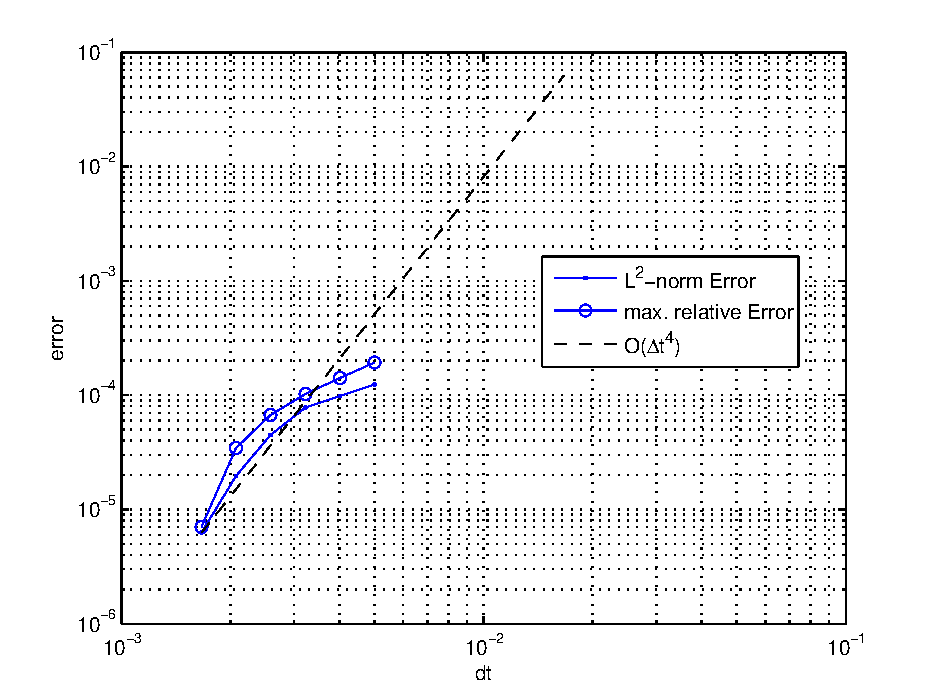
\includegraphics[width=\textwidth]{./figures/wErrorVSdt_nu0p01_varyingC2.pdf}	
		\caption{$\nu=0.01$}
	\end{subfigure}
	\begin{subfigure}{0.48\textwidth}
		\centering
		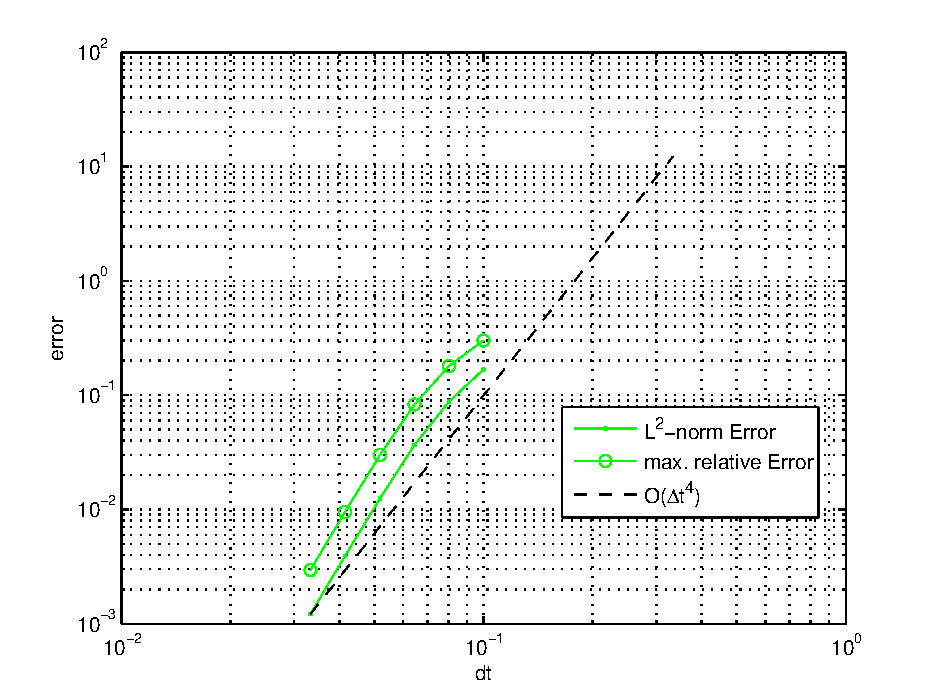
\includegraphics[width=\textwidth]{./figures/wErrorVSdt_nu0p0005_varyingC2.pdf}	
		\caption{$\nu=0.0005$}
	\end{subfigure}
\caption{Time Step refinement with a varying $c^2$}
\label{fig:wErrorVSdt_varyingC2}
\end{figure}





% End of main body
\newpage

% Bibliography
%\bibliographystyle{plain}
%\bibliography{../../Literature/library}

% End of document
%\end{document}
   	%
   	% Chapter 5: Validation of Hybrid Vortex Method
   	%\chapter{Verification and Validation of Hybrid Method}
\label{ch:vavohm}

This chapter focuses on the verification and the validation of the hybrid method. To perform this feat, we investigated several test-cases: Lamb-Oseen Vortex at $Re=1000$, Clercx-Bruneau Dipole collision at $Re=625$, Impulsively Started Cylinder at $Re=1000$ and the flow around an elliptical airfoil at $Re=5000$.

The verification of \texttt{pHyFlow} was perform as a start where we used the analytical solution of the Lamb-Oseen vortex to verify the velocity and the vorticity field. The Lamb-Oseen vortex problem was also essential for investigating the influences of the solver parameters that impact the accuracy of the coupling. 

The validation of the accuracy of the hybrid solver was performed, once we verified the proper implementation of the hybrid solver. Clercx-Bruneau dipole collision test case was used to investigate the generation of the vorticity in the hybrid scheme and the transfer of this vorticity. This was the first test-cases, where we could confirm the implementation of the vortex panel for the hybrid scheme.


%\section{Comparison of Eulerian vs. Lagrangian solution}
%
%\subsection{Comparison of vorticity contours}
%
%\subsection{Error in maximum vorticity}t
%
%\subsection{Error in $L^2$-norm of velocity}
%
%\subsection{Error in $L^2$-norm of vorticity}

\section{Lamb-Oseen Vortex Evolution}

The Lamb-Oseen Vortex test case simulates the evolution of a laminar vortex core in an unbounded domain. In section \ref{subsec:lagrangianLambOseen}, we used this test case to verify and validate the implementation of the vortex blobs of the Lagrangian solver and in section \ref{subsec:eulerianLambOseen}, we used it to verify the implementation of the Eulerian solver. Therefore, in a similar fashion we will employ this test case to verify the coupling of the hybrid solver. 

The unbounded nature of the problem helps us to neglect the influence of the solid boundary (i.e the wall). Therefore, this test case does not require the panel solver in the Lagrangian solver as we are only concerned with the coupling of the vortex blobs to the Eulerian solver. Thus, we can primarily focus of the vorticity field interpolation error discussed in section \ref{subsubsec:vfie}, and quantitatively present the importance of ensuring conservation of circulation. This is the primary purpose of employing the Lamb-Oseen Vortex test case.

The secondary purpose is to quantify the influences of the discretization on the accuracy of the coupling. A parameter sensitivity analysis was therefore performed to determine their effects on the coupling error. The parameters that determine the spatial discretization of the vortex blobs is nominal particle spacing $h$, and the overlap ratio $Ov$ (see figure \ref{fig:blobOverlap}). The spatial discretization of the Eulerian solver is regarded as a control variable for this test case as its impact was concluded in section \ref{subsec:eulerianLambOseen}. The parameters that determine the temporal discretization of the hybrid method is the time step size of the Eulerian solver $\Delta t_E$ and the time step size of the Lagrangian solver $\Delta t_L$ which are depended according to equation \ref{eq:timeStepDependency} where $k_E$ is the number of Eulerian sub-steps.

The coupling error was quantified my determining the growth of maximum relative error in vorticity $\epsilon$ given by equation \ref{eq:maxRelErrorDef}, approach used in section \ref{subsec:lagrangianLambOseen} and section \ref{subsec:eulerianLambOseen}. 


\subsection{Problem Definition}

The Lamb-Oseen Vortex problem is defined by the vorticity field, equation \ref{eq:lo_voeq}, and the velocity field, equation \ref{eq:lo_veeq}. The hybrid solver is initialized by first assigning the strengths of the vortex blobs using equation \ref{eq:lo_pie}. The Eulerian domain $\Omega_E$ is then initialized using the solution of the Lagrangian solver. Daeninck \cite{Daeninck2006} used this approach to enhance the coupling between the methods ensuring minimum interpolation error.

	\ctable[
		caption = {Summary of the parameters for the Lamb-Oseen vortex evolution. Parameters tabulated below are used for benchmark case.},
		label   = {tab:HLO_pt},
		pos = t,]{lcll}{}{\FL
		
		Parameters 					& Value 	& Unit					& Description \ML
		$\Gamma_c$\T               	& 1 &\si{m^2.s^{-1}} 				& Core strength\\
		$\Omega$               		& $[-0.5,0.5]\times[-0.5,0.5]$ &\si{m}		& Eulerian domain bounds \\
		$\nu$						& $0.001$ &\si{kg.s^{-1}.m^{-1}}& Kinematic viscosity\\
		$ \tau$ 		    		& $100$ 	&\si{s}	& Initial time\\
		$Ov$						& 1 & - & Overlap ratio\\
		$h$							& 0.01 & \si{m} & Nominal blob spacing\\
		$\Gamma_{thres}$			& (\num{1e-14}, \num{1e-14}) & - & Population Control threshold\\
		$h_{grid}$ 					& \numrange{0.007}{0.016} & \si{m} & FE cell diameter span \\
		$ N_{\mathrm{cells}}$ 		& $26448$ 	& -						& Number of mesh cells\\
		$\Delta t_L$				& 0.001 & \si{s} & Lagrangian time step size\\
		$\Delta t_E$				& 0.001 & \si{s} & Eulerian time step size\\		
		$k_E$						& 1 & - & Eulerian sub-steps\\
		$ N_{\mathrm{t-steps}}$ 	& 1000 & -				& Number of time integration steps\\
		$t$ 		    			& \numrange{0}{1} 	&\si{s}			& Simulation time span\\		
		$d_{bdry}$					& $2\cdot{h}$ & \si{m} & Interpolation boundary offset\LL}

	\begin{figure}[h]
	\showthe\columnwidth
	\centering
	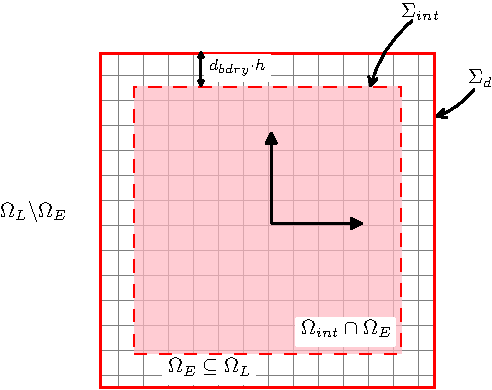
\includegraphics[width=0.5\linewidth]{./figures/hybrid/lambOseen/hlo_dd-crop.pdf}
	\caption{The domain decomposition for the Lamb-Oseen vortex problem, $\Omega_E \subseteq \Omega_L$. The Eulerian domain bounds $\Omega_E = [-1,1]\times[-1,1]$ with Dirichlet boundary $\partial \Omega_{dirichlet}$ [{\color{plotRed}{---}}, solid red] (\emph{not to scale}).}
	\label{fig:HLO_dc}
	\end{figure}

Figure \ref{fig:HLO_dc} shows the Hybrid domain configuration for the Lamb-Oseen Vortex problem with the Lagrangian domain $\Omega_L$ spanning the full fluid domain. The Eulerian domain $\Omega_E$ only resolves the center of the Lamb-Oseen core, $\Omega_E \subseteq \Omega_L$. The domain bounds $[-0.5,-0.5] \times [-0.5,-0.5]$ with a Dirichlet velocity boundary $\Sigma_d$ where the velocity boundary condition is applied as described in section 
\ref{subsec:dbc}. The correction of the Lagrangian domain is performed in the interpolation domain $\Omega_{int}$ according to the procedures described in section \ref{sec:correction}.

The spatial discretization of the Eulerian domain $\Omega_E$ is regarded as the control variable. Therefore, the parameter sensitivity analysis is performed by varying the spatial discretization of the Lagrangian method. The Eulerian domain is discretized with an unstructured mesh formulation using GMSH (see section \ref{subsec:mgugmsh}) having $N_{cells} = 226448$ unstructured cells and grid size $h_{grid}$ spanning $0.007$ to $0.0016$. 

The Lamb-Oseen Vortex problem is defined according to the parameters tabulated in table \ref{tab:HLO_pt}. The core is located at $(0,0)$, where the Eulerian domain $\Omega_E$ is centered. The parameters are chosen such that vorticity $\omega$ and velocity $\mathbf{u}$ is non-zero at the boundary of the Eulerian domain $\Sigma_d$, figure \ref{fig:HLO_dc}. 

The evolution of the Lagrangian solver and the Eulerian solver is performed according to section \ref{sec:evolveLagrangian} and \ref{sec:evolveEulerian} respectively. The Lagrangian solver performs TRS for diffusion of the vortex blobs, see section \ref{subsubsec:srs}. The scheme requires vortex blob redistribution at every step, $f_{redis} = 1$. In conjunction with the redistribution, the population control is performed at every step, $f_{pc}=1$ with $\Gamma_{thre}$ in table \ref{tab:HLO_pt}. 


\subsection{Results and Discussion}

The investigation of the Lamb-Oseen vortex problem is divided into three parts. The first part of the investigation concerns with comparing several stages of the hybrid coupling, section \ref{subsec:UvOvF}, where we compare the uncoupled scheme with the one-way coupled scheme and fully coupled scheme. These successive coupling investigate will help determine the source and quantify the error of the coupling. The second part of the investigation, section \ref{subsubsec:coc} focuses on importance of conservation of circulation that was discussed in section \ref{subsubsec:cc}. The results of the non-conserved and conserved scheme are compared to conclude the importance of conservation of circulation. During these two investigations, the parameters tabulated in table \ref{tab:HLO_pt} are used.

The third and final investigation is dedicated to the parameter sensitivity analysis, section \ref{subsubsec:psa}. Parameters that determine the spatial and temporal discretization of the scheme is investigated to verify the convergence of scheme.

\subsection{Uncoupled vs. One-way Coupled vs. Fully Coupled}
\label{subsec:UvOvF}
To verify the implementation of the hybrid algorithm, we compared several stages of the hybrid coupling with the standard, fully Eulerian test case. The three types of the coupling are as given:

\begin{itemize}
\item \textbf{Uncoupled}: The uncoupled test case involves only Eulerian solver and serves as a benchmark to quantify the error in coupling. The boundary conditions are determined directly from the analytical formulation, equation 	\ref{eq:eLO_veq}.
\item \textbf{One-way coupled}: The one-way coupled test case is a partially coupled hybrid test case where the Eulerian method is evolved using the Lagrangian solution. The correction of the Lagrangian solution is not performed in this scenario. Thus, this case will help us determine the error in evolution Eulerian method using the Lagrangian solution.
\item \textbf{Fully coupled}: The fully coupled test case performs the full coupling strategy described in section \ref{subsec:mcs}. The Eulerian method is evolved using the Lagrangian solution and the Lagrangian solution in the interpolation domain $\Omega_{int}$, figure \ref{fig:HLO_dc} is corrected at the end of each time step. This test case will help us quantify the error in transferring the Eulerian solution to the Lagrangian method.
\end{itemize}
	
	\begin{figure}[h]
     \centering
     \begin{subfigure}[t]{0.45\textwidth}
             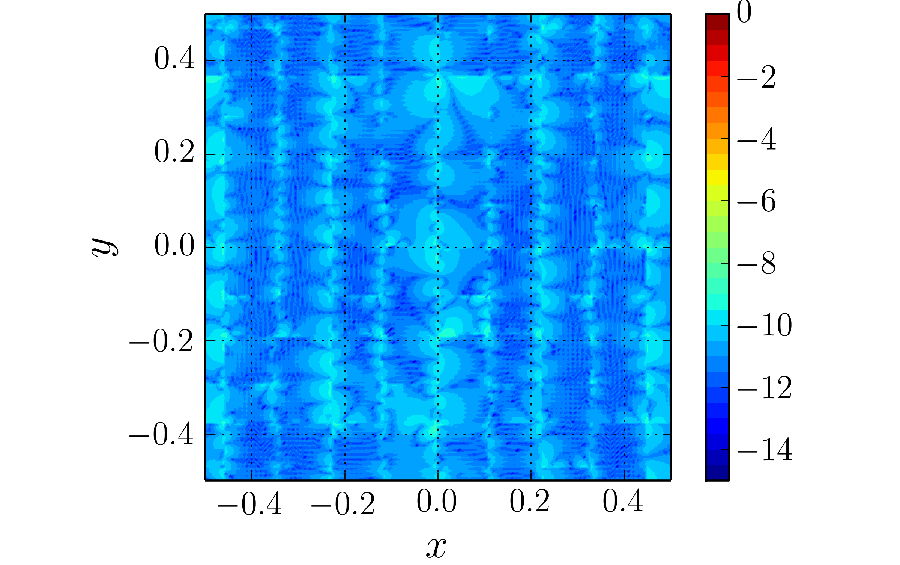
\includegraphics[width=\linewidth]{./figures/hybrid/lambOseen/lambOseen_fully_vErrorInitial_raster.pdf}
             \caption{Velocity}
             \label{fig:lambOseen_oneway_vErrorInitial}
     \end{subfigure}%
     \qquad %add desired spacing between images, e. g. ~, \quad, \qquad etc.
       %(or a blank line to force the subfigure onto a new line)
     \begin{subfigure}[t]{0.45\textwidth}
             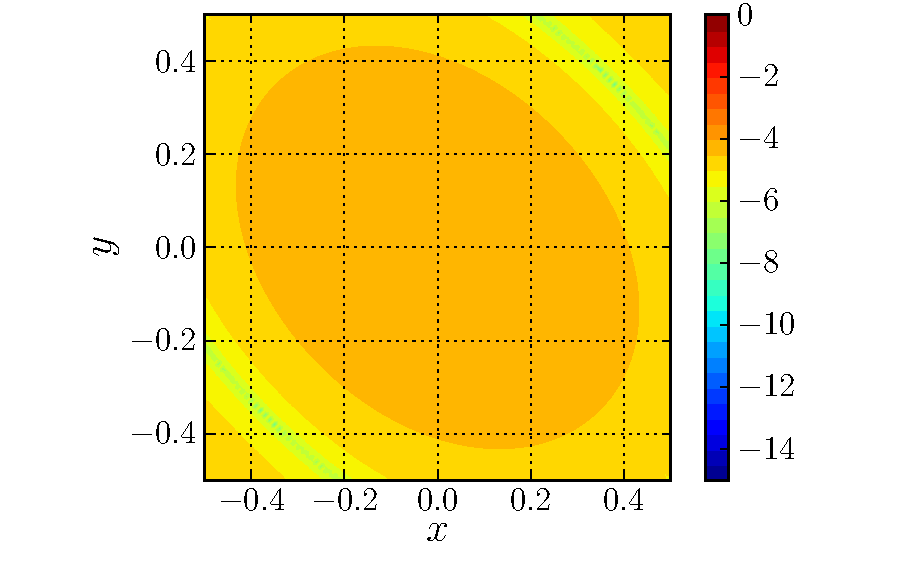
\includegraphics[width=\linewidth]{./figures/hybrid/lambOseen/lambOseen_fully_wErrorInitial_compressed.pdf}
             \caption{Vorticity}
             \label{fig:lambOseen_uncoupled_wErrorInitial}
     \end{subfigure}
     \caption{Initial relative error at $t=0$ inside the Eulerian domain. The figure depicts \textbf{(a)} the relative error in velocity $\mathbf{u}$ and \textbf{(b)} the relative error in vorticity $\omega$.}
     \label{fig:lambOseen_initialError}
	\end{figure}
		
Figure \ref{fig:lambOseen_initialError} depicts the initial relative error in velocity and vorticity inside the Eulerian domain $\Omega_E$. The relative error in velocity is near machine epsilon $\epsilon \le \num{10e-8}$, but the error in vorticity is in the order \num{10e-5}. Similar observation was made in section \ref{subsec:eulerianLambOseen} and arises from the projection error when determining the vorticity from velocity. The error is dependent on the type of discretization and we have second-order velocity space and first-order vorticity space. 

	\begin{figure}[!t]
	\centering
	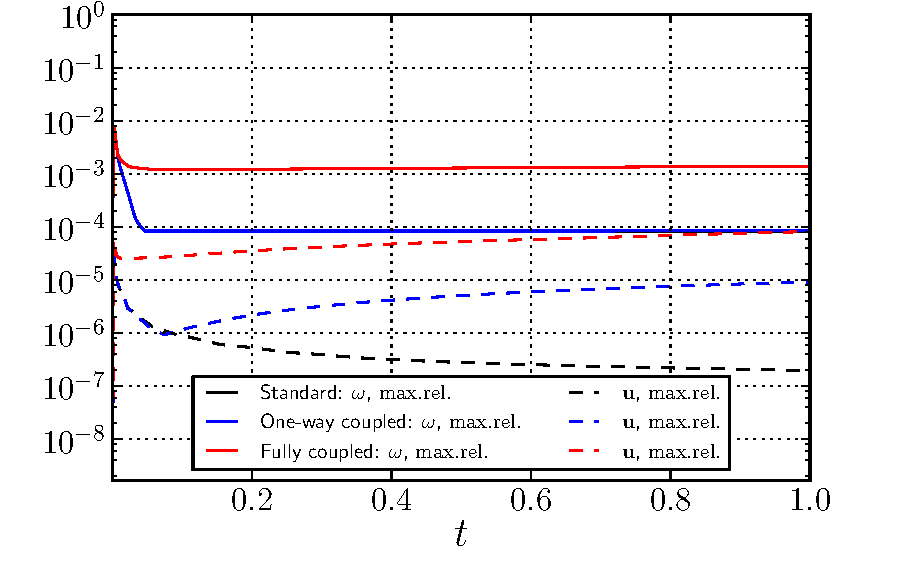
\includegraphics[width=0.6\linewidth]{./figures/hybrid/lambOseen/lambOseen_comparision_compressed.pdf}
	\caption{Comparison of the evolution of the maximum relative error from $t=0$ to $t=1$. The figure compares standard case (\textbf{black}) vs. the one-way coupled case ({\color{plotBlue}{\textbf{blue}}}) vs. the fully coupled case ({\color{plotRed}{\textbf{red}}}). The plot depicts maximum relative error in velocity (dashed), and the maximum relative error in vorticity (solid).}
	\label{fig:lambOseen_comparison}
	\end{figure}

The simulation is evolved from $t=0$ to $t=1$ with $N_{t-steps} = 1000$ Lagrangian and Eulerian time steps using the time step parameters tabulated in table \ref{tab:HLO_pt}. Figure \ref{fig:lambOseen_comparison} shows the evolution of maximum relative error in vorticity $\omega$ and velocity $\mathbf{u}$ of the uncoupled, one-way coupled and the fully coupled cases in the Eulerian domain $\Omega_E$ w.r.t. the analytical solution, equation \ref{eq:lo_voeq}. The initial observation shows the error in velocity is two to three orders of magnitude less than the error in vorticity and occurs due to the projection error. The figure shows that the uncoupled scheme has the lowest error in vorticity and velocity. As the boundary condition is directly obtained from the analytical solution, the error only arises from FE discretization of the Eulerian method. As time progresses, the error in velocity converges around \num{10e-7} and the error in vorticity converges around \num{10e-4}.

The one-way coupled case shows an increase in the velocity field inside the Eulerian domain $\Omega_E$. The increase in error is negligible at the initial stages of the coupling. This states that the discretization error of the analytical solution is well represented using the vortex blobs. At $t=1$, the error in velocity increases by two orders of magnitude from \num{10e-7} to \num{10e-5}. This implies that the error is due to the growth in error of the Lagrangian field. In chapter \ref{ch:lagrangian}, we observed there is an increase in the error due to the circulation processing techniques (population control, remeshing) and the time-marching of the vortex blobs.

The fully coupled case demonstrates that there is further increase in the error in velocity. Moreover, we observe that the there is now an increase in error in vorticity as well. As we are transfer the discrete vorticity field from the Eulerian method to the Lagrangian method it causes an increase in error of the Lagrangian solution. The consequence of this is that now the velocity field resolved by the Lagrangian method has an addition error. The figure depicts this effect, showing an increase in error in velocity. After the first few iteration (around $t=0.2$), there is a measurable difference between the fully coupled and the one-way coupled case. 

	
	\begin{figure}[h]
     \centering
     \begin{subfigure}[t]{0.45\textwidth}
             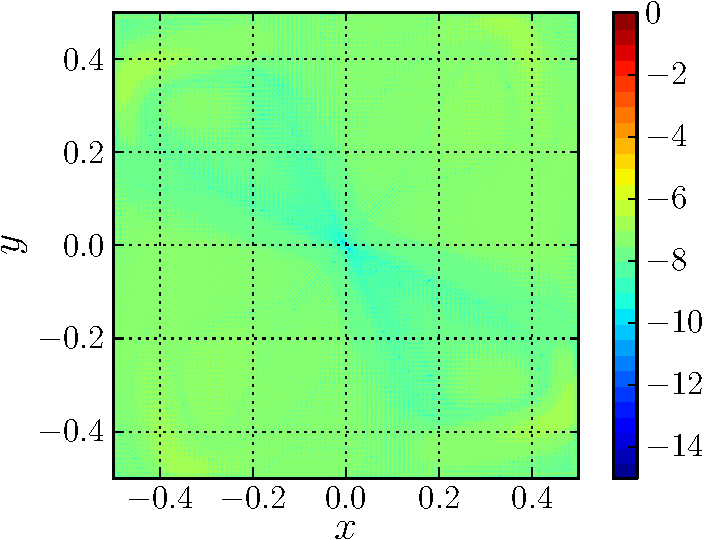
\includegraphics[width=\linewidth]{./figures/hybrid/lambOseent2/lambOseen_uncoupled_vErrorFinal_compressed-crop.pdf}
             \caption{Standard; velocity $\mathbf{u}$}
             \label{fig:lambOseen_uncoupled_vErrorFinal}
     \end{subfigure}%
     \qquad %add desired spacing between images, e. g. ~, \quad, \qquad etc.
       %(or a blank line to force the subfigure onto a new line)
     \begin{subfigure}[t]{0.45\textwidth}
             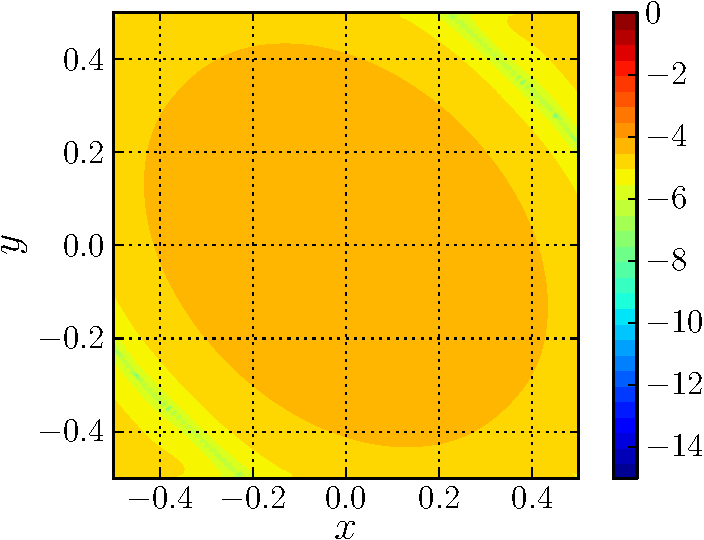
\includegraphics[width=\linewidth]{./figures/hybrid/lambOseent2/lambOseen_uncoupled_wErrorFinal_compressed-crop.pdf}
             \caption{Standard; vorticity $\omega$}
             \label{fig:lambOseen_uncoupled_wErrorFinal}
     \end{subfigure}%       
       
     \begin{subfigure}[t]{0.45\textwidth}
             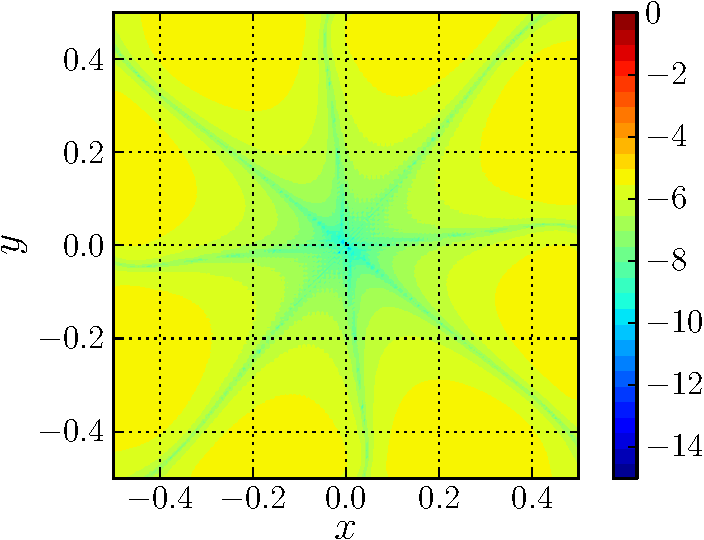
\includegraphics[width=\linewidth]{./figures/hybrid/lambOseent2/lambOseen_oneway_vErrorFinal_compressed-crop.pdf}
             \caption{One-way coupled; velocity $\mathbf{u}$}
             \label{fig:lambOseen_oneway_vErrorFinal}
     \end{subfigure}
     \qquad
     \begin{subfigure}[t]{0.45\textwidth}
             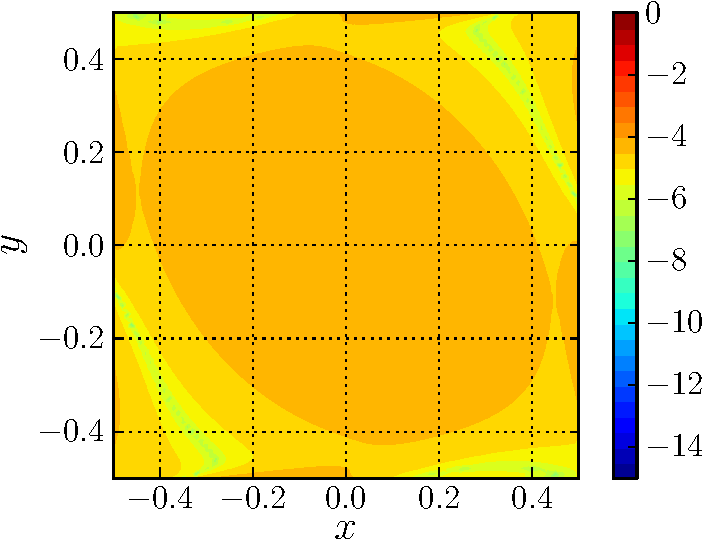
\includegraphics[width=\linewidth]{./figures/hybrid/lambOseent2/lambOseen_oneway_wErrorFinal_compressed-crop.pdf}
             \caption{One-way coupled; vorticity $\omega$}
             \label{fig:lambOseen_oneway_wErrorFinal}
     \end{subfigure}     
   
     \begin{subfigure}[t]{0.45\textwidth}
             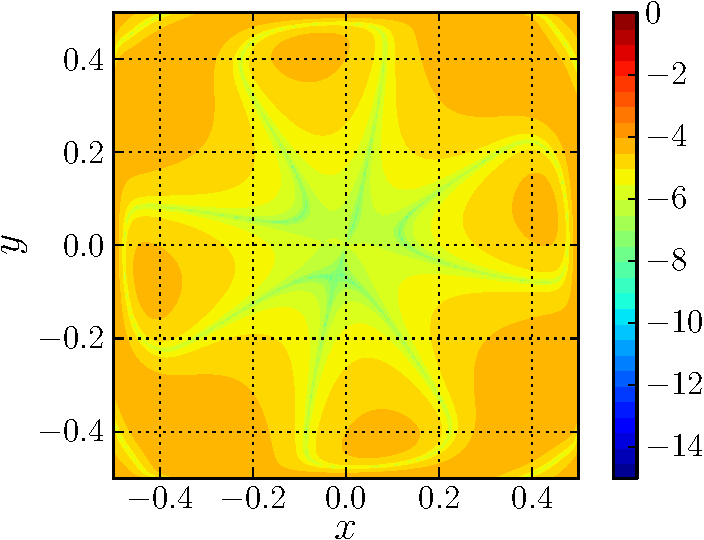
\includegraphics[width=\linewidth]{./figures/hybrid/lambOseent2/lambOseen_fully_vErrorFinal_compressed-crop.pdf}
             \caption{Fully coupled; velocity $\mathbf{u}$}
             \label{fig:lambOseen_fully_vErrorFinal}
     \end{subfigure}     
     \qquad
     \begin{subfigure}[t]{0.45\textwidth}
             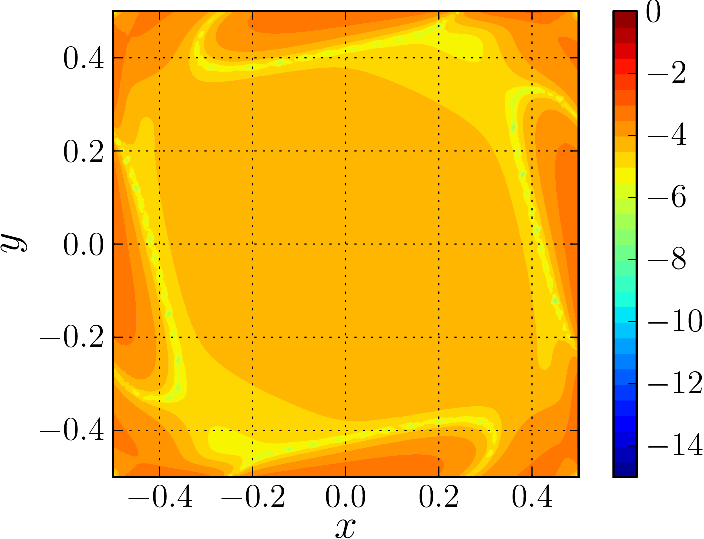
\includegraphics[width=\linewidth]{./figures/hybrid/lambOseent2/lambOseen_fully_wErrorFinal_compressed-crop.pdf}
             \caption{Fully coupled; vorticity $\omega$}
             \label{fig:lambOseen_fully_wErrorFinal}
     \end{subfigure}        
     
     \caption{Initial relative error at $t=0$ inside the Eulerian domain. The figure depicts \textbf{(a)} the relative error in velocity $\mathbf{u}$ and \textbf{(b)} the relative error in vorticity $\omega$.}
     \label{fig:lambOseen_finalError}
	\end{figure}	


\subsubsection*{Conservation of circulation}
\label{subsubsec:coc}

	\begin{figure}[h]
     \centering
     \begin{subfigure}[t]{0.45\textwidth}
             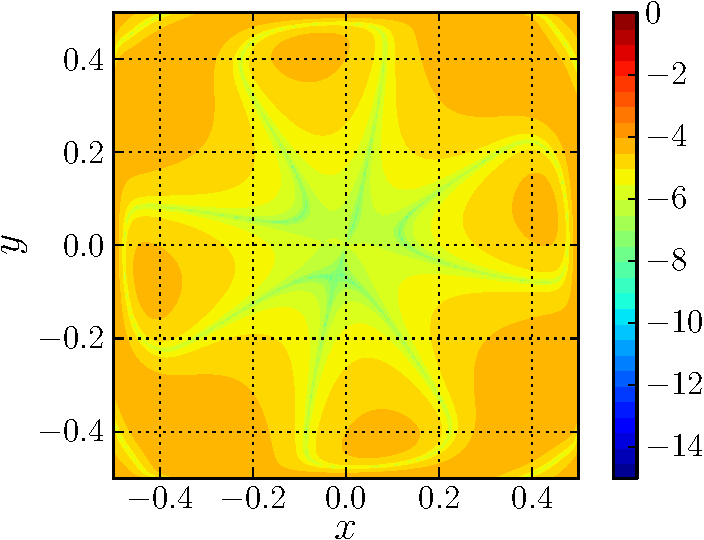
\includegraphics[width=\linewidth]{./figures/hybrid/lambOseent2/lambOseen_fully_vErrorFinal_compressed-crop.pdf}
             \caption{Conservation \texttt{on}; velocity $\mathbf{u}$}
             \label{fig:lambOseen_fullyCon_vErrorFinal}
     \end{subfigure}%
     \qquad %add desired spacing between images, e. g. ~, \quad, \qquad etc.
       %(or a blank line to force the subfigure onto a new line)
     \begin{subfigure}[t]{0.45\textwidth}
             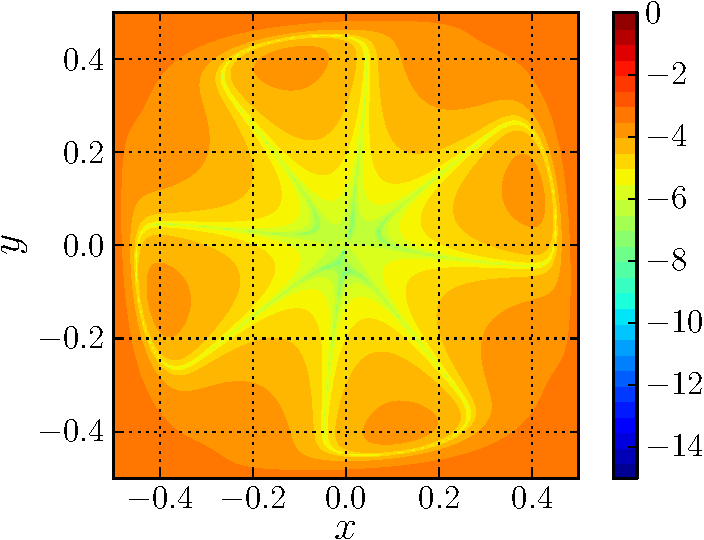
\includegraphics[width=\linewidth]{./figures/hybrid/lambOseent2/lambOseen_fullyCoff_vErrorFinal_compressed-crop.pdf}
             \caption{Conservation \texttt{off}; velocity $\mathbf{u}$}
             \label{fig:lambOseen_fullyCoff_vErrorFinal}
     \end{subfigure}
     
    \begin{subfigure}[t]{0.45\textwidth}
             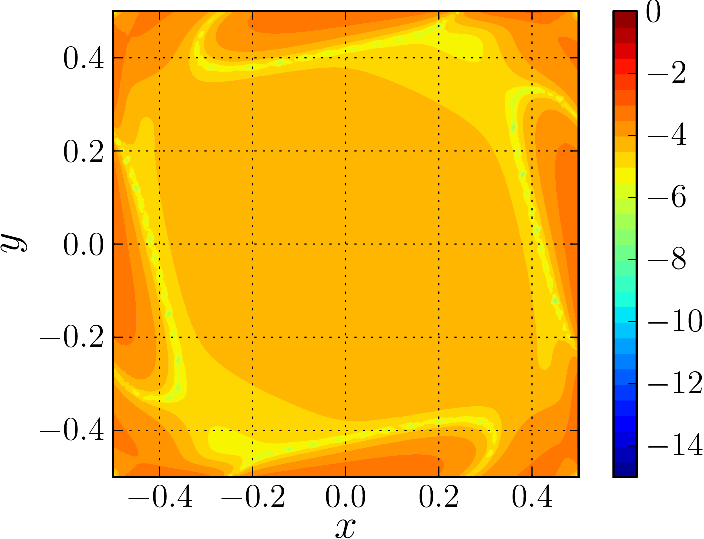
\includegraphics[width=\linewidth]{./figures/hybrid/lambOseent2/lambOseen_fully_wErrorFinal_compressed-crop.pdf}
             \caption{Conservation \texttt{on}; vorticity $\omega$}
             \label{fig:lambOseen_fullyCon_wErrorFinal}
     \end{subfigure}%         
     \qquad     
     \begin{subfigure}[t]{0.45\textwidth}
             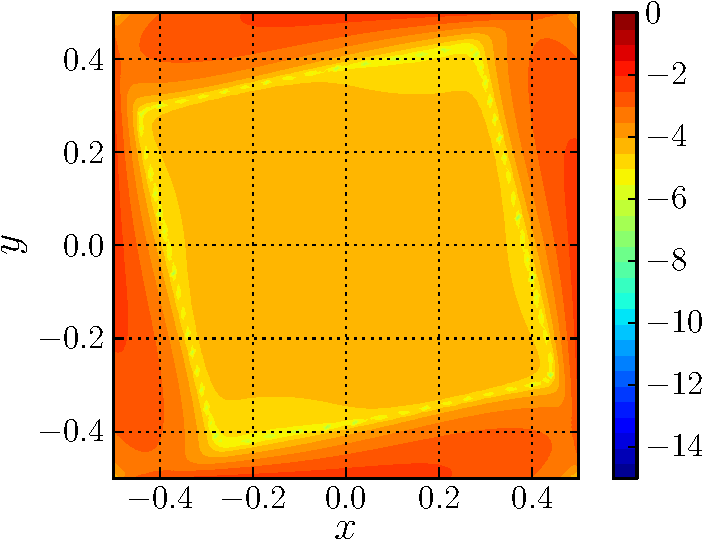
\includegraphics[width=\linewidth]{./figures/hybrid/lambOseent2/lambOseen_fullyCoff_wErrorFinal_compressed-crop.pdf}
             \caption{Conservation \texttt{off}; vorticity $\omega$}
             \label{fig:lambOseen_fullyCoff_wErrorFinal}
     \end{subfigure}  

           
  
     \caption{Initial relative error at $t=0$ inside the Eulerian domain. The figure depicts \textbf{(a)} the relative error in velocity $\mathbf{u}$ and \textbf{(b)} the relative error in vorticity $\omega$.}
     \label{fig:lambOseen_conservation_contourf}
	\end{figure}


	\begin{figure}[h]
     \centering
     \begin{subfigure}[t]{0.45\textwidth}
             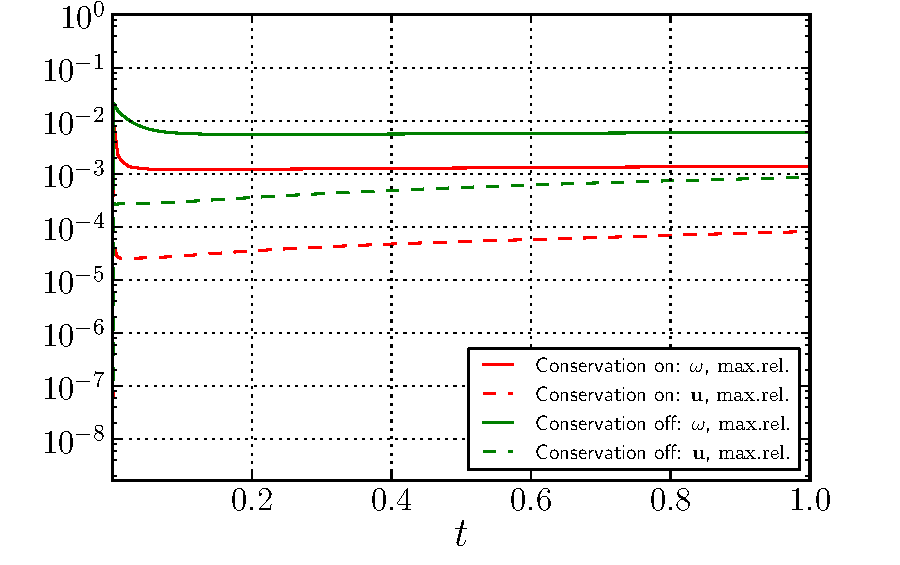
\includegraphics[width=\linewidth]{./figures/hybrid/lambOseent2/lambOseen_comparision_conservation_compressed.pdf}
             \caption{Relative Error in velocity and vorticity}
             \label{fig:lambOseen_comparision_conservation}
     \end{subfigure}%
     \qquad %add desired spacing between images, e. g. ~, \quad, \qquad etc.
       %(or a blank line to force the subfigure onto a new line)
     \begin{subfigure}[t]{0.45\textwidth}
             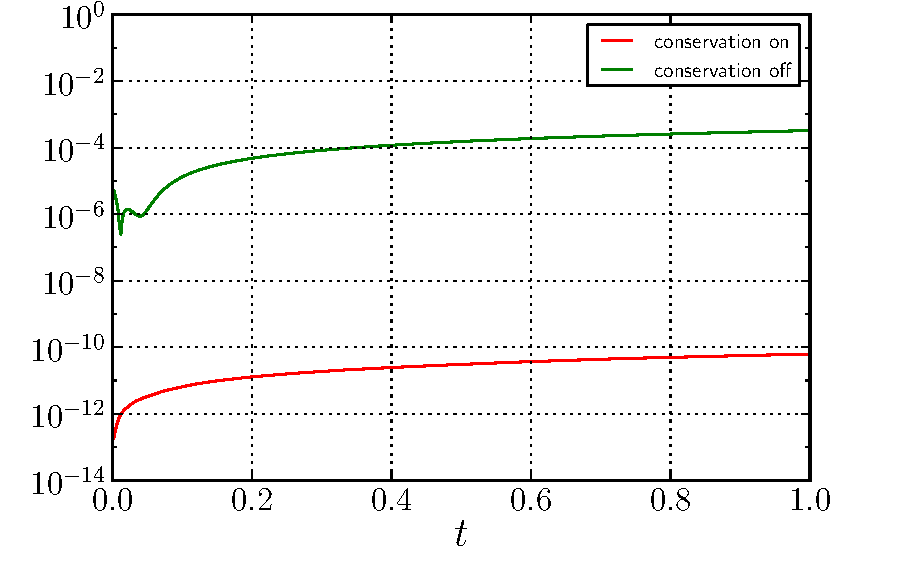
\includegraphics[width=\linewidth]{./figures/hybrid/lambOseent2/lambOseen_comparision_conservation_circulation_compressed.pdf}
             \caption{Error in total circulation $\Gamma$}
             \label{fig:lambOseen_comparision_conservation_circulation}
     \end{subfigure}%       
     \caption{Initial relative error at $t=0$ inside the Eulerian domain. The figure depicts \textbf{(a)} the relative error in velocity $\mathbf{u}$ and \textbf{(b)} the relative error in vorticity $\omega$.}
     \label{fig:lambOseen_conservation_comparisions}
	\end{figure}


\subsubsection{Parameter sensitiviy analysis}
\label{subsubsec:psa}

\subsection{Conclusion}



\section{Clercx-Bruneau Dipole Collision}

\subsection{Problem Definition}

\subsection{Results}

\subsection{Conclusion}

%
%\section{Clercx-Bruneau Dipole Collision}
%
%\subsection{Problem Definition}
%
%\subsection{Results}
%
%\subsection{Conclusion}

%
%	\begin{figure}[h]
%     \centering
%     \begin{subfigure}[t]{0.45\textwidth}
%             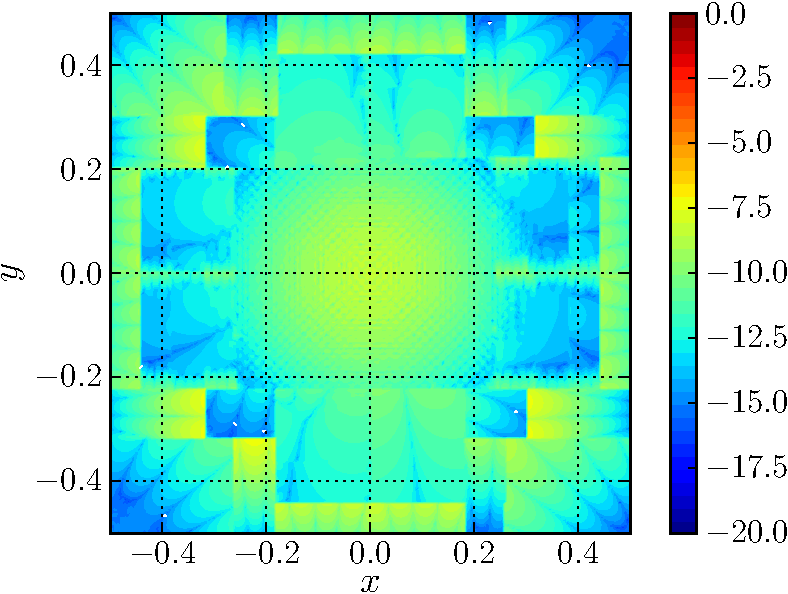
\includegraphics[width=\linewidth]{./figures/hybrid/lambOseen_standard_vErrorInitial_compressed-crop.pdf}
%             \caption{Velocity}
%             \label{fig:lambOseen_standard_vErrorInitial}
%     \end{subfigure}%
%     \qquad %add desired spacing between images, e. g. ~, \quad, \qquad etc.
%       %(or a blank line to force the subfigure onto a new line)
%     \begin{subfigure}[t]{0.45\textwidth}
%             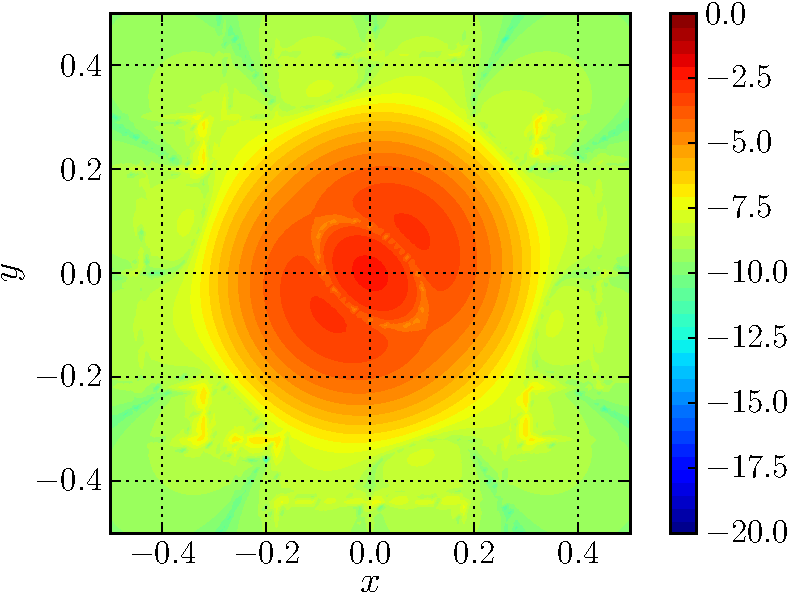
\includegraphics[width=\linewidth]{./figures/hybrid/lambOseen_standard_wErrorInitial_compressed-crop.pdf}
%             \caption{Final Error}
%             \label{fig:lambOseen_standard_wErrorInitial}
%     \end{subfigure}
%     \caption{Initial Error of the Lamb-Oseen vortex}
%     \label{fig:lambOseen_initialError}
%	\end{figure}
%	
	

%	\begin{figure}[h]
%     \centering
%     \begin{subfigure}[t]{0.45\textwidth}
%             \includegraphics[width=\linewidth]{./figures/hybrid/lambOseen_vErrorInitial_compressed-crop.pdf}
%             \caption{Initial Error}
%             \label{fig:lambOseen_vErrorInitial_compressed-crop}
%     \end{subfigure}%
%     ~ %add desired spacing between images, e. g. ~, \quad, \qquad etc.
%       %(or a blank line to force the subfigure onto a new line)
%     \begin{subfigure}[t]{0.45\textwidth}
%             \includegraphics[width=\linewidth]{./figures/hybrid/lambOseen_vErrorFinal_k1_compressed-crop.pdf}
%             \caption{Final Error}
%             \label{fig:lambOseen_vErrorFinal_k1_compressed}
%     \end{subfigure}
%     \caption{Growth in error, velocity max. relative error, dtl=dte, h=0.02, dte=0.001}
%     \label{fig:lambOseen_vError}
%	\end{figure}
%	
%	\begin{figure}[h]
%     \centering
%     \begin{subfigure}[t]{0.45\textwidth}
%             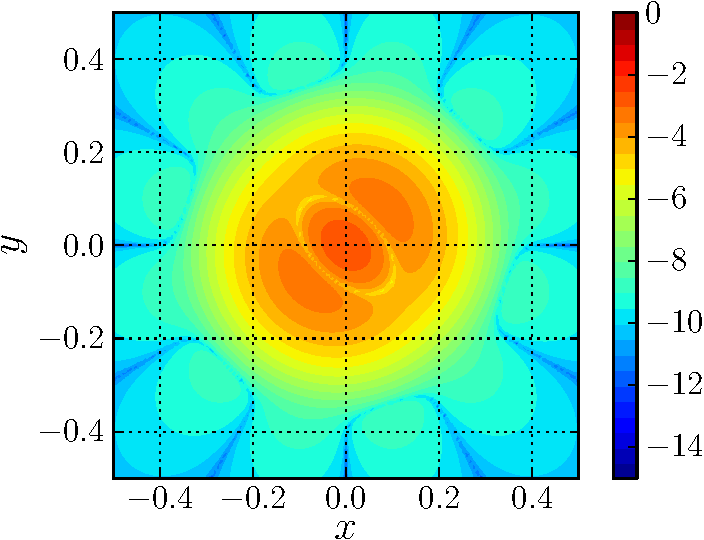
\includegraphics[width=\linewidth]{./figures/hybrid/lambOseen_wErrorInitial_compressed-crop.pdf}
%             \caption{Initial Error}
%             \label{fig:lambOseen_wErrorInitial_compressed}
%     \end{subfigure}%
%     ~ %add desired spacing between images, e. g. ~, \quad, \qquad etc.
%       %(or a blank line to force the subfigure onto a new line)
%     \begin{subfigure}[t]{0.45\textwidth}
%             \includegraphics[width=\linewidth]{./figures/hybrid/lambOseen_wErrorFinal_k1_compressed-crop.pdf}
%             \caption{Final Error}
%             \label{fig:lambOseen_wErrorFinal_k1_compressed}
%     \end{subfigure}
%     \caption{Growth in error, vorticity max. relative error, dtl=dte, h=0.02, dte=0.001}
%     \label{fig:lambOseen_wError}
%	\end{figure}	
	
\subsection{Variation in Lagrangian time step size}	
	
%	\begin{figure}[h]
%		\centering
%		\begin{subfigure}[t]{0.45\textwidth}
%		      \includegraphics[width=\linewidth]{./figures/hybrid/lambOseen_vErrorFinal_k1_compressed-crop.pdf}
%		      \caption{$k=1$}
%		      \label{fig:lambOseen_vErrorFinal_k1}
%		\end{subfigure}%
%		~ %add desired spacing between images, e. g. ~, \quad, \qquad etc.
%		%(or a blank line to force the subfigure onto a new line)
%		\begin{subfigure}[t]{0.45\textwidth}
%		      \includegraphics[width=\linewidth]{./figures/hybrid/lambOseen_vErrorFinal_k2_compressed-crop.pdf}
%		      \caption{$k=2$}
%		      \label{fig:lambOseen_vErrorFinal_k2}
%		\end{subfigure}
%		~
%		\begin{subfigure}[t]{0.45\textwidth}
%		      \includegraphics[width=\linewidth]{./figures/hybrid/lambOseen_vErrorFinal_k5_compressed-crop.pdf}
%		      \caption{$k=5$}
%		      \label{fig:lambOseen_vErrorFinal_k5}
%		\end{subfigure}		
%		~
%		\begin{subfigure}[t]{0.45\textwidth}
%		      \includegraphics[width=\linewidth]{./figures/hybrid/lambOseen_vErrorFinal_k10_compressed-crop.pdf}
%		      \caption{$k=5$}
%		      \label{fig:lambOseen_vErrorFinal_k10}
%		\end{subfigure}			
%		
%		\caption{Variation in the Lagrangian k, velocity max. relative error, dtl=k*dte, h=0.02, dte=0.001}
%		\label{fig:lambOseen_vError_k}
%	\end{figure}
%	
%	
%	\begin{figure}[h]
%		\centering
%		\begin{subfigure}[t]{0.45\textwidth}
%		      \includegraphics[width=\linewidth]{./figures/hybrid/lambOseen_wErrorFinal_k1_compressed-crop.pdf}
%		      \caption{$k=1$}
%		      \label{fig:lambOseen_wErrorFinal_k1}
%		\end{subfigure}%
%		~ %add desired spacing between images, e. g. ~, \quad, \qquad etc.
%		%(or a blank line to force the subfigure onto a new line)
%		\begin{subfigure}[t]{0.45\textwidth}
%		      \includegraphics[width=\linewidth]{./figures/hybrid/lambOseen_wErrorFinal_k2_compressed-crop.pdf}
%		      \caption{$k=2$}
%		      \label{fig:lambOseen_wErrorFinal_k2}
%		\end{subfigure}
%		~
%		\begin{subfigure}[t]{0.45\textwidth}
%		      \includegraphics[width=\linewidth]{./figures/hybrid/lambOseen_wErrorFinal_k5_compressed-crop.pdf}
%		      \caption{$k=5$}
%		      \label{fig:lambOseen_wErrorFinal_k5}
%		\end{subfigure}		
%		~
%		\begin{subfigure}[t]{0.45\textwidth}
%		      \includegraphics[width=\linewidth]{./figures/hybrid/lambOseen_wErrorFinal_k10_compressed-crop.pdf}
%		      \caption{$k=5$}
%		      \label{fig:lambOseen_wErrorFinal_k10}
%		\end{subfigure}			
%		
%		\caption{Variation in the Lagrangian k, velocity max. relative error, dtl=k*dte, h=0.02, dte=0.001}
%		\label{fig:lambOseen_wError_k}
%	\end{figure}		
	
	
%	\begin{figure}[h]
%	\centering
%	\includegraphics[width=0.5\linewidth]{./figures/hybrid/daeninck_CylinderVorticity.png}
%	\caption{Result of hybrid coupling by Daeninck \cite{Daeninck2006}. The figure shows artificial vorticity at the boundary of the Eulerian domain.}
%	\label{fig:daeninck_CylinderVorticity}
%	\end{figure}




\section{Error in coupling: Verification with Lamb-Oseen vortex}

	\subsection{Generation of artificial vorticity}


\section{Clercx-Bruneau dipole convection at $Re=625$}

	\subsection{Comparison of vorticity contours}
	
	\subsection{Variation in maximum vorticity}
	
	\subsection{Variation in kinetic energy}
	
	\subsection{Variation in enstrophy}

\section{Clercx-Bruneau dipole collision at $Re=625$}

	\subsection{Comparison of vorticity contours}
	
	\subsection{Variation in maximum vorticity}
	
	\subsection{Variation in kinetic energy}
	
	\subsection{Variation in Enstrophy}
	
	\subsection{Variation in Palinstrophy}

\section{Impulsively started cylinder problem at $Re=550$}

	\subsection{Evolution of the wake}
	
	\subsection{Evolution of pressure and friction drag}
	
	\subsection{Evolution of lift}

\section{Moving body}

	\subsection{Error due to pertubation lag}

\section{Proof of concepts}

	\subsection{Multiple cylinder case}
	
	\subsection{Stalled airfoil at $Re=5000$}

\section{Summary}
	%
	% Chapter 6: Applications of Hybrid vortex method
	%\chapter{Application of the Hybrid Vortex Method}
%\label{ch:LiteratureReview}

% Comparison of hybrid vortex methods.
% choice of hybrid method. Example domain decomposion, coupling technique

\section{Application of Hybrid Vortex method for a 2D VAWT}

\subsection{Reference setup}

\subsection{Instantaneous flow-field}

\subsection{Time averaged flow-field}

\subsection{Near-wake}

\subsubsection{Dynamic Stall of the airfoil}

\subsection{Far-wake}

\subsubsection{Blade-wake interaction}

\section{Feasibility of Hybrid Vortex method for compressor cascade}

\subsection{Assumptions and approximations}

\subsection{Advantages of hybrid vortex method}

\subsection{Limitation of using hybrid vortex method}

\subsection{Proposed solution}



%\section{Former Work}
%\label{sec:FormerWork}
%
%\subsection{Overview of the Work}
%\label{subsec:OverviewoftheWork}

%\section{Purpose of further research}

%%%%%%%%%%%%%%%%%%%%%%%%%%%%%%%%%%%%%%%%%%%%%%%%%%%%%%%%%%%%%%%%%%%%
%\nomenclature[ak]{$K$}{Kelvin (temperature)}
%\nomenclature[ar]{rpm}{Revolutions per minute (frequency)}
%\nomenclature[ac]{CO}{Carbon Monoxide}
%\nomenclature[ac]{CRM}{Chemical Reaction Modelling}
%\nomenclature[ah]{H2}{Molecular hydrogen}
%\nomenclature[ag]{GSP}{Gas Turbine Simulation Program (Software)}
%\nomenclature[rr]{$\rho$}{Density \nomunit{[$kg/{m^3}$]}}
%\nomenclature[sm]{$\dot{m}$}{Mass flow rate \nomunit{[$kg/s$]}}
%\nomenclature[ab]{bar}{Pressure}

%\nomenclature[rr]{$Re$}{Reynolds number \nomunit{[-]}}
%\nomenclature[rw]{$M$}{Mach number \nomunit{[-]}}
%\nomenclature[rw]{$\mu$}{Dynamic viscosity of air \nomunit{[$kg/{s \cdot m}$]}}
    
    % Chapter 7: 
	\chapter{Conclusion and Recommendation}
\label{ch:ConclusionandRecommendation}

\section{Conclusion}

\subsection{Feasibility of hybrid vortex method for compressor cascade}

\section{Recommendations}

\subsection{RBF kernel representation of boundary}

\subsection{Recommended numerical simulation for compressor cascade}
    
    %
    % Bibliography
    \printbib{/home/lento/Documents/Bibliography/library.bib}%
    %
    \appendix%
    %
    % and some appendices here
    \chapter{Mathematical Model}\label{app:math_model_main_rotor}%
    %
    \section{Introduction}%
        %
        This appendix contains the math model of the thesis. It looks as follows:
        %
        \begin{equation}
            c = \sqrt{a^2+b^2}
        \end{equation}
        %
        
        
        
        
        
        
%
    %
    %
\backmatter%
    %
    % index file here (not needed for a MSc thesis)
    %
\end{document}
